\chapter{Analysis strategy}
\label{ch:an_strategy}
\epigraph{\itshape``All men can see these tactics whereby I conquer, but what none can see is the strategy out of which victory is evolved."}{--- \textup{Sun Tzu}}

\section{Introduction}
\hspace{10pt}This chapter serves to present a detailed documentation of the analysis strategy used for the search for the invisibly decaying Higgs bosons, where the Higgs boson is produced via the Vector Boson Fusion production mechanism. The study at hand has had a long history within the CMS experiment starting all the way back from the early days of Run 1~\cite{paper:HIG_17_023}. This thesis tends to build on conclusions and methods achieved with previous efforts by improving them where possible, while also taking the advantage of the full Run 2 dataset.

\hspace{10pt} Each of the following sections is going to summarize motivations and definitions that came into fruition while forming two main categories. Special attention will be given to the analysis category based around new, production mode targeting triggers introduced in Section~\ref{sec:vbf_trgger}, which allowed for further exploration of the signal sensitive phase space. Being a large part of motivation influencing the selection requirements, performance studies of analysis related trigger algorithms are going to be presented at this stage. Finally, this chapter concludes with a discussion regarding additional data quality issues plaguing 2017 and 2018 eras of data taking and studies performed in order to mitigate their effects on the final result.

\hspace{10pt} In order to be consistent with the notation used in Chapter~\ref{ch:combination}, which combines results from all hadronic production modes of the Higgs boson, a simple naming convention is going to be used when addressing certain analyses (due to common motivations and data quality issues plaguing them). This convention is based on the two main focuses in terms of the preferred Higgs boson production mode. All studies focusing on the Higgs boson produced via the vector boson fusion will be grouped under one roof named the ``VBF analysis'', while the remaining modes of interest such as the ttH, gluon-gluon fusion (ggH) and the VH production will represent the ``non-VBF analysis''.
\section{Selection requirements}
\hspace{10pt} This section serves as summary of two main analysis categories. In order to simplify the way of addressing different categories within the VBF analysis, the following notation is going to be used in future text. All studies being built around the $E_{T,miss}$ and $H_{T,miss}$ triggers shown in Table~\ref{tab:metmht} are going to be part of the Missing Energy Trigger (MTR) category. On the other hand, the new category being formed through the usage of VBF production mode targeting triggers (listed in Table~\ref{tab:hlt_rates}) is going to be named the VBF Trigger (VTR) category. A complete set of information regarding the L1 seeds used as inputs to the HLT algorithms forming these analysis categories is given in the form of Table~\ref{a_tab:triggers}.

\hspace{10pt} The common ground for both categories is the approach to rejecting the contributions from major sources of SM background when forming the signal region (SR) through the implementation of object vetos. In order to battle the reducible contribution coming from main V+jets backgrounds a $\mu/e/\tau$ vetos are imposed. A similar approach is taken in order to contain the $\gamma$+jets processes with the a veto on photon objects being put in place. Finally, a b jet object veto requirement tends to remove the reducible background originating from top quark SM processes. The interpretation of the aforementioned vetos follows the strategy described in Section~\ref{sec:object_corr}, where it is stated that a veto weight is applied for simulation samples as opposed to a $N_{object}=0$ condition, which is being used for data. The following pages are going to introduce the main selection criteria for each of the categories.
\subsection{Missing Energy Trigger category}
\label{subsec:vbfselection}

\hspace{10pt} This category follows the strategy published with the results originating from data collected in 2016~\cite{paper:HIG_17_023}. It is represented with the requirements shown in Table~\ref{tab:selection_mtr}. With the set of object vetos already covered in the introduction, the discussion regarding the rest of the requirements can be split into two categories. Their origin can be traced to be either related to the topological properties expected from VBF jets, introduced in order to reduce a major contribution from SM processes, or they are purely motivated by the performance of HLT algorithms used for data collection.

\begin{table}[htbp]
\centering
%\small
\begin{tabular}{lcc}
    Variable                           & Selection                       & Target background \\
    \hline
    & & \\
    $\mu$ ($e$) veto               & $p_T > 10$~GeV,~$|\eta| < 2.4 (2.5)$  & $Z(ll)$~+jets,~$W(l\nu)$~+jets \\
    $\tau$ lepton veto                 & $p_T > 20$~GeV,~$|\eta| < 2.3$        & $Z(ll)$~+jets,~$W(l\nu)$~+jets  \\
    $\gamma$ veto                        & $p_T > 15$~GeV,~$|\eta| < 2.5$        & $\gamma$~+jets \\
    b jet veto                    &  $p_T > 20$~GeV,~$|\eta| < 2.4$  &  Top quark\\
        & & \\
    $E_{T,miss}$                          & ${>} 250$~GeV                          & QCD, top quark, $Z(ll)$~+jets \\
    $min\Delta\phi(j, E_{T,miss})$   &  $ {>} 0.5$ radians               & QCD \\
    $|$1$-E_{T,miss}^{Calo}/E_{T,miss}|$   &  $ {<} 0.5$               & QCD \\
        & & \\
    $p_{T,j_1}$ and $\eta_{j1}$   & ${>} 80$~GeV and $ |\eta| < 4.7$      & All \\
    $p_{T,j_2}$ and $\eta_{j2}$   & ${>} 40$~GeV and $ |\eta| < 4.7$      & All \\
    $\eta_{j1}\cdot\eta_{j2}$   & ${<}$ 0   & All \\

    $m_{jj}$                               & ${>} 200$~GeV  \\       
    $\Delta\eta_{jj}$                            & ${>} 1.0$  \\
    $\Delta\phi_{jj}$                            & ${<} 1.5$  \\
        & & \\
         \hline
\end{tabular}
\caption{Summary of the MTR selection requirements, accompanied with the target background processes affected by them~\cite{note:AN_19_257}}
\label{tab:selection_mtr}
\end{table}

\hspace{10pt} Starting with the topological information, the VBF signature is characterised with a jet pair which has a large geometrical separation and a large dijet mass. When interpreted in terms of the detector geometry (introduced in Section~\ref{sec:geometry}), this leads to conditions that jets, chosen as the two leading in $p_T$, have to be separated by a large value of $\Delta \eta$, a small $\Delta \phi$ and to have $\eta_{j1}\cdot\eta_{j2}<0$ by being in the opposite bisections of the experiment.

\hspace{10pt} Moving on from the purely topological properties, the next step is to try and determine which variables represent a good basis for additional lowering of the contribution coming from various sources of SM background. Variables such as the $min \Delta \phi (j, E_T^{miss})$\footnote{The minimal $\Delta\phi$ between the one of the four leading jets (ordered in $p_T$) and the $\vec{p}_{T, miss}$.} (where only the first four leading jets with $p_T > 30$~GeV enter the computation) allow for a better control of the QCD multijet background, Figure~\ref{fig:sr_n-1_shapes_1} shows its separation power using the N-1 selection\footnote{All of selection requirements are being applied but the one involving the variable of interest.} approach. With it showing combined background composition originating from simulation samples of SM processes being overlaid with the distribution of the signal, it can be seen that the requirement of $min \Delta \phi (j, E_{T,miss})>$~0.5 yields a significant reduction of QCD multijet backgrounds, without a large loss of signal sensitivity. Another useful requirement comes from the comparison of the offline (after the full reconstruction) and calorimeter only $E_{T,miss}$. A requirement that the relative difference is less than 50\% (when taking the offline $E_{T,miss}$ as reference) provides another way of rejecting events which contain energetic mismeasured jets originating from multijet processes. 

\hspace{10pt} As indicated at the beginning of this section, geometrical properties of the selected dijet object play a large role in the recognition of signal like events, as illustrated in Figure~\ref{fig:sr_n-1_shapes_1}. This comparison of $\Delta \eta_{jj}$ and $\Delta \phi_{jj}$ distributions between main backgrounds and signal shows a clear opening for a set of requirements which are going to further improve the selection. An optimisation procedure, taking into account the entire setup for the analysis (including the contributions from dedicated control regions), was performed~\cite{paper:HIG_17_023} in order to obtain thresholds presented in Table~\ref{tab:selection_mtr}. 

\hspace{10pt} Finally, there are requirements that are arising strictly from trigger limitations. This can be seen in the choice of the $E_{T,miss}$ threshold, where the requirement on it being larger than $250$~GeV was imposed in order to stay above the $95$~\% efficiency for the category-forming triggers, when measured in data. This efficiency gets above $99$~\% for the values of $E_{T,miss}>300$~GeV. A more detailed documentation of this measurement is given in Section~\ref{subsec:mtr_triggers}.

\hspace{10pt} Figure~\ref{fig:sr_n-1_shapes_2} shows data to simulation agreement for a selected set of main analysis variables after the application of the complete MTR selection for the 2017 era of data taking. Corresponding information regarding the SR for the 2018 era is given in Appendix~\ref{app:MTR_2018}. The scale of data to simulation disagreement illustrates the need for dedicated control regions in order to better estimate the irreducible part of the contribution originating from V+jets processes. The MTR category is constructed to represent the main analysis category, covering a large piece of the phase space of interest. In order to further improve on it, the following section is going to show a complementary category formed around a set of VBF triggers introduced in Section~\ref{sec:vbf_trgger}.

\begin{figure}[htbp]
  \centering
    \subfigure[$min\Delta\phi(j,E_T^{miss})$]{
    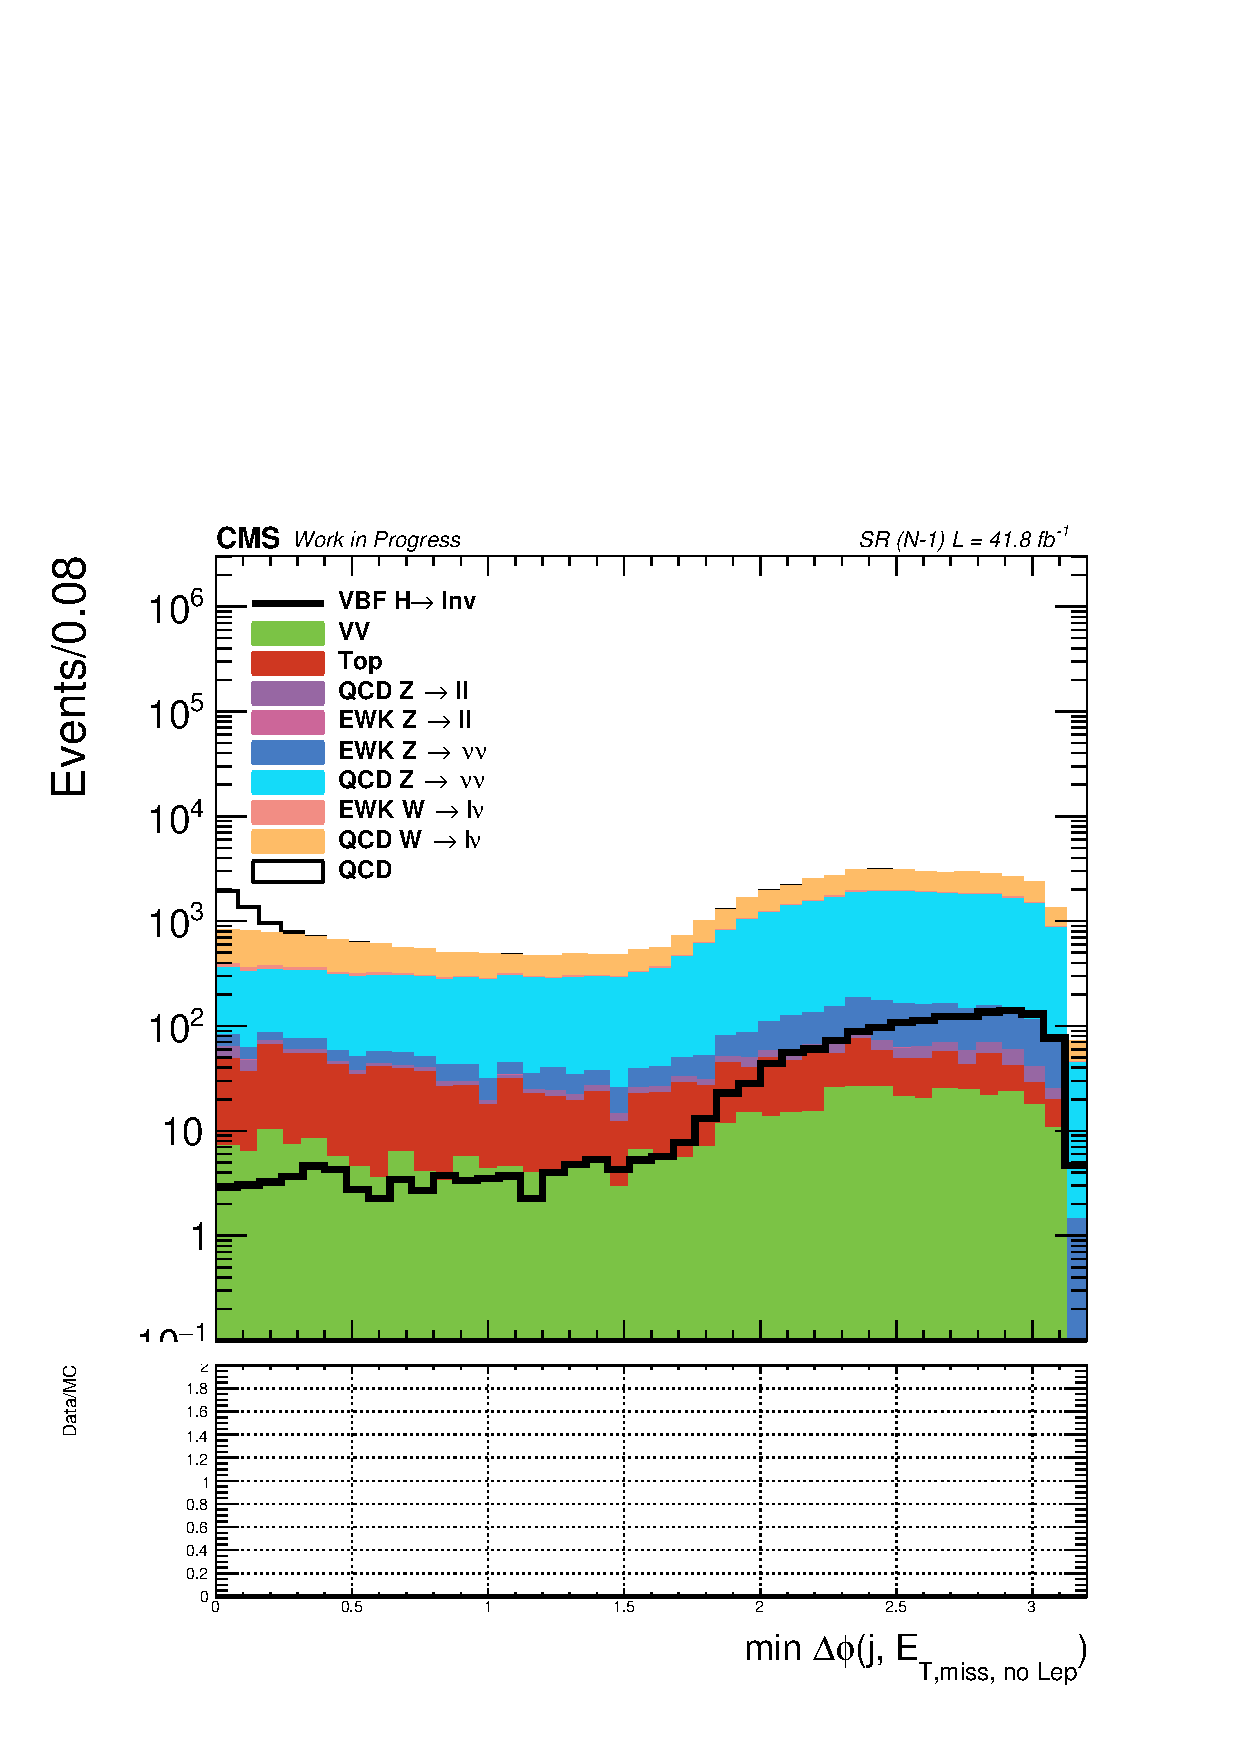
\includegraphics[width=0.49\textwidth]{Analysis_strategy/Nminus1/min_dphi_nminus1_log.pdf}
    }\\
    \subfigure[$\Delta \eta_{jj}$]{
    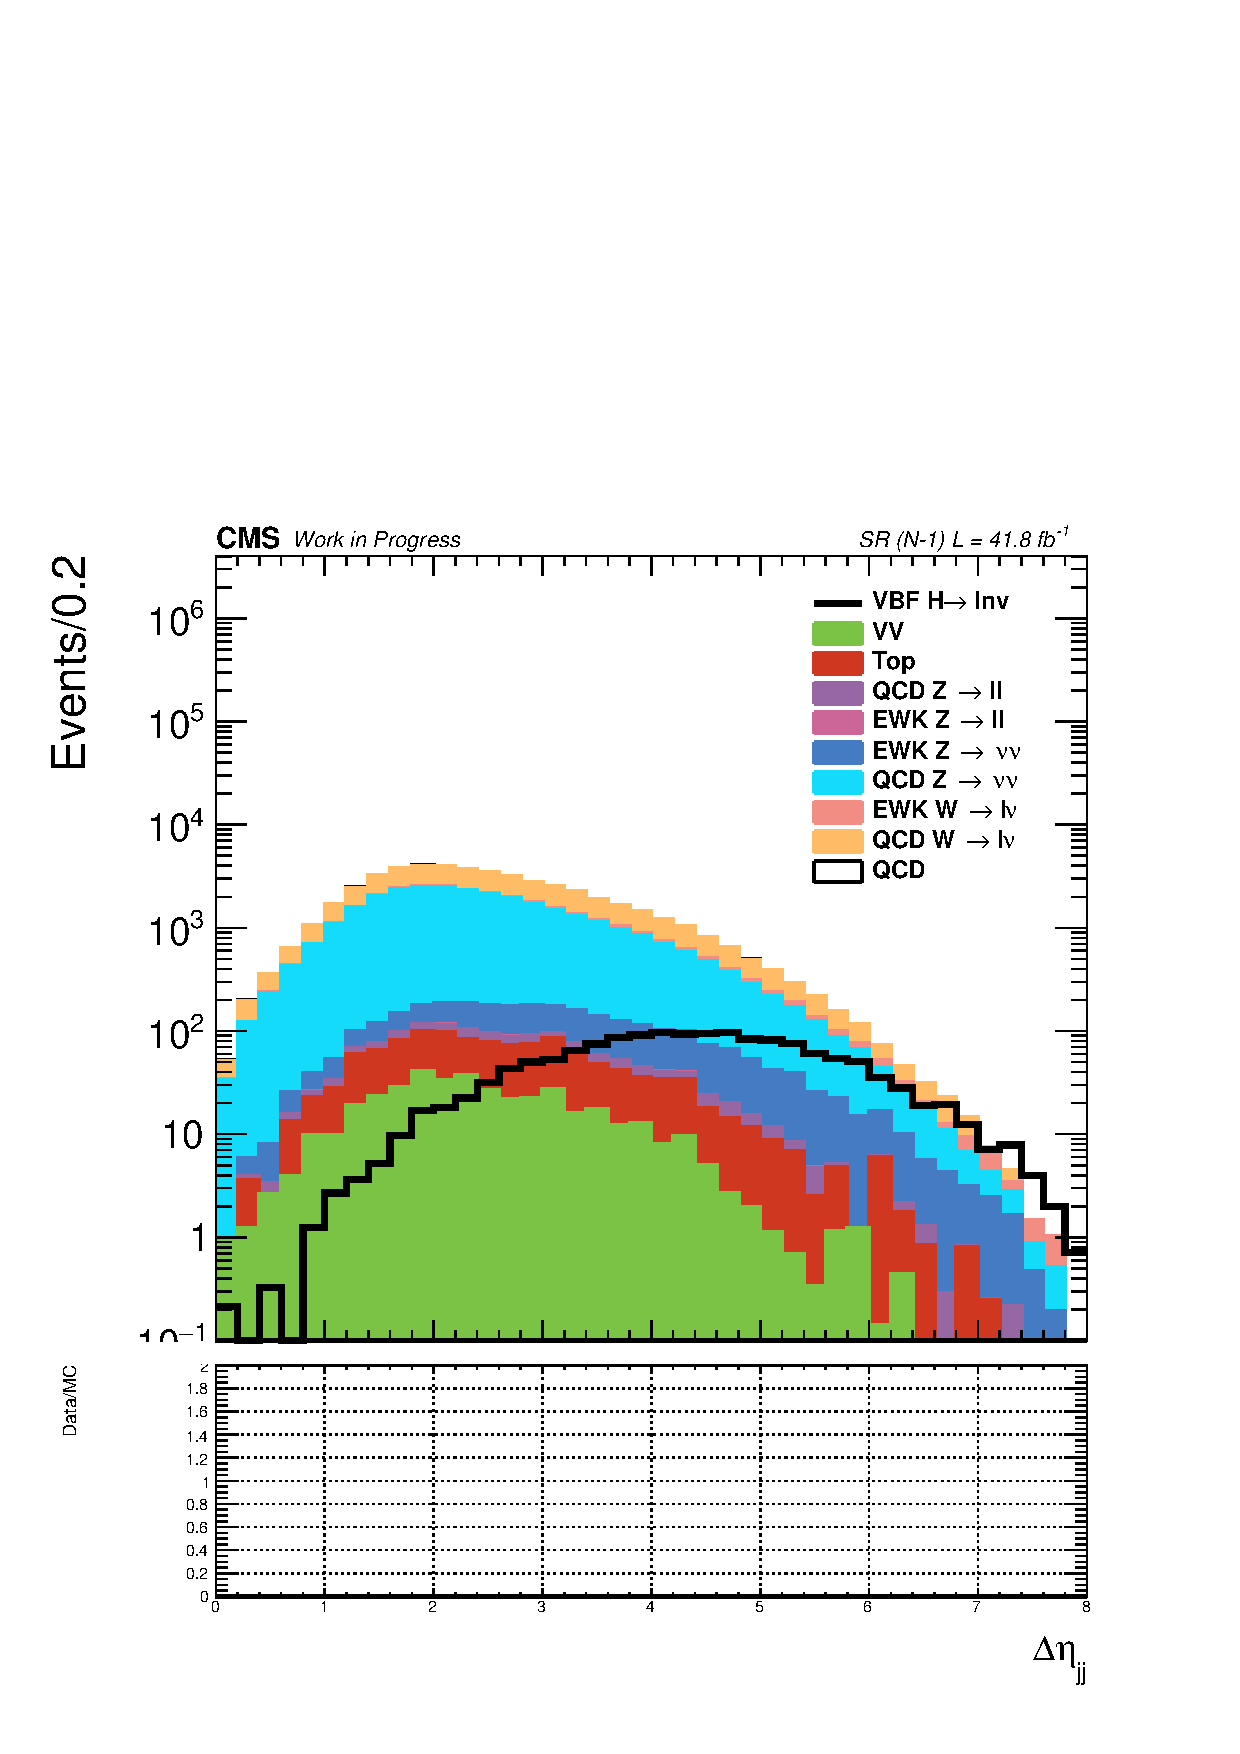
\includegraphics[width=0.49\textwidth]{Analysis_strategy/Nminus1/leading_dEtajj_nminus1_log.pdf}
    }
    \subfigure[$\Delta \phi_{jj}$]{
    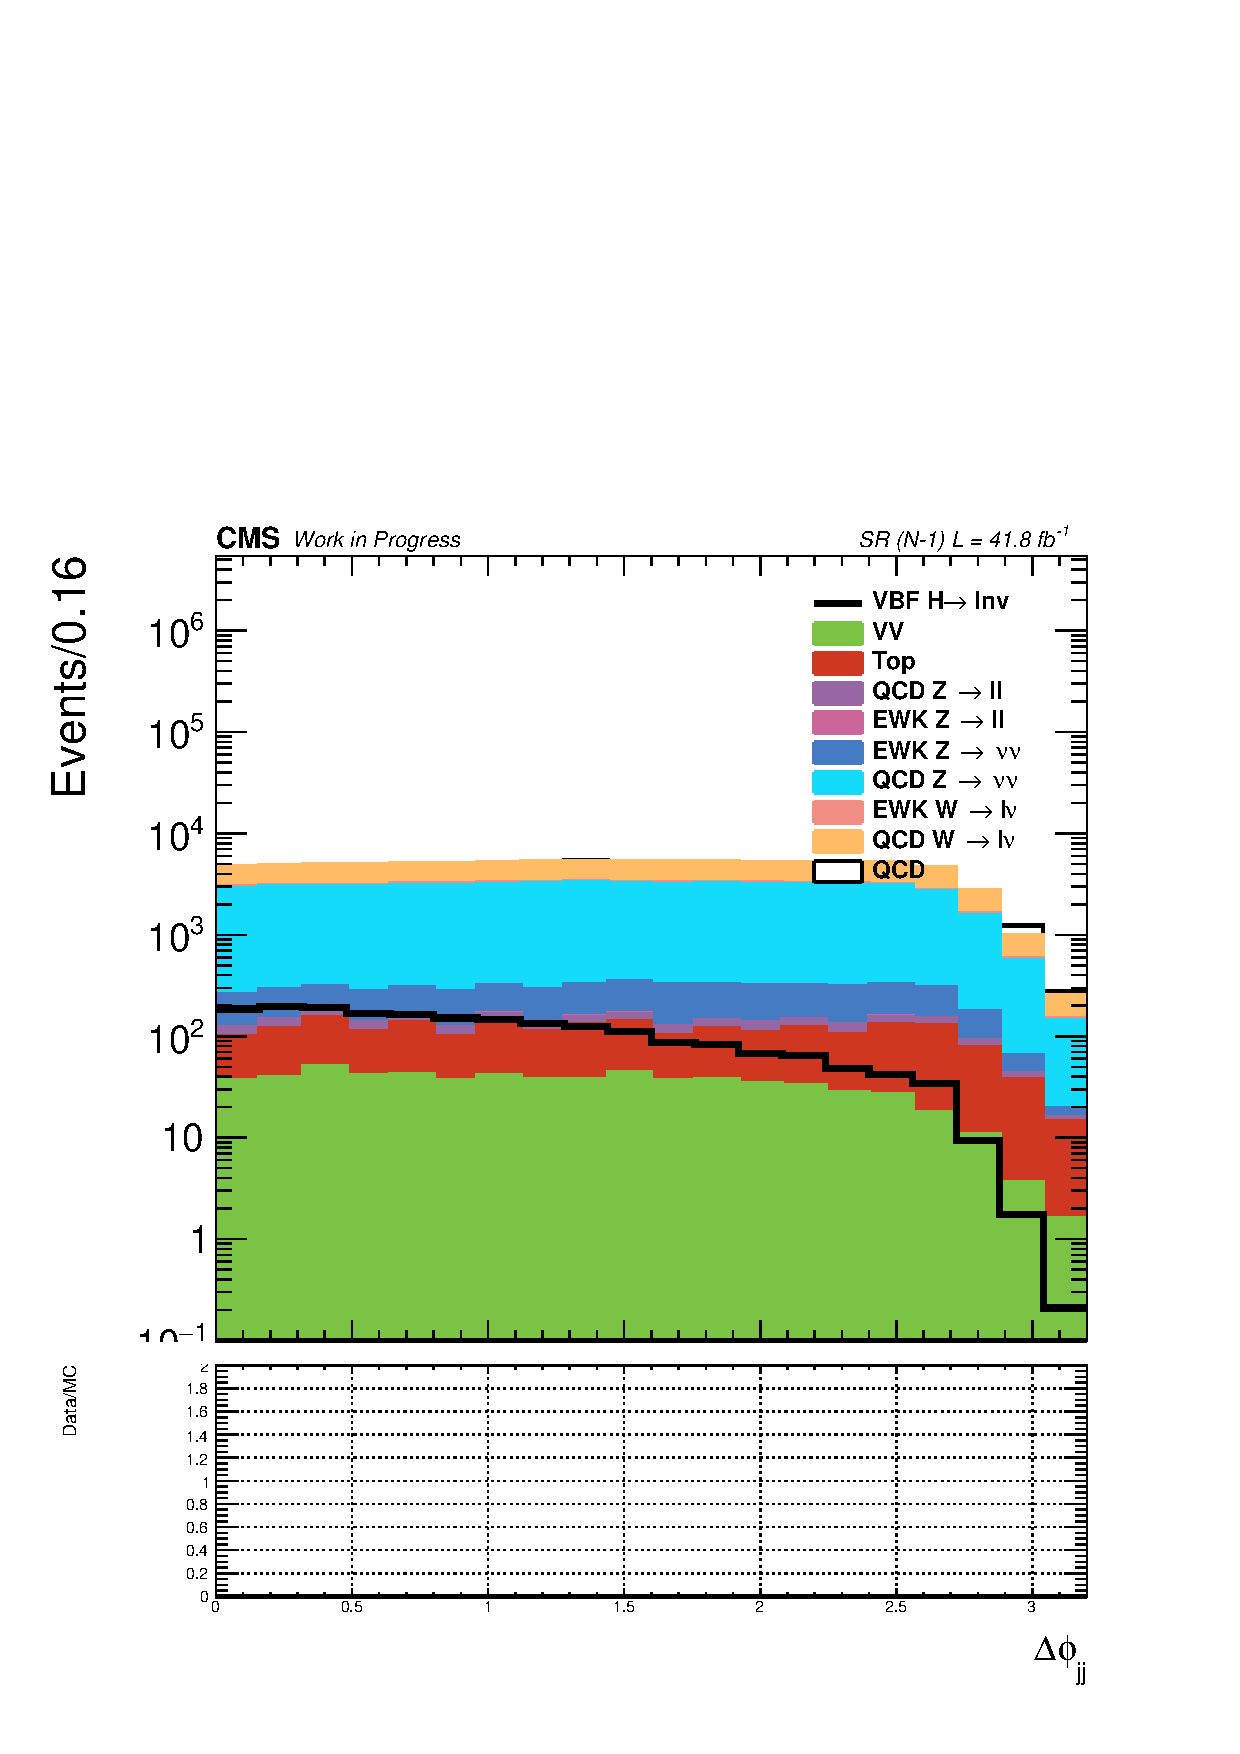
\includegraphics[width=0.49\textwidth]{Analysis_strategy/Nminus1/leading_dPhijj_nminus1_log.pdf}
    }
    
  \caption{Distributions of $min\Delta\phi(j,E_{T,miss})$, $\Delta \eta_{jj}$ and $\Delta \phi_{jj}$ variables in the SR, for the MTR category after the N-1 selection, representing the 2017 era.}
  \label{fig:sr_n-1_shapes_1}
\end{figure}


\begin{figure}[htbp]
  \centering
      \subfigure[$E_{T,miss}$]{
    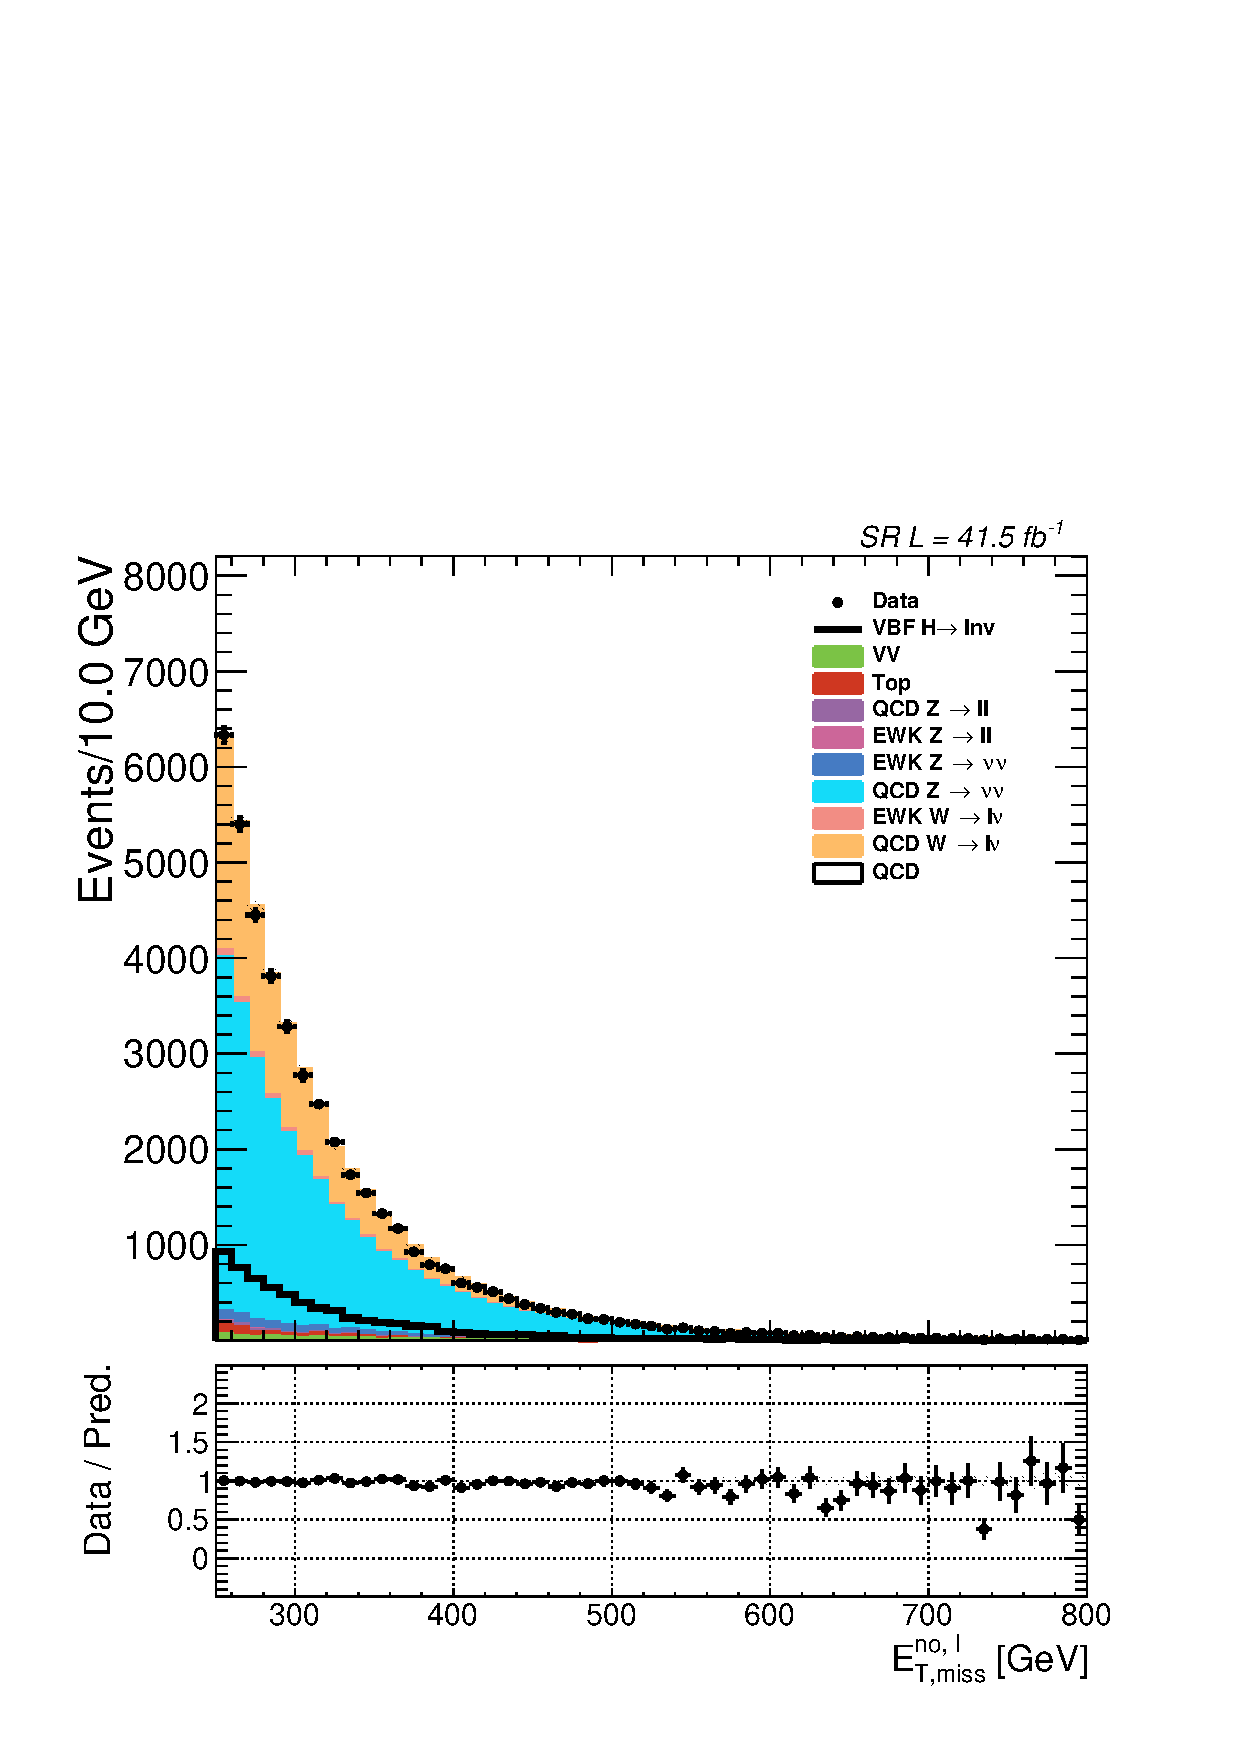
\includegraphics[width=0.49\textwidth]{Analysis_strategy/MTR_2017_SR/MetNoMu.pdf}
    }
    \subfigure[$M_{jj}$]{
    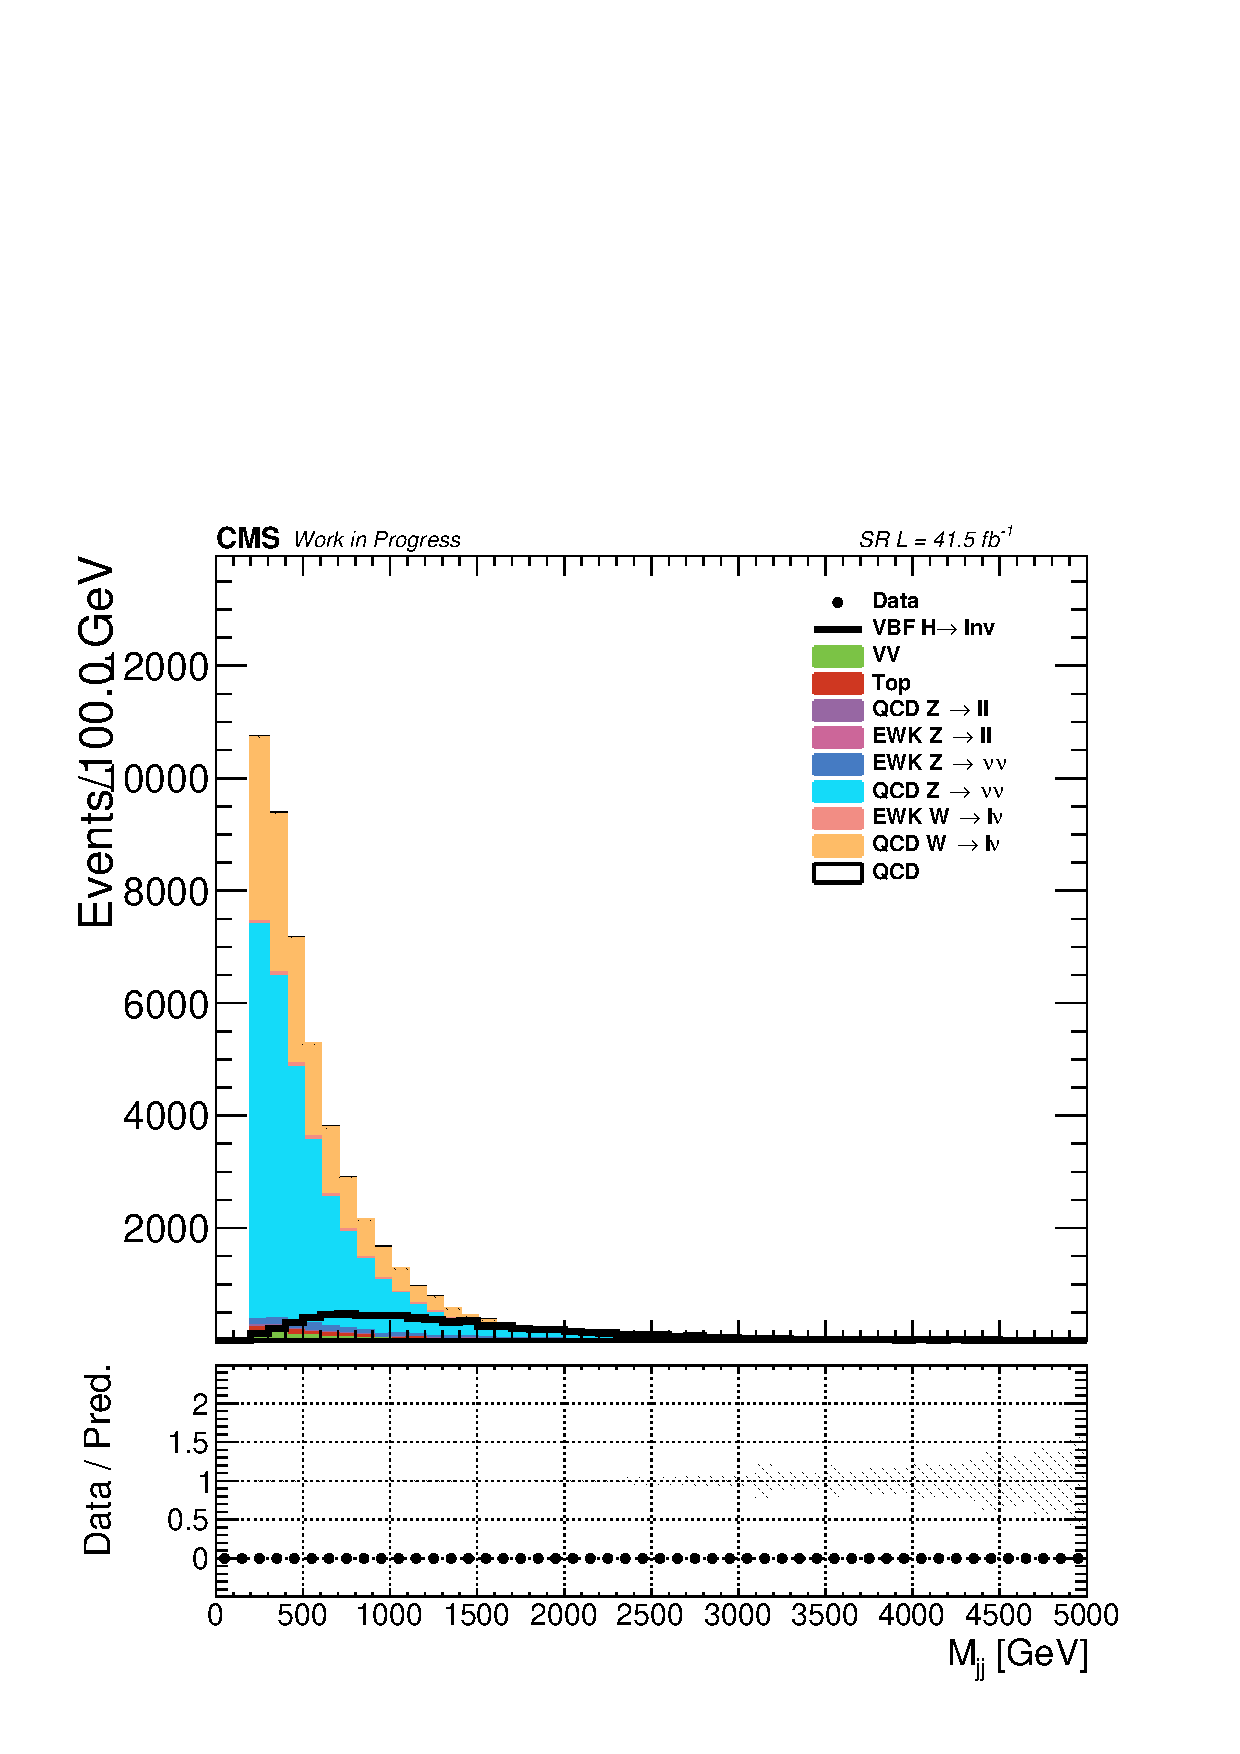
\includegraphics[width=0.49\textwidth]{Analysis_strategy/MTR_2017_SR/leadingJet_mjj.pdf}
    }\\
    \subfigure[$p_{T,j1}$]{
    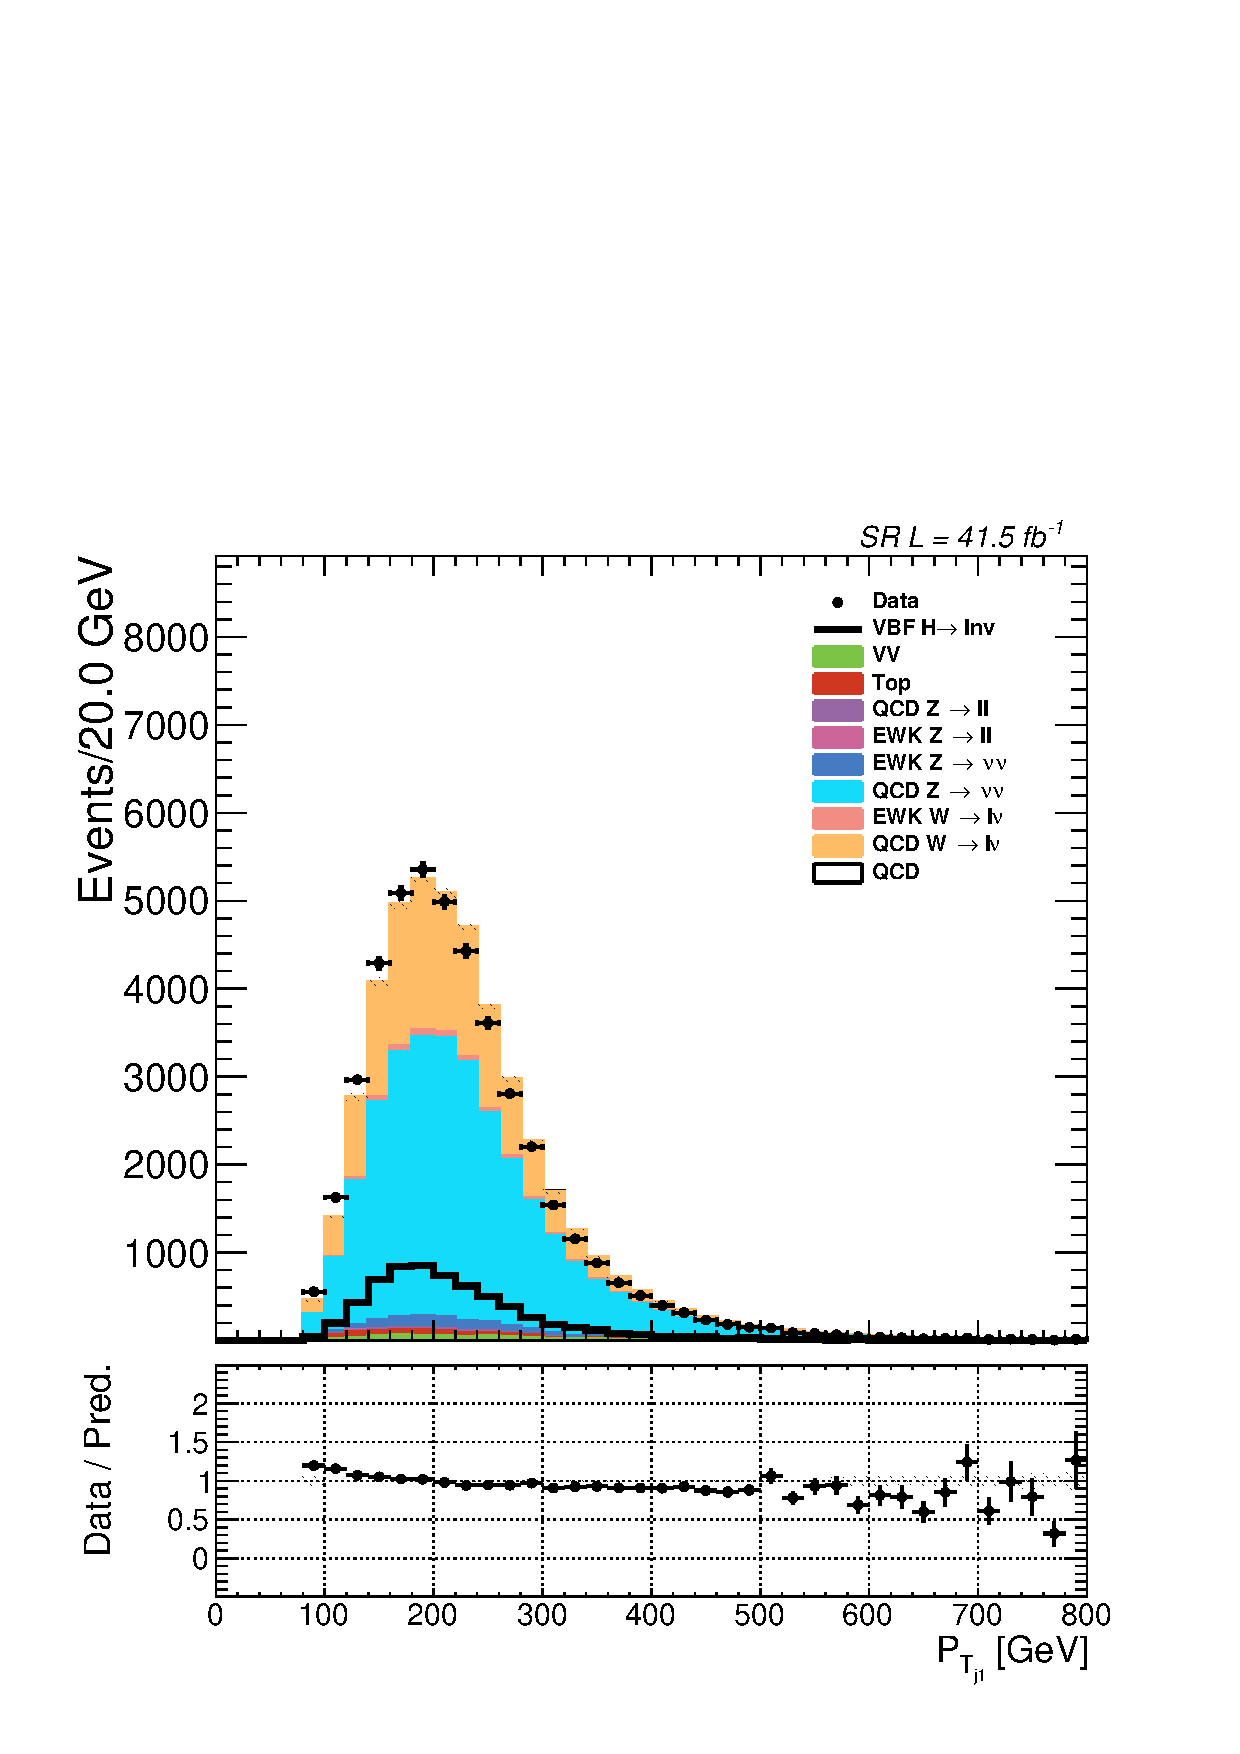
\includegraphics[width=0.49\textwidth]{Analysis_strategy/MTR_2017_SR/Leading_jet_pt.pdf}
    }
    \subfigure[$p_{T,j2}$]{
    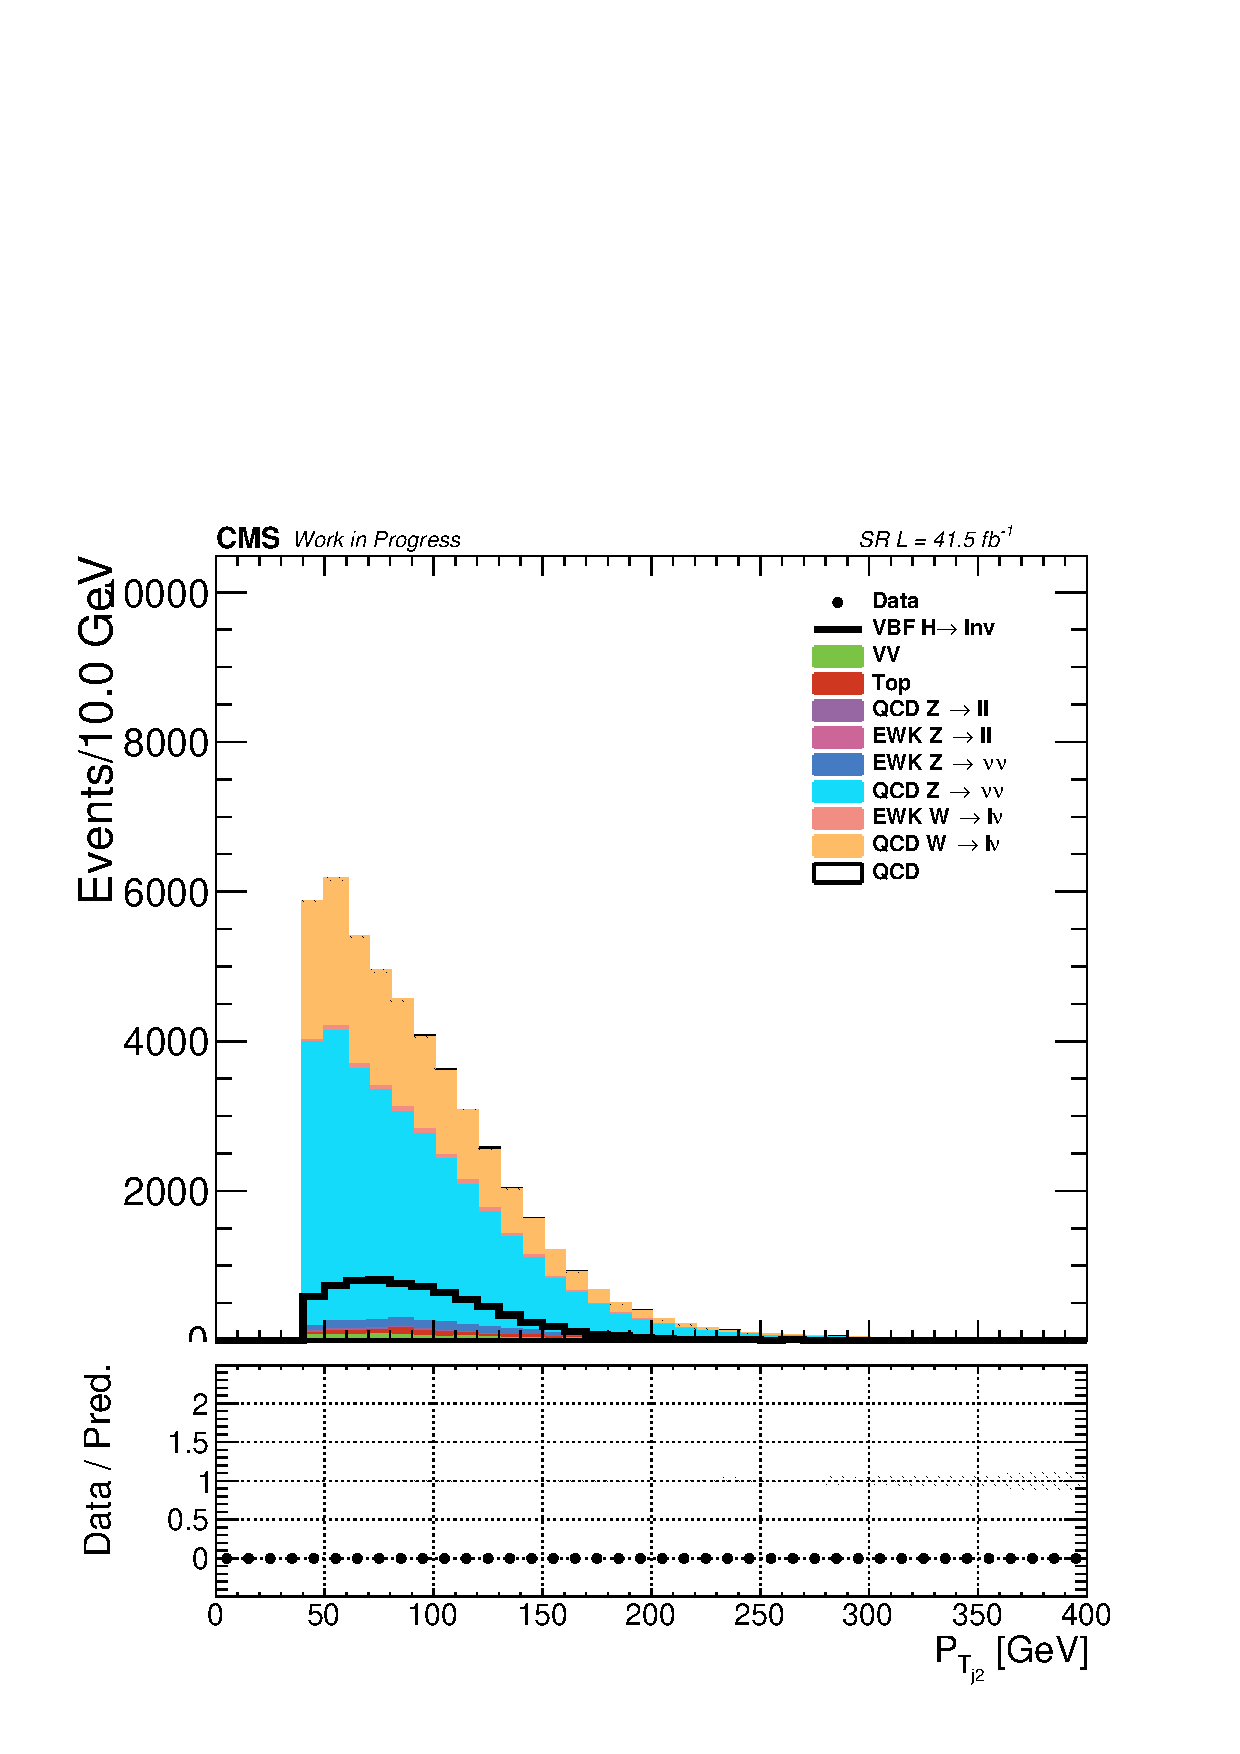
\includegraphics[width=0.49\textwidth]{Analysis_strategy/MTR_2017_SR/Subleading_jet_pt.pdf}
    }
  \caption{Distributions of $E_{T,miss}$, $M_{jj}$, $p_{T,j1}$ and $p_{T,j2}$ variables in the SR after the full MTR selection, representing the 2017 era.}
  \label{fig:sr_n-1_shapes_2}
\end{figure}







\subsection{VBF Trigger category}
\label{subsec:vtr_selection}
\hspace{10pt} Continuing the narrative started in Section~\ref{sec:vbf_trgger}, the main focus of this section is going to be the creation of a new analysis category designed to select the phase space of interest that was overlooked by the MTR category. Following the, previously discussed, blueprint for the MTR category, there is an opening to form a category that will be orthogonal to it. One way to look for its basis is to start from the comparison of performances of both trigger groups and picking an $E_{T,miss}$ range which is outside the MTR threshold, in which VBF triggers perform better than the MTR forming ones. 

\hspace{10pt} As it will be explained in Section~\ref{sec:vbf_trigger_performance}, this study results in a category formed within the $[160,250)~$GeV range of the $E_{T, miss}$ variable. In order to follow the logic deployed at the trigger level, the choice of jets at the analysis level is again based on the dijet pair which yields the largest invariant mass in the event. In retrospect, this choice follows the equivalent procedure to the one presented in Section~\ref{sec:vbf_implementation}. The jets entering the computation are required to have $p_T>$~40~GeV in order to mimic the trigger logic, while the slightly larger threshold is used to account for subtle differences between the HLT and offline jets. Upon constructing the dijet object and optimising the selection based on the trigger performance, thresholds on the values of the dijet mass and transverse momentum of the two jets were set. These selection requirements are then used to form the VTR category and are summarised in Table~\ref{tab:selection_vtr}.


\begin{table}[htbp]
\centering
%\small
\begin{tabular}{lcc}
    Variable                           & Selection                       & Target background \\
    \hline
     & & \\
    $\mu$ ($e$) veto               & $p_T > 10$~GeV,~$|\eta| < 2.4 (2.5)$  & $Z(ll)$~+jets,~$W(l\nu)$~+jets \\
    $\tau$ lepton veto                 & $p_T > 20$~GeV,~$|\eta| < 2.3$        & $Z(ll)$~+jets,~$W(l\nu)$~+jets  \\
    $\gamma$ veto                        & $p_T > 15$~GeV,~$|\eta| < 2.5$        & $\gamma$~+jets \\
    B jet veto                    &  $p_T > 20$~GeV,~$|\eta| < 2.4$  &  Top quark\\
        & & \\
    $E_{T,miss}$                          & $[160,250)$~GeV                          & QCD, top quark, $Z(ll)$~+jets \\
    $min\Delta\phi(j, E_{T,miss})$   &  $ {>} 1.8$ radians               & QCD \\
    $min\Delta\phi(j, E_{T,miss})$   &  $ {>} 0.5$ radians               & QCD \\
        & & \\
    Largest $m_{jj}$                               & ${>}$ 900~GeV  \\       
    $p_{T,j_1}$ and $\eta_{j1}$   & ${>} 140$~GeV and $ |\eta| < 4.7$      & All \\
    $p_{T,j_2}$ and $\eta_{j2}$   & ${>} 70$~GeV and $ |\eta| < 4.7$      & All \\
    $\eta_{j1}\cdot\eta_{j2}$   & ${<}$ 0   & All \\
    $\Delta\eta_{jj}$                            & ${>} 1.0$  \\
    $\Delta\phi_{jj}$                            & ${<} 1.5$  \\
      & & \\
         \hline
\end{tabular}
\caption{Summary of the VTR selection requirements, accompanied with the target background processes affected by them~\cite{note:AN_19_257}.}
\label{tab:selection_vtr}
\end{table}

\hspace{10pt} This approach ensures the "out of the box" orthogonality between two analysis categories. The high thresholds for jet $p_T$ values and the large dijet mass requirement reduce the difference between two choices of VBF jets between categories. The requirements on the $\Delta\eta_{jj}$ and $\Delta\phi_{jj}$ are directly constrained by this, allowing for the usage of the same, previously optimised, requirements from the MTR category.

\hspace{10pt} On the other hand, as this approach follows the logic given by the trigger, it is expected to bring a certain amount of QCD multijet events as well. As seen in the previous section, a good handle for dealing with these processes is given in the form of the $min\Delta\phi(j, E_{T,miss})$ variable. Figure~\ref{fig:VTR_mindphi} shows the distribution of this variable in the VTR SR after the application of a looser ($>0.5$) requirement. It can be seen that values bellow 1.8 are largely background dominated, with the QCD multijet processes leading the way, while being populated with a low yield of signal events, thus motivating a requirement which would remove this region without risking a significant loss in signal acceptance. 

\begin{figure}[htbp]
  \centering
    \subfigure{
    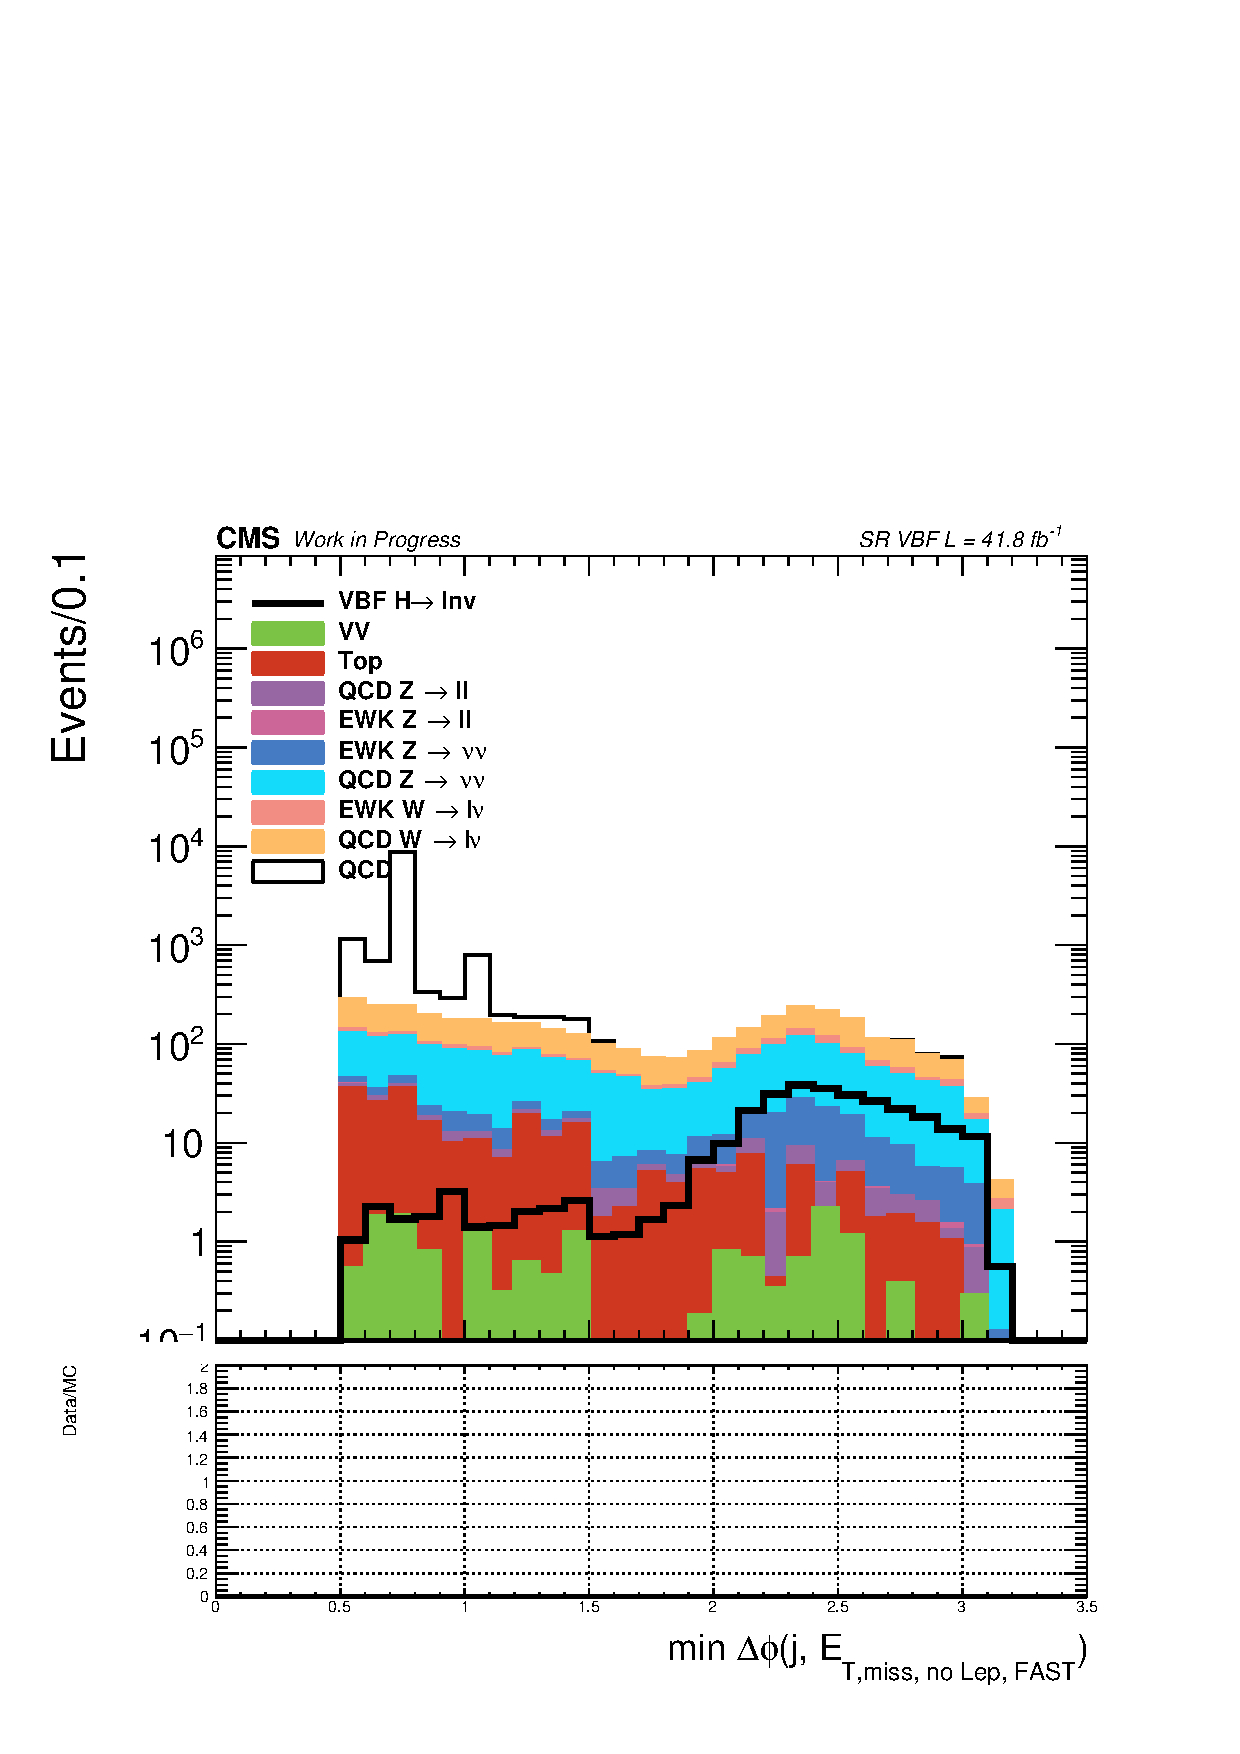
\includegraphics[width=0.49\textwidth]{Analysis_strategy/Nminus1/VTR/MetNoLep_CleanJet_mindPhi_FAST_log.pdf}
    }
  \caption{Distribution of the \mindphi~variable in the SR after the VTR-like selection requirements.}
  \label{fig:VTR_mindphi}
\end{figure}
Figure~\ref{fig:VTR_SR_2017} shows the data to simulation comparisons for a few selected variables after the full VTR selection. A set of dedicated control regions will be created for the VTR category, analogous to the MTR approach, in order to improve the overall data to simulation agreement. In order to efficiently illustrate the discussion given in these two sections, only the 2017 era of data taking was presented for both MTR and VTR categories. Additional set of distributions for VTR category representing the 2018 era is given in Appendix~\ref{app:MTR_2018} alongside their MTR counterparts. 


%first step will be to see how this orthogonality can be achieved on the selection level. Following the trigger turnons given in Figures [TBD] and the definition of the MTR category (introduced in the prvious paragraph), it can be seen that a $E_T^{miss}$ range of $[160,250)~$GeV represents a good requirement that would clearly establish the separation between two categories. Figures [TBD] and [TBD] showcase the Signal Region for the VTR category taking into account two selection options showcased in Section~\ref{sec:triggers}. Based on the conclusion of that section (and also taking into account that both options give similar event yields), option B, where the HLT selection logic is followed, will be used to define the VTR category. Additionally a higher requirement on $min\Delta\phi(jet,~E_T^{miss,~no~lep})>1.8$ has been added to reduce the contribution from multijet processes. 




\begin{figure}[htbp]
  \centering
    \subfigure[$\Delta \eta_{jj}$]{
    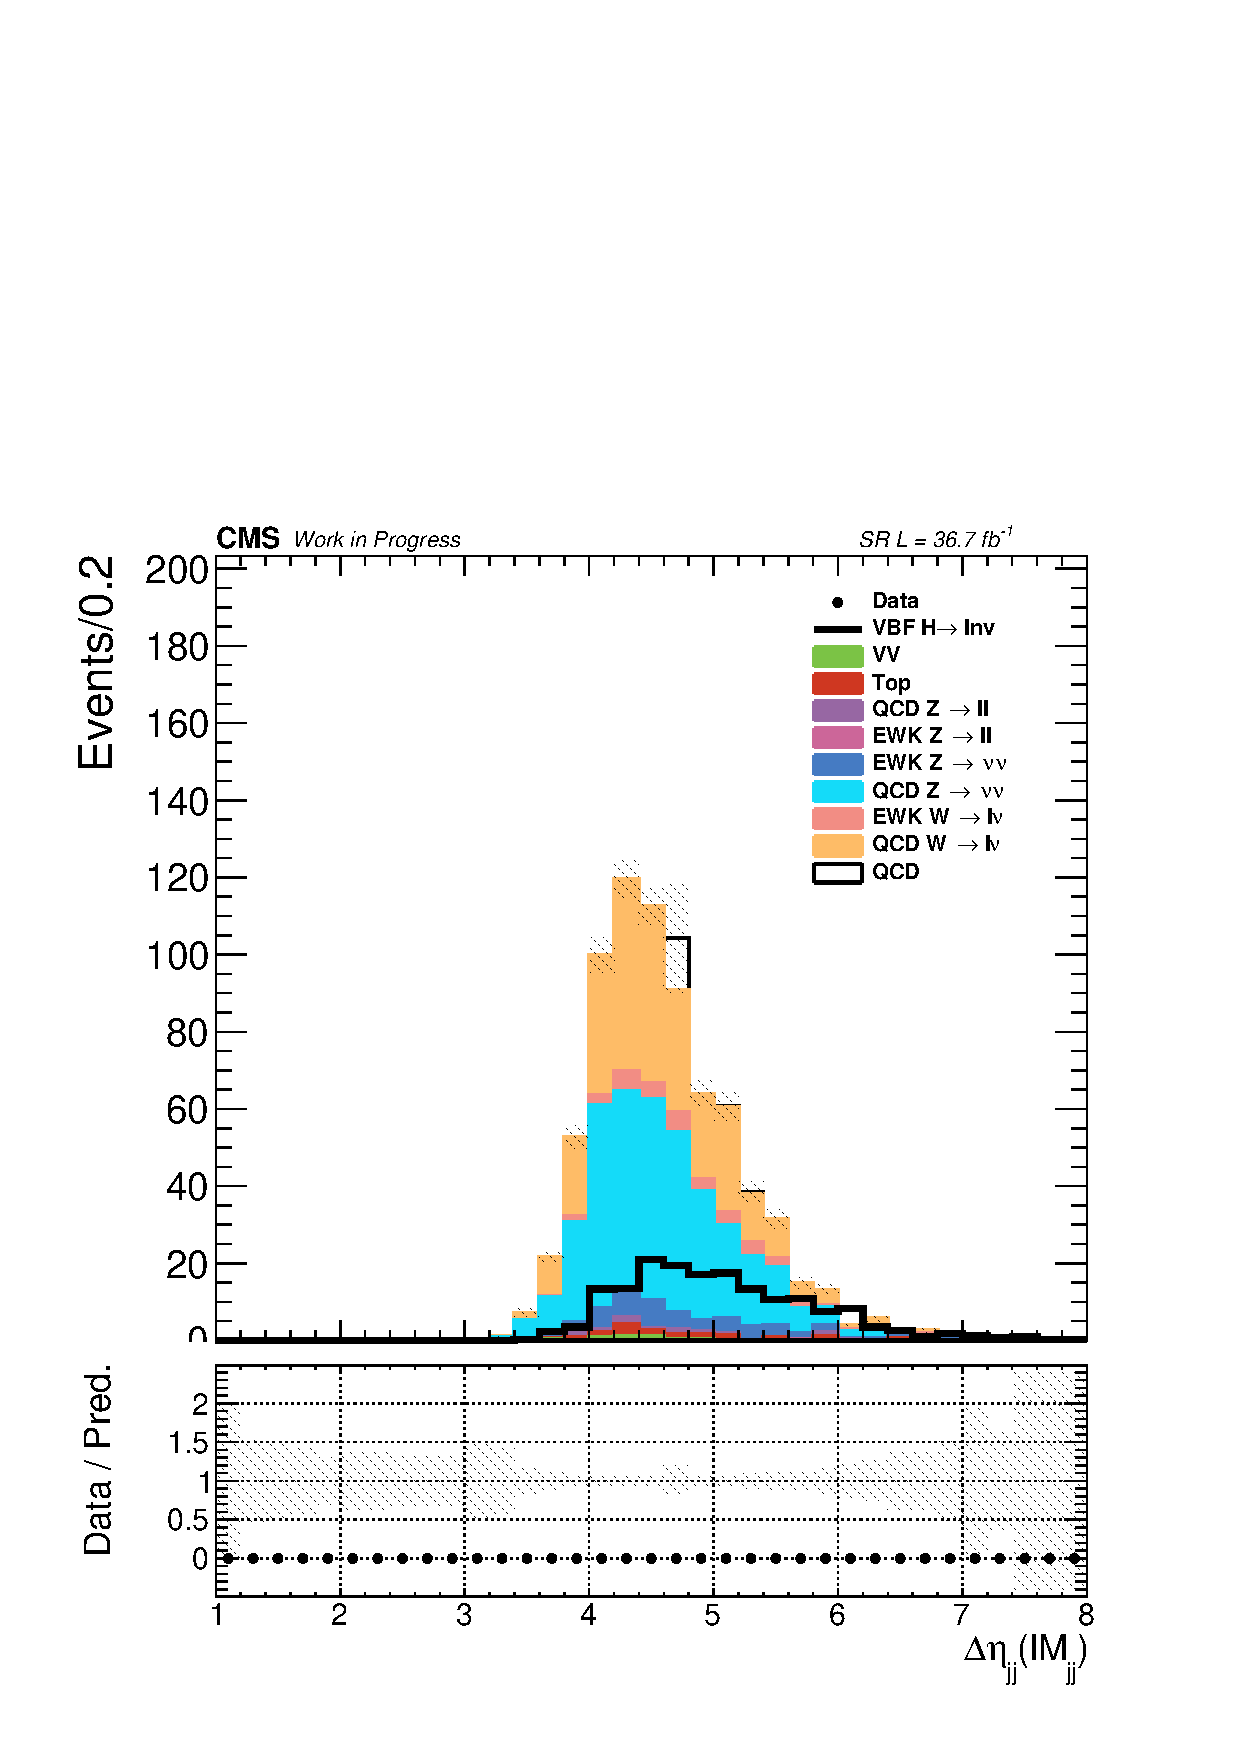
\includegraphics[width=0.49\textwidth]{Analysis_strategy/VTR_2017_SR/lMjj_leading_dEtajj.pdf}
    }
    \subfigure[$\Delta \phi_{jj}$]{
    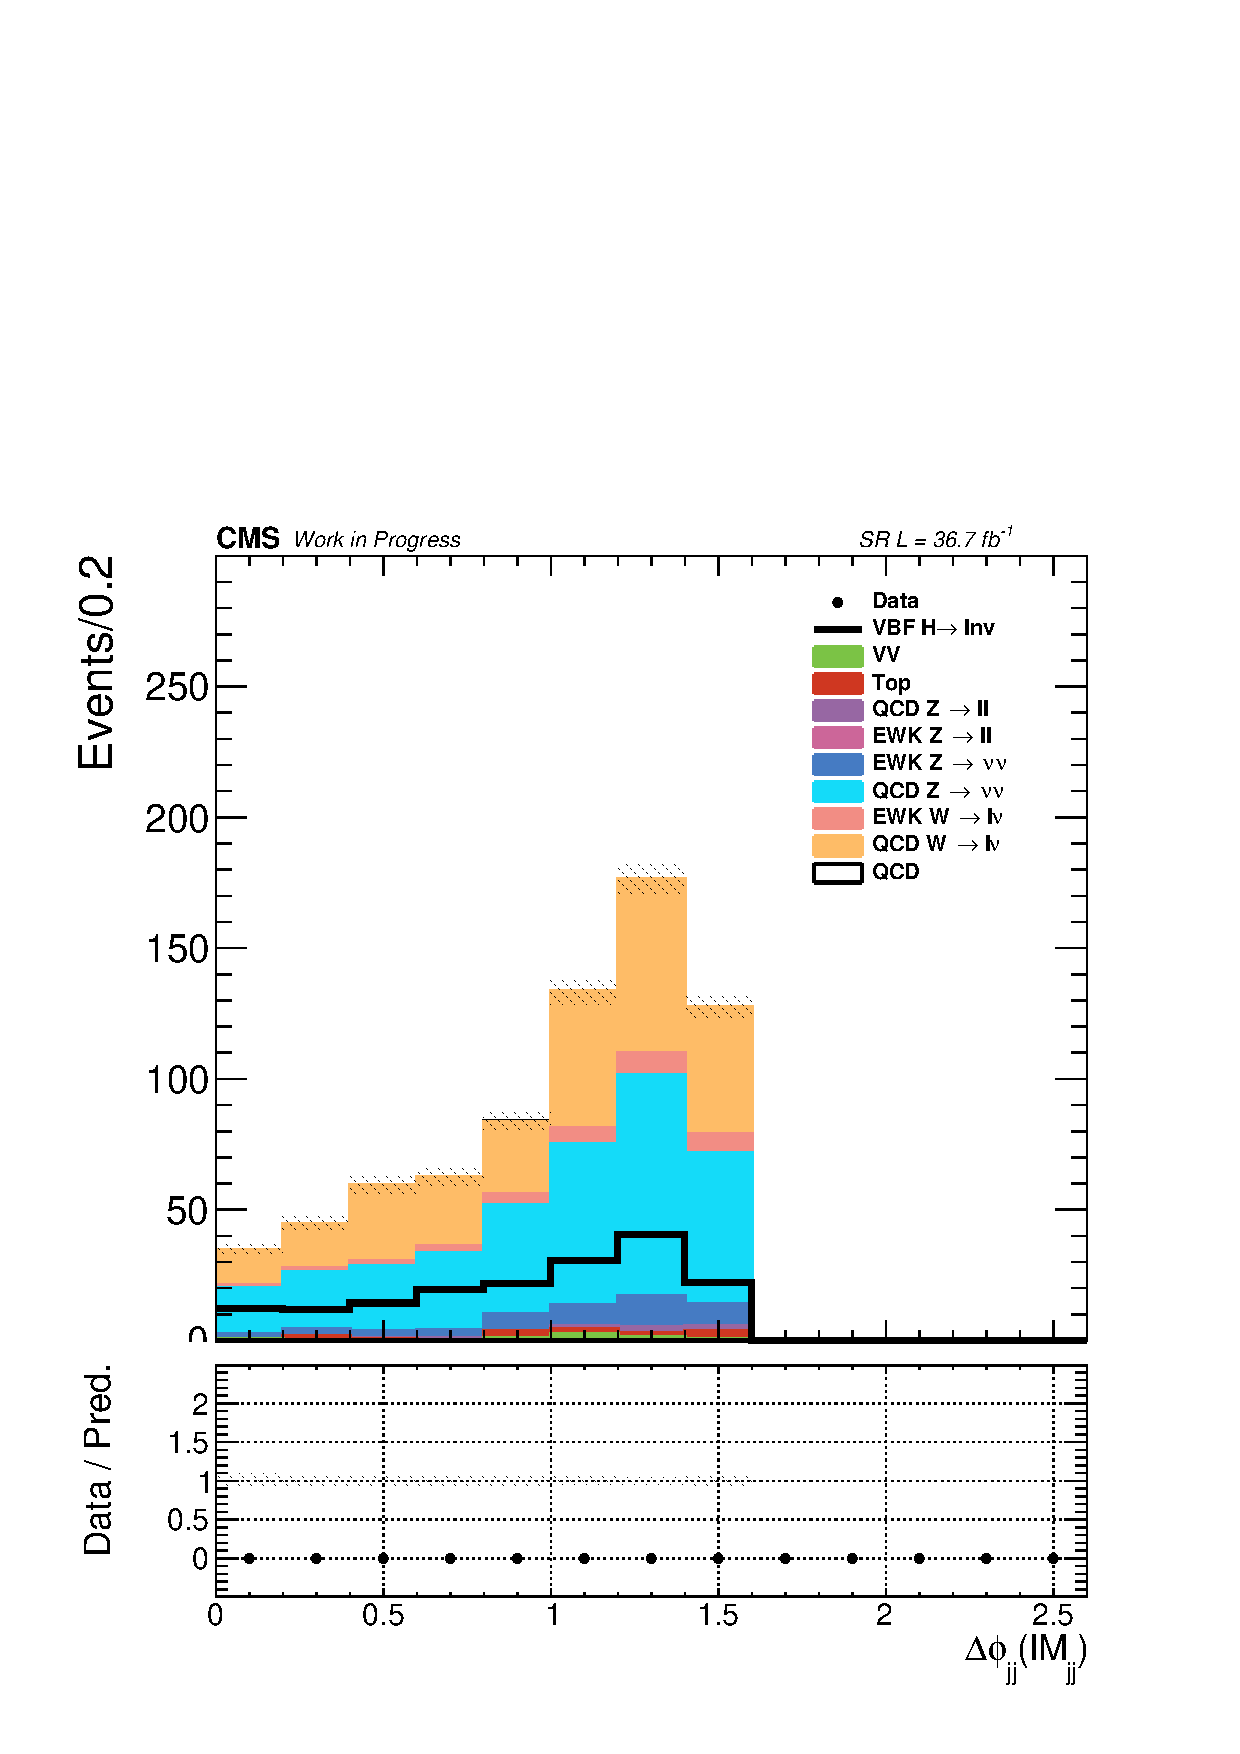
\includegraphics[width=0.49\textwidth]{Analysis_strategy/VTR_2017_SR/lMjj_leading_dPhijj.pdf}
    }\\
    \subfigure[$m_{jj}$]{
    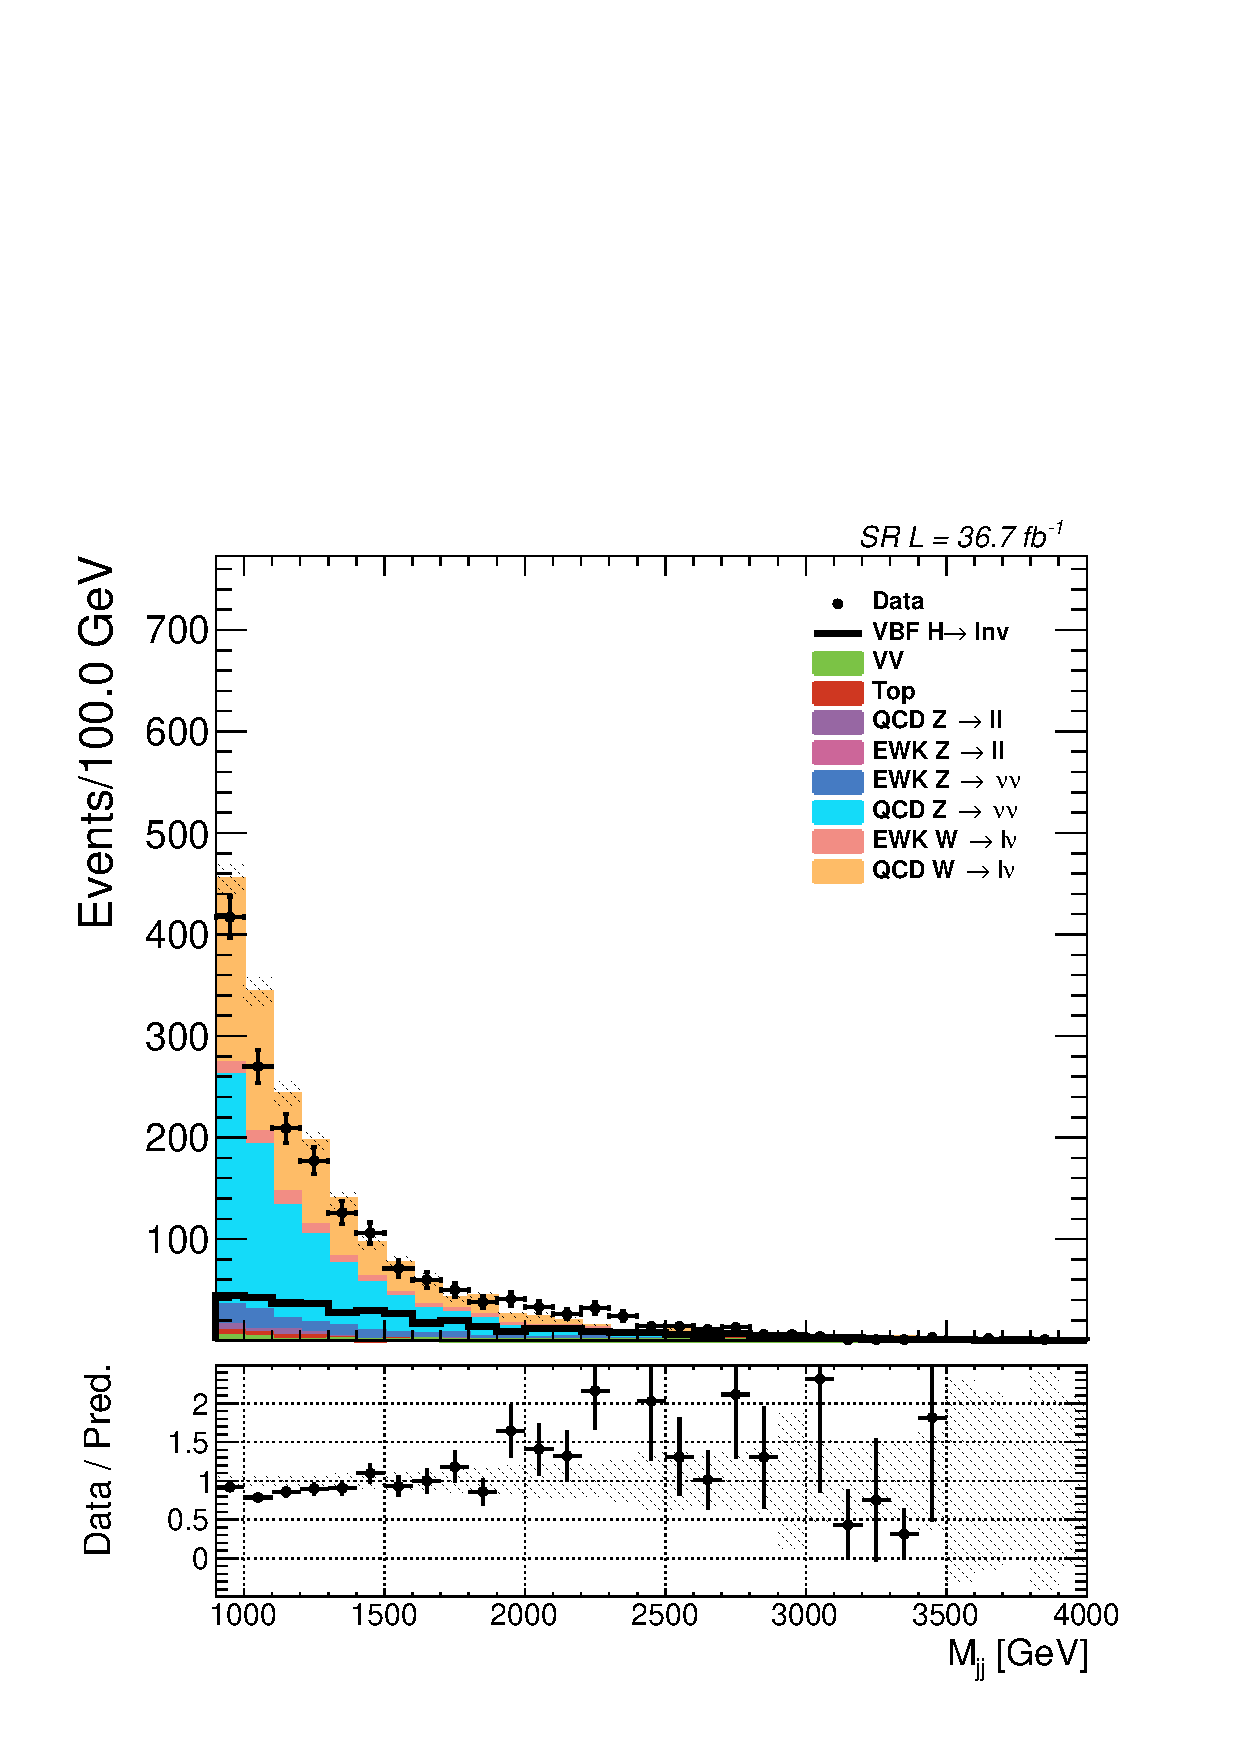
\includegraphics[width=0.49\textwidth]{Analysis_strategy/VTR_2017_SR/lMjj.pdf}
    }
    \subfigure[$E_{T,miss}$]{
    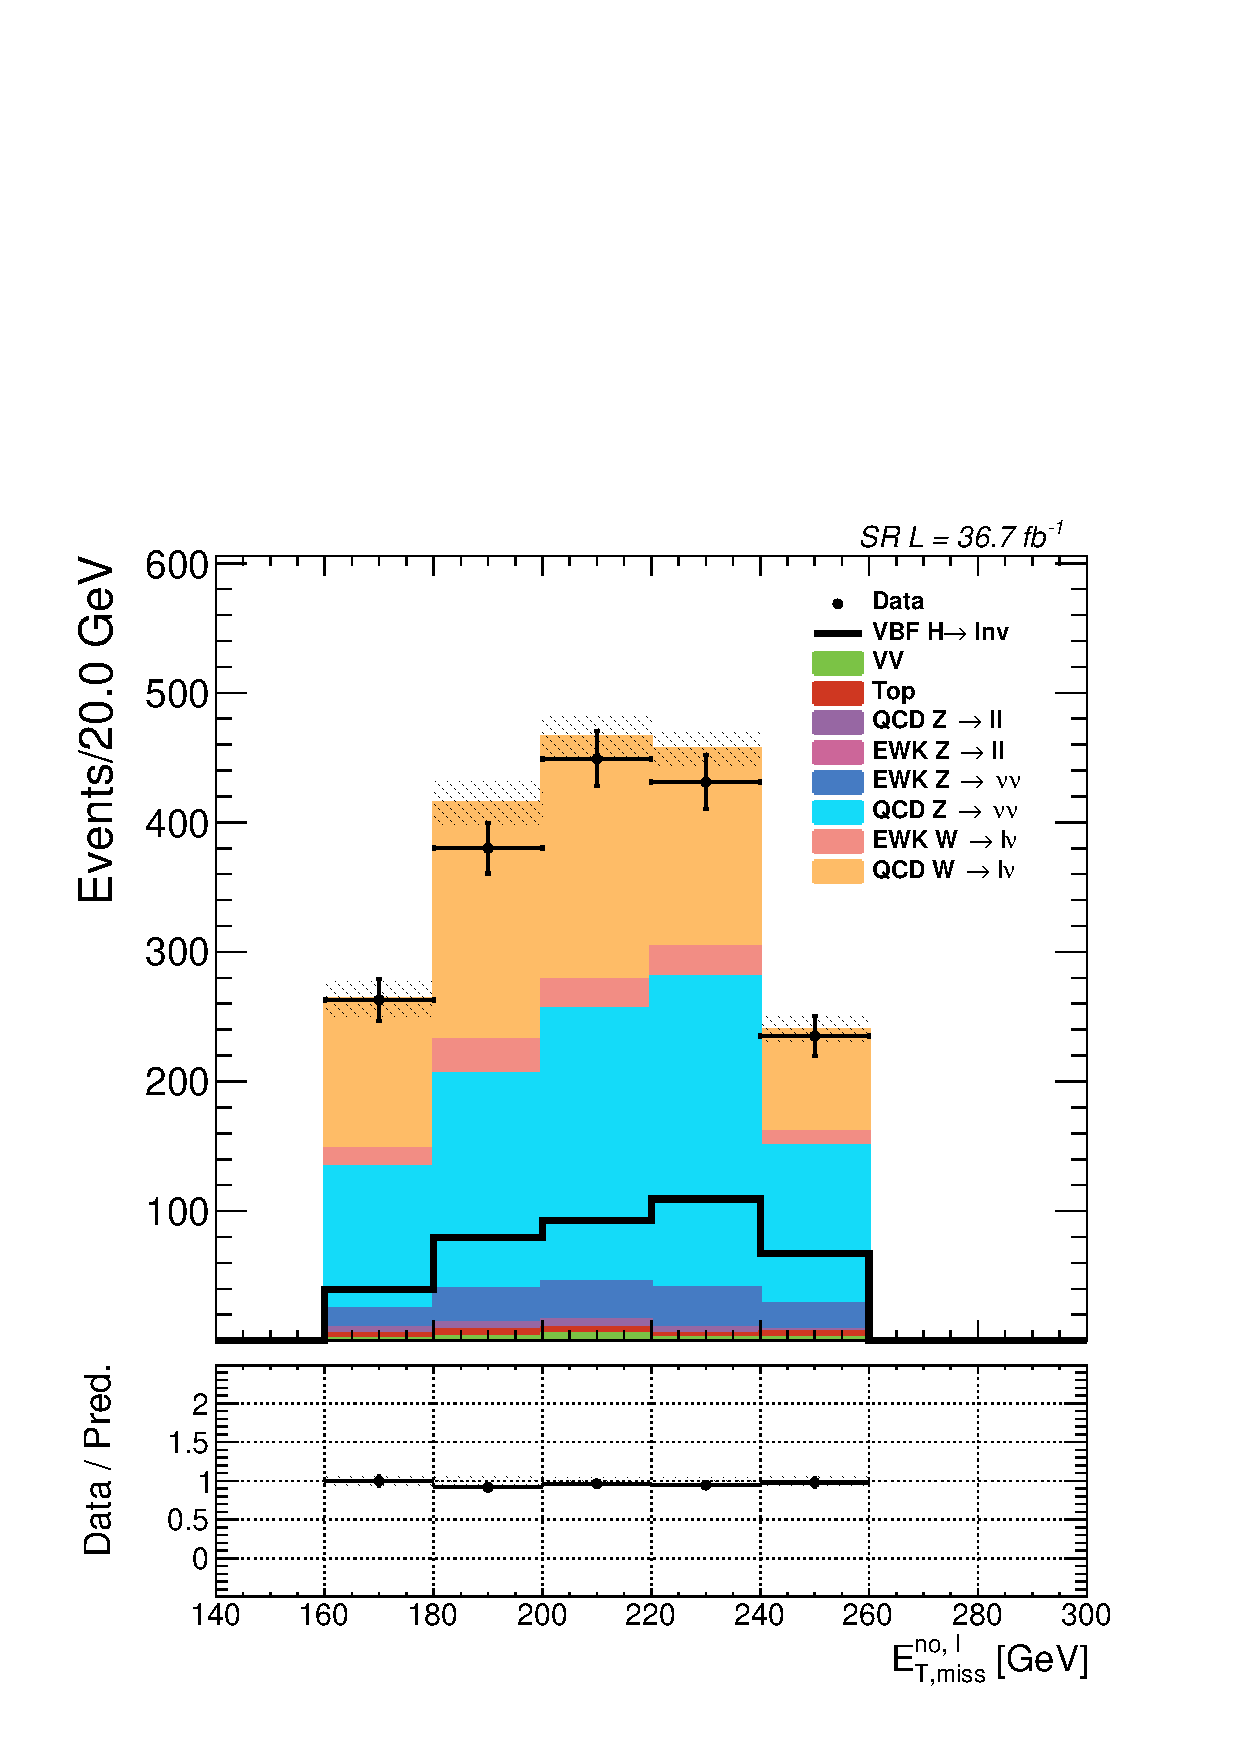
\includegraphics[width=0.49\textwidth]{Analysis_strategy/VTR_2017_SR/MetNoMu.pdf}
    }
  \caption{Distributions of $\Delta \eta_{jj}$, $\Delta \phi_{jj}$, $m_{jj}$ and $E_{T,miss}$ variables int the signal region after the full VTR selection, representing the 2017 era.}
  \label{fig:VTR_SR_2017}
\end{figure}


\section{Trigger Performance}

\hspace{10pt} The following sections focus on the performance of the HLT algorithms used in this analysis. These paths can be split into two groups based on their usage: the signal/muon region and the electron region forming triggers. The added benefit of the signal triggers (listed in Tables~\ref{tab:hlt_rates} and~\ref{tab:metmht}) comes from the fact that they are built by adding conditions on $E_{T, miss}^{~no, \mu}$ (as seen in the diagram presented in Figure~\ref{fig:VBF_HLT}). The $\vec{p}_{T, miss}^{~no, \mu}$ vector, whose intensity is represented by $E_{T, miss}^{~no, \mu}$, is defined by adding the transverse momentum of muon objects back into the $\vec{p}_{T, miss}$ computation. This can be expressed as:
\begin{equation}
  \vec{p}_{T, miss}^{~no, \mu} = \vec{p}_{T, miss} + \sum_i \vec{p}_{T,\mu_i},
\end{equation}
where the sum goes over all muon objects. Such definition of the missing energy is equivalent to the standard $E_{T, miss}$ for the SR, due to the usage of a muon veto. This re-definition extends the usability of aforementioned trigger algorithms, which can now be used to select events entering muon regions (more details about these specialised regions are given in Section~\ref{sec:control_regions}). For the regions containing electron objects, a combination of electron and photon triggers is used. The addition of photon triggers was performed in order to achieve better statistics in these regions (which will benefit the double electron region, due to its tight requirements). The complete list of HLT paths used in this analysis (and the corresponding L1 seeds used as input) is given in Table~\ref{a_tab:triggers}.

\subsection{Performance of $E_T^{miss}$ and $H_T^{miss}$ based triggers}
\label{subsec:mtr_triggers}
\hspace{10pt} Following the ordering used in the previous section, the first topic of discussion is going to be the performance of triggers used to form the MTR category. Listed in Table~\ref{tab:metmht}, they are represented by a set of selection requirements on $E_{T,miss}^{~no,\mu}$ and $H_{T,miss}^{no,~mu}$ variables at the HLT stage. This section is going to summarize the study of their performance during the 2017 and 2018 era of data collection. It is going to be based around the analysis selection requirements for the MTR category (as shown in Table~\ref{tab:selection_mtr}), presenting the motivation behind the $E_{T,miss}$ threshold (which is set with respect to the overall performance). More details about the choice of the selection itself can be found in Section~\ref{subsec:vbfselection}.

\begin{table}[htbp]
\centering
%\small
\begin{tabular}{l|c}
\hline\hline
Era & Trigger name                                               \\ \hline
\multirow{4}{*}{2017 \& 2018} &\\
                      &\texttt{HLT\_PFMETNoMu120\_PFMHTNoMu120\_IDTight\_PFHT60}\\
                        &\texttt{HLT\_PFMETNoMu120\_PFMHTNoMu120\_IDTight}\\ 
                        &\\\hline
\hline\hline
\end{tabular}
\caption{List of $E_{T,miss}$ and $H_{T,miss}$  triggers used in the analysis. Conventional names are used to describe the HLT level requirements imposed on the variables, with them being: $E_{T,miss}^{~no,\mu}>$ 120~GeV and $H_{T,miss}^{~no,\mu}>$ 120~GeV (with the addition of the $H_T>$~60~GeV requirement for the backup path).  \label{tab:metmht}}
\end{table}
\hspace{10pt} During the 2017 era of data taking, a special, control, version of main $E_{T,miss}$ path had to be introduced, as the main one was prescaled due to problems which led to the drastic increase of its rate. The origin of this problem is connected to the same issues plaguing the L1 VBF seed as explained in Section~\ref{sec:vbf_trgger}. This has resulted in the inclusion of the additional $H_T>$60~GeV requirement at the trigger level. This issue was quickly mitigated in 2017 by applying slightly higher thresholds on the input L1 seeds, thus reducing the amount of rate brought by the trigger. This backup path was kept for the entirety of 2018 era, but with certain modifications applied to its input. As it was noticed that it brought an efficient reduction in rate when used as a backup, it was redeployed with lower requirements applied to the input L1 seeds, allowing for it to be used alongside the main path in the analysis.

\hspace{10pt} The general approach when measuring efficiencies for both eras is to form dedicated regions in which the actuall measurement will be performed. For this study this is done by using a slightly modified definition of a single muon control region. As described in Section~\ref{sec:single_muon}, this modified the muon veto condition by asking for the existence of exactly one muon object in the event which passes the tight conditions. For the measurement itself, a control HLT path is being used (\texttt{HLT\_IsoMu27}), which represents a single muon trigger looking for muon objects with $p_T>$27~GeV which pass the isolation requirement at the HLT level. In order to ensure that the study is performed in a region of high control trigger efficiency (on the trigger "plateau"), a requirement $p_{T,\mu}>30$~GeV is imposed on the selected tight muon. The efficiency measurement is presented in terms of $E_{T,miss}^{~no,\mu}$ bins and defined as:

\begin{equation}
\text{Efficiency} = \frac{(\text{Passing analysis selection requirements})~and~(\text{HLT triggered})}{\text{Passing analysis selection requirements}},
\end{equation}

The efficiency of the logical OR of the two HLT paths is measured both in data and simulation, while the resulting difference is being used as a scale factor which is applied, in main analysis, to simulation samples on an event by event basis (as described in Section~\ref{sec:object_corr}). Inputs for these measurements are formed from the muon enriched dataset (Single Muon PD) and the QCD W+jets simulaton samples, representing the dominant SM process in this region. Figure~\ref{fig:metmht_effs} presents the resulting efficiencies, with the corresponding scale factors, for both 2017 and 2018 eras.

\begin{figure}[htbp]
  \centering
    \subfigure[2017]{
    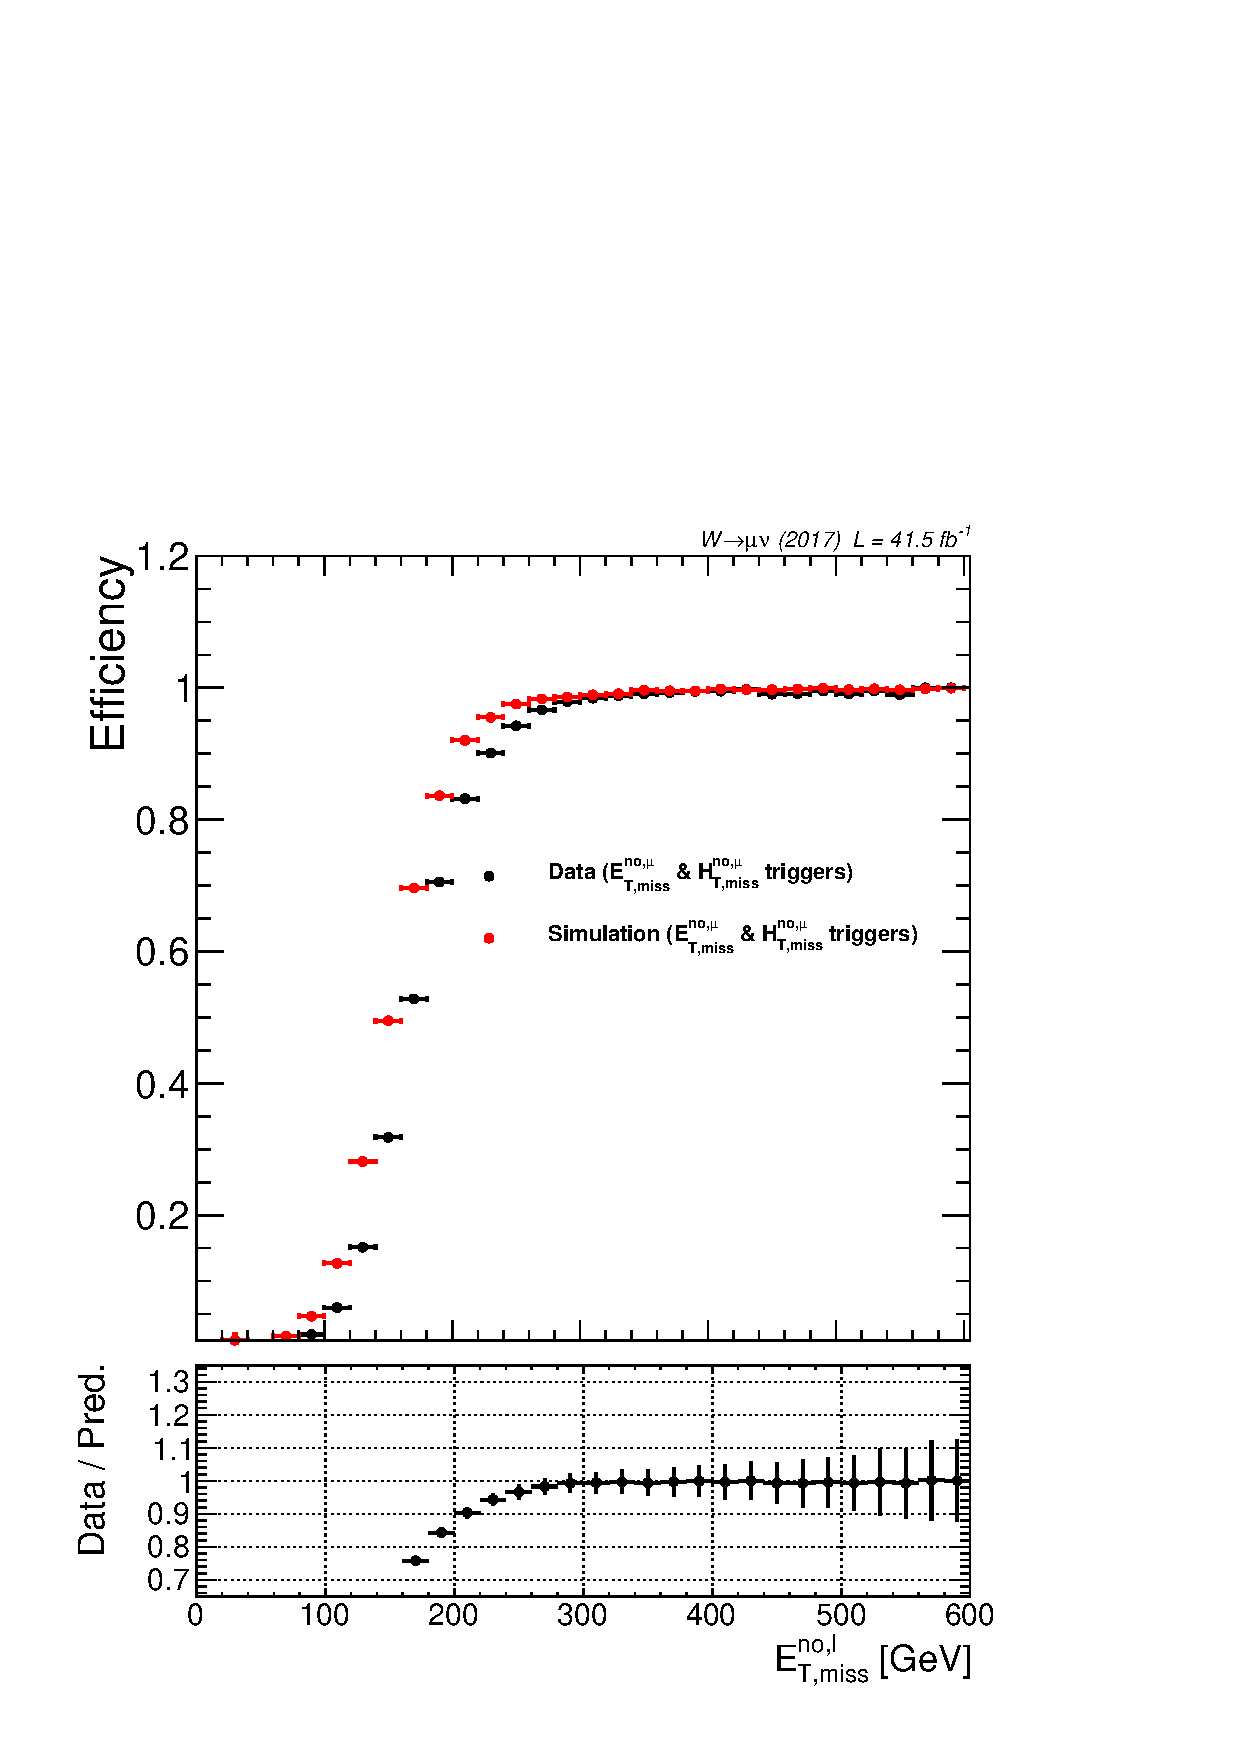
\includegraphics[width=0.45\textwidth]{Analysis_strategy/METMHT_eff/MetNoMuMETMHT_2017.pdf}
    }
    \subfigure[2018]{
    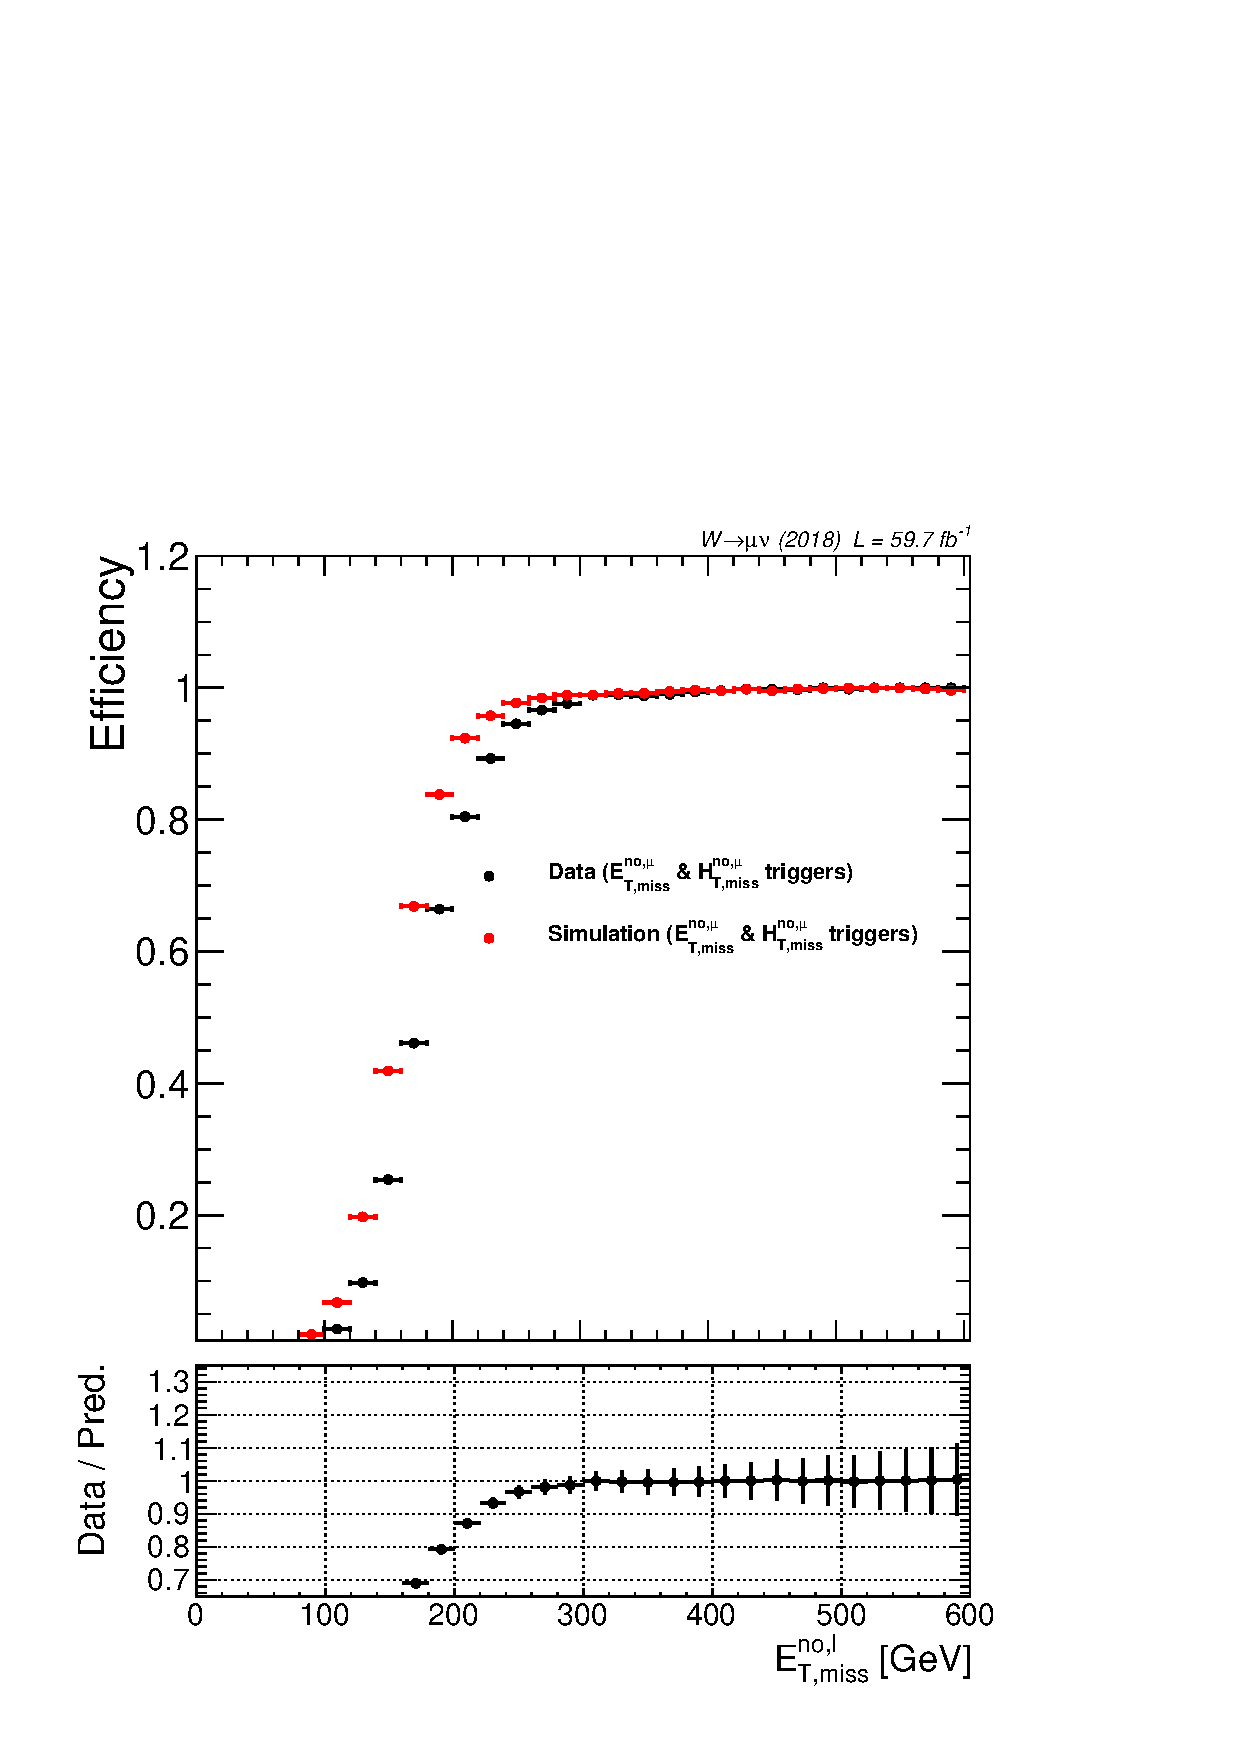
\includegraphics[width=0.45\textwidth]{Analysis_strategy/METMHT_eff/MetNoMuMETMHT_2018.pdf}
    }
  \caption{Trigger efficiencies for the MTR forming algorithms presented in $E_{T.miss}^{no,\mu}$ bins for both eras. Separate efficiencies were measured for data and simulation with the resulting scale factor also being shown.}
  \label{fig:metmht_effs}
\end{figure}


\hspace{10pt} An additional set of efficiencies was produced by separating jets into three categories by looking at the geometrical properties of the two leading jets. This has resulted into three categories: two central jets (CC), one central, one forward jet (CF) and two forward jets (FF). This study was prompted as safety check in order to confirm that a previously reported dip in $m_{jj}$ efficiency during the 2016 era~\cite{note:AN_16_418} has disappeared after mitigation. The origin of this efficiency loss was the exclusion of the HF region from the energy sums at the L1T level. Summary of this study is that the lack of efficiency issues plaguing the previous era has been correctly removed through the addition of the HF contribution implemented for the 2017 and 2018 eras. Figure~\ref{fig:metmht_test} summarises these results by presenting the efficiencies in both the $E_{T,miss}^{~no,\mu}$ and $m_{jj}$ bins. The added $E_{T,miss}^{~no,\mu}$ option was included in order to have a confirmation that no significant deviations appear between two higher statistics regions (CC and CF).


\begin{figure}[htbp]
  \centering
    \subfigure[$E_T^{miss}$ - 2017 (data)]{
    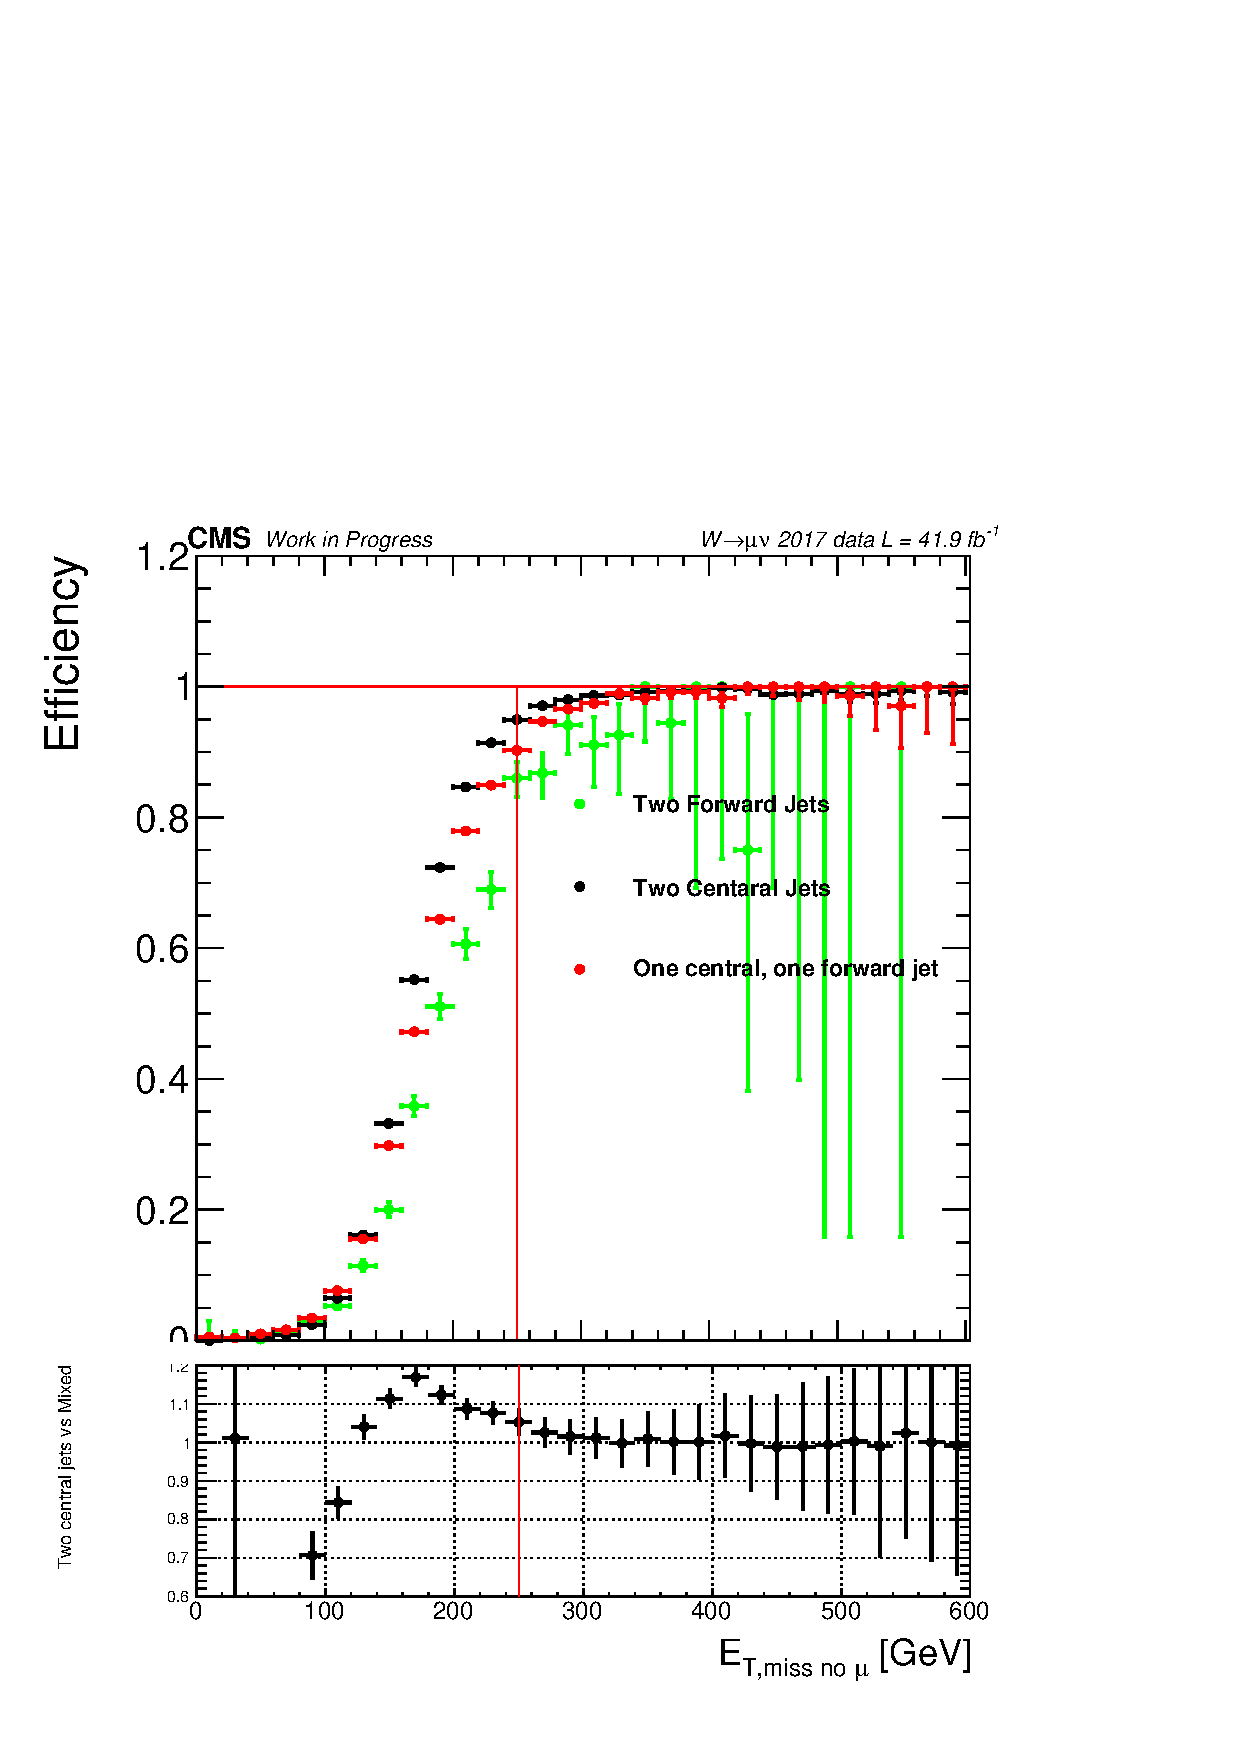
\includegraphics[width=0.45\textwidth]{Analysis_strategy/METMHT_eff/MetNoMuMETMHT_2017data_case_study.pdf}
    }
    \subfigure[$E_T^{miss}$ - 2017 (simulation)]{
    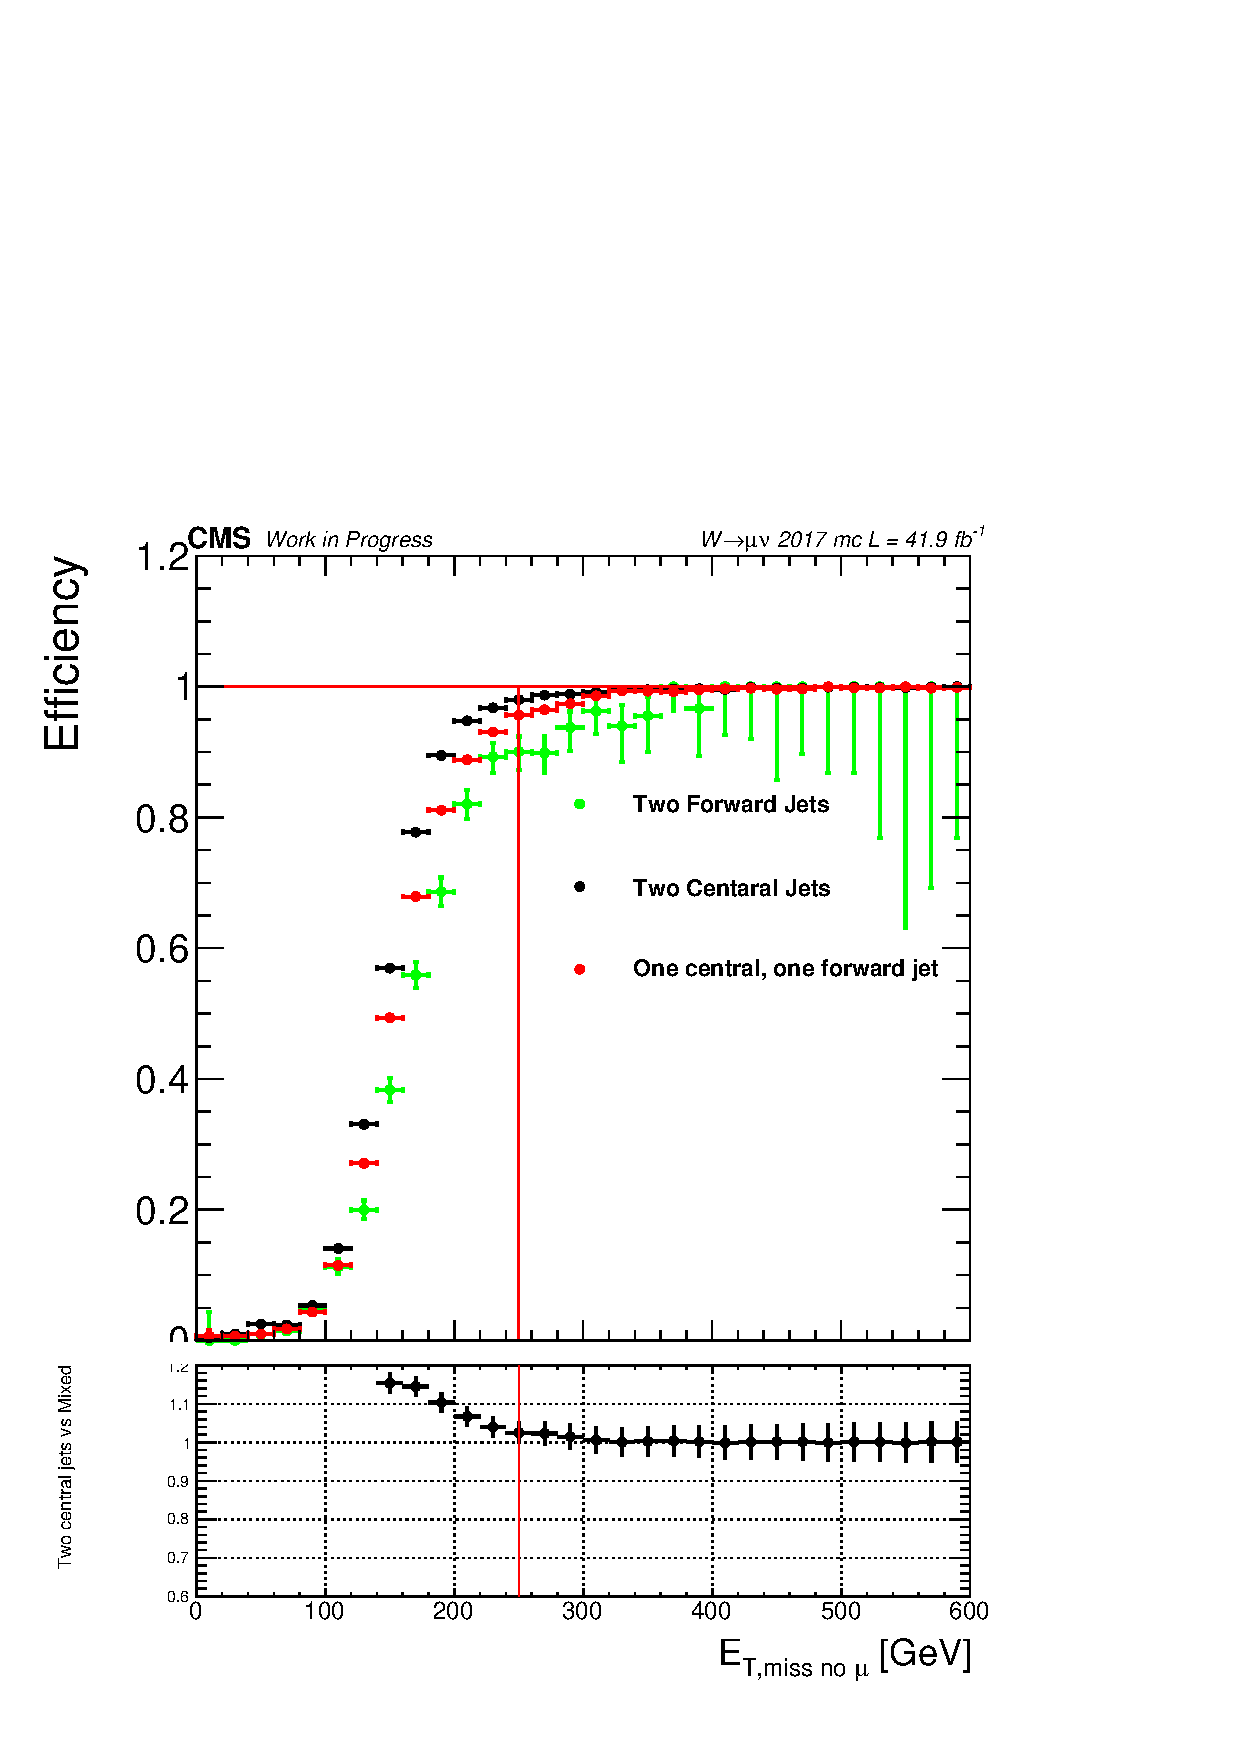
\includegraphics[width=0.45\textwidth]{Analysis_strategy/METMHT_eff/MetNoMuMETMHT_2017mc_case_study.pdf}
    }\\
    \subfigure[$E_T^{miss}$ -  2018 (data)]{
    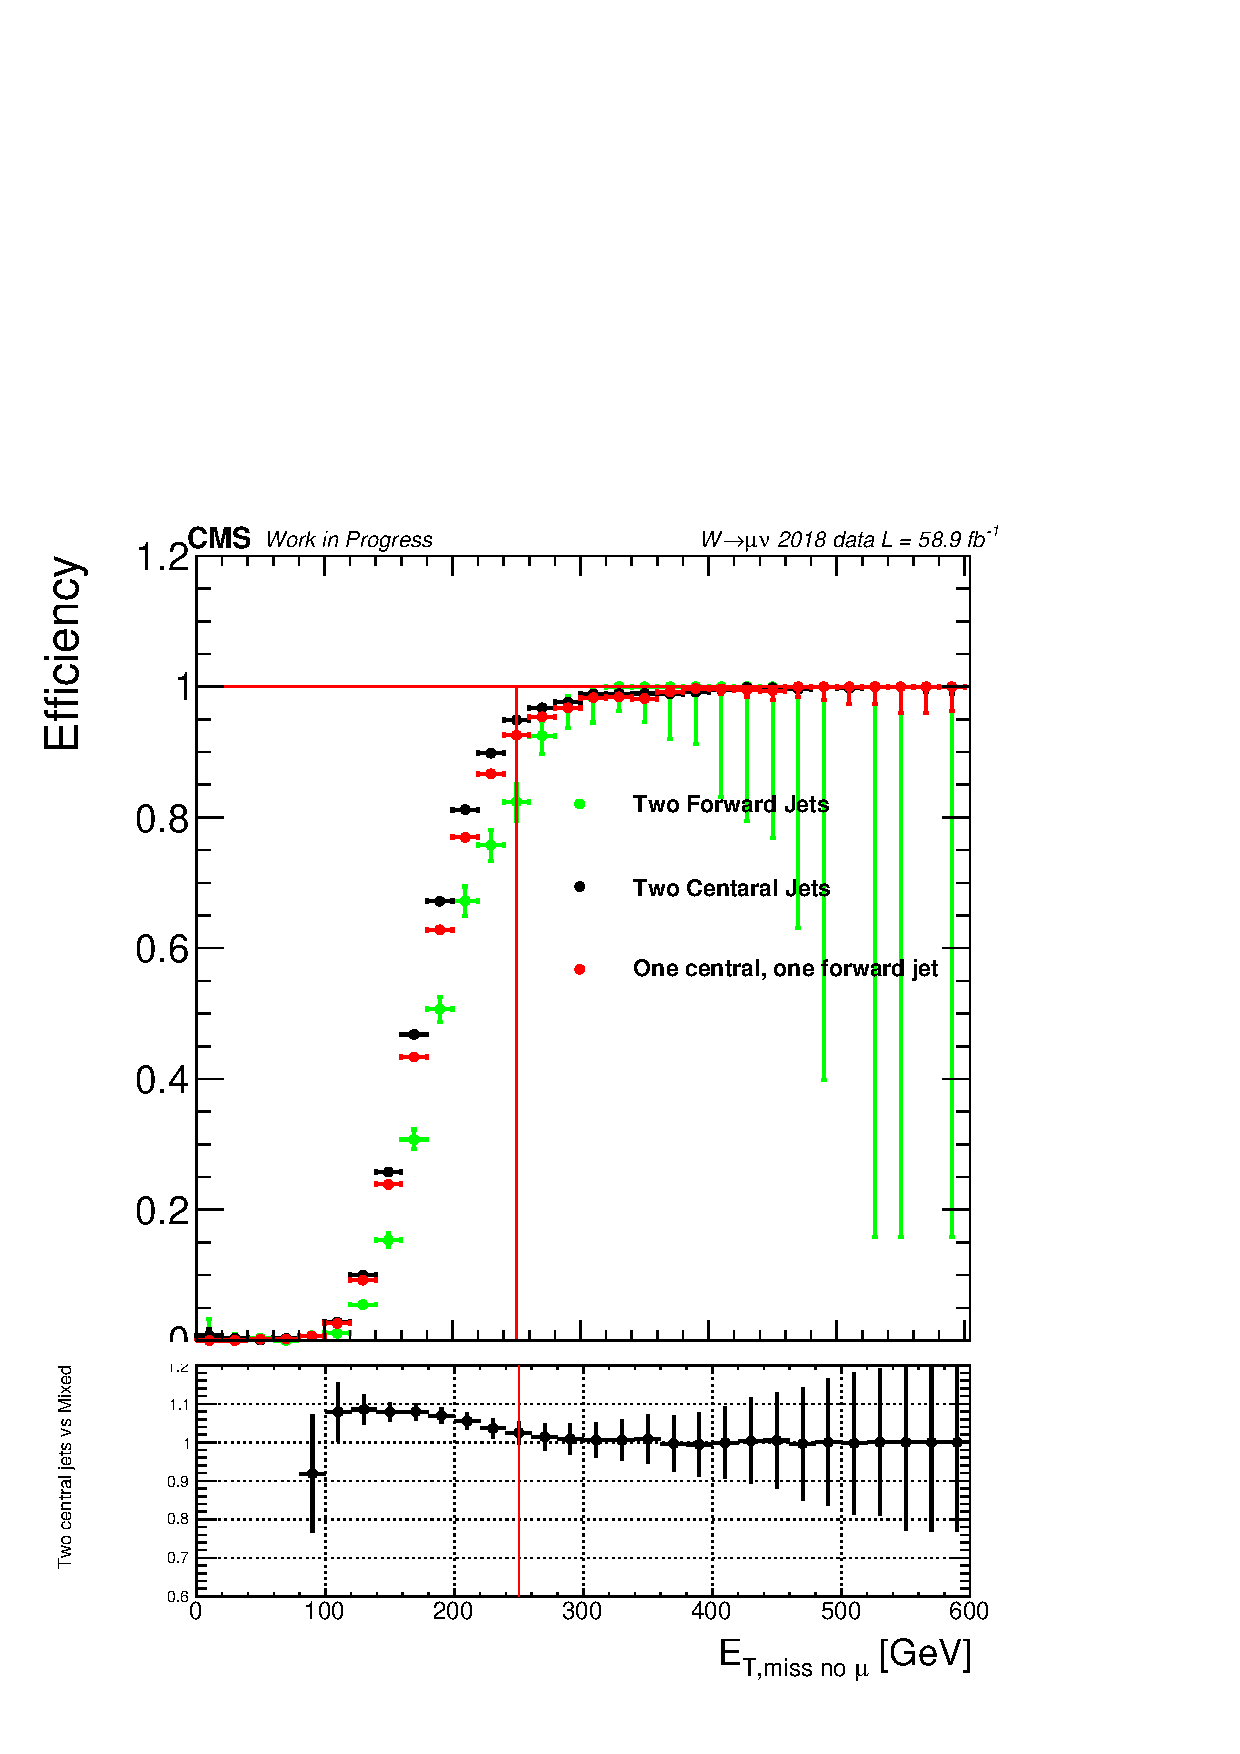
\includegraphics[width=0.45\textwidth]{Analysis_strategy/METMHT_eff/MetNoMuMETMHT_2018data_case_study.pdf}
    }
    \subfigure[$E_T^{miss}$ -  2018 (simulation)]{
    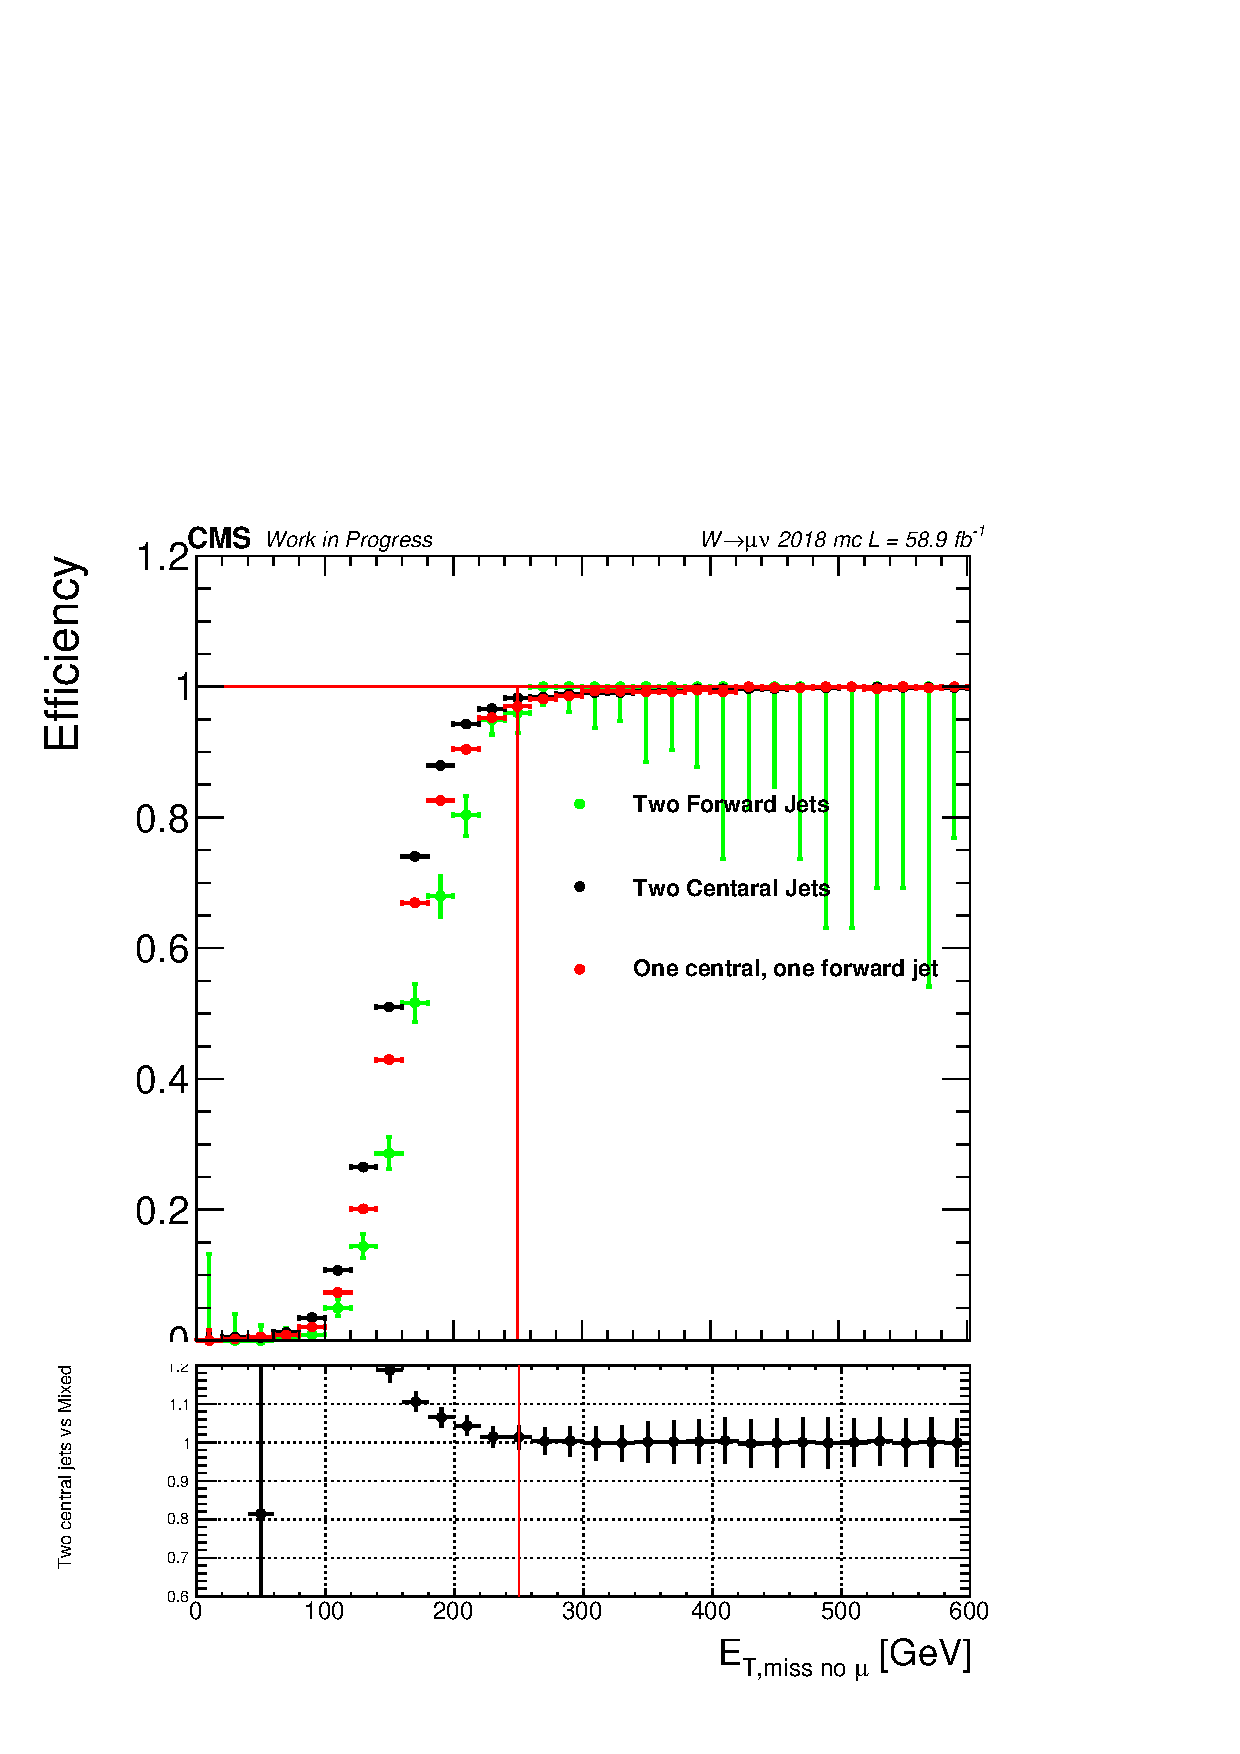
\includegraphics[width=0.45\textwidth]{Analysis_strategy/METMHT_eff/MetNoMuMETMHT_2018mc_case_study.pdf}
    }
  \caption{Trigger efficiencies for the MTR forming algorithms presented in $E_{T.miss}^{no,\mu}$ bins for both eras (computed for data and simulation). Separation into three different jet $\eta$ regions (CC, CF and FF) is performed. The resulting comparison between the CC and CF is also presented with the ratio plot. }
  \label{fig:metmht_test}
\end{figure}


\begin{figure}[htbp]
  \centering
    \subfigure[$m_{jj}$ - 2017 (data)]{
    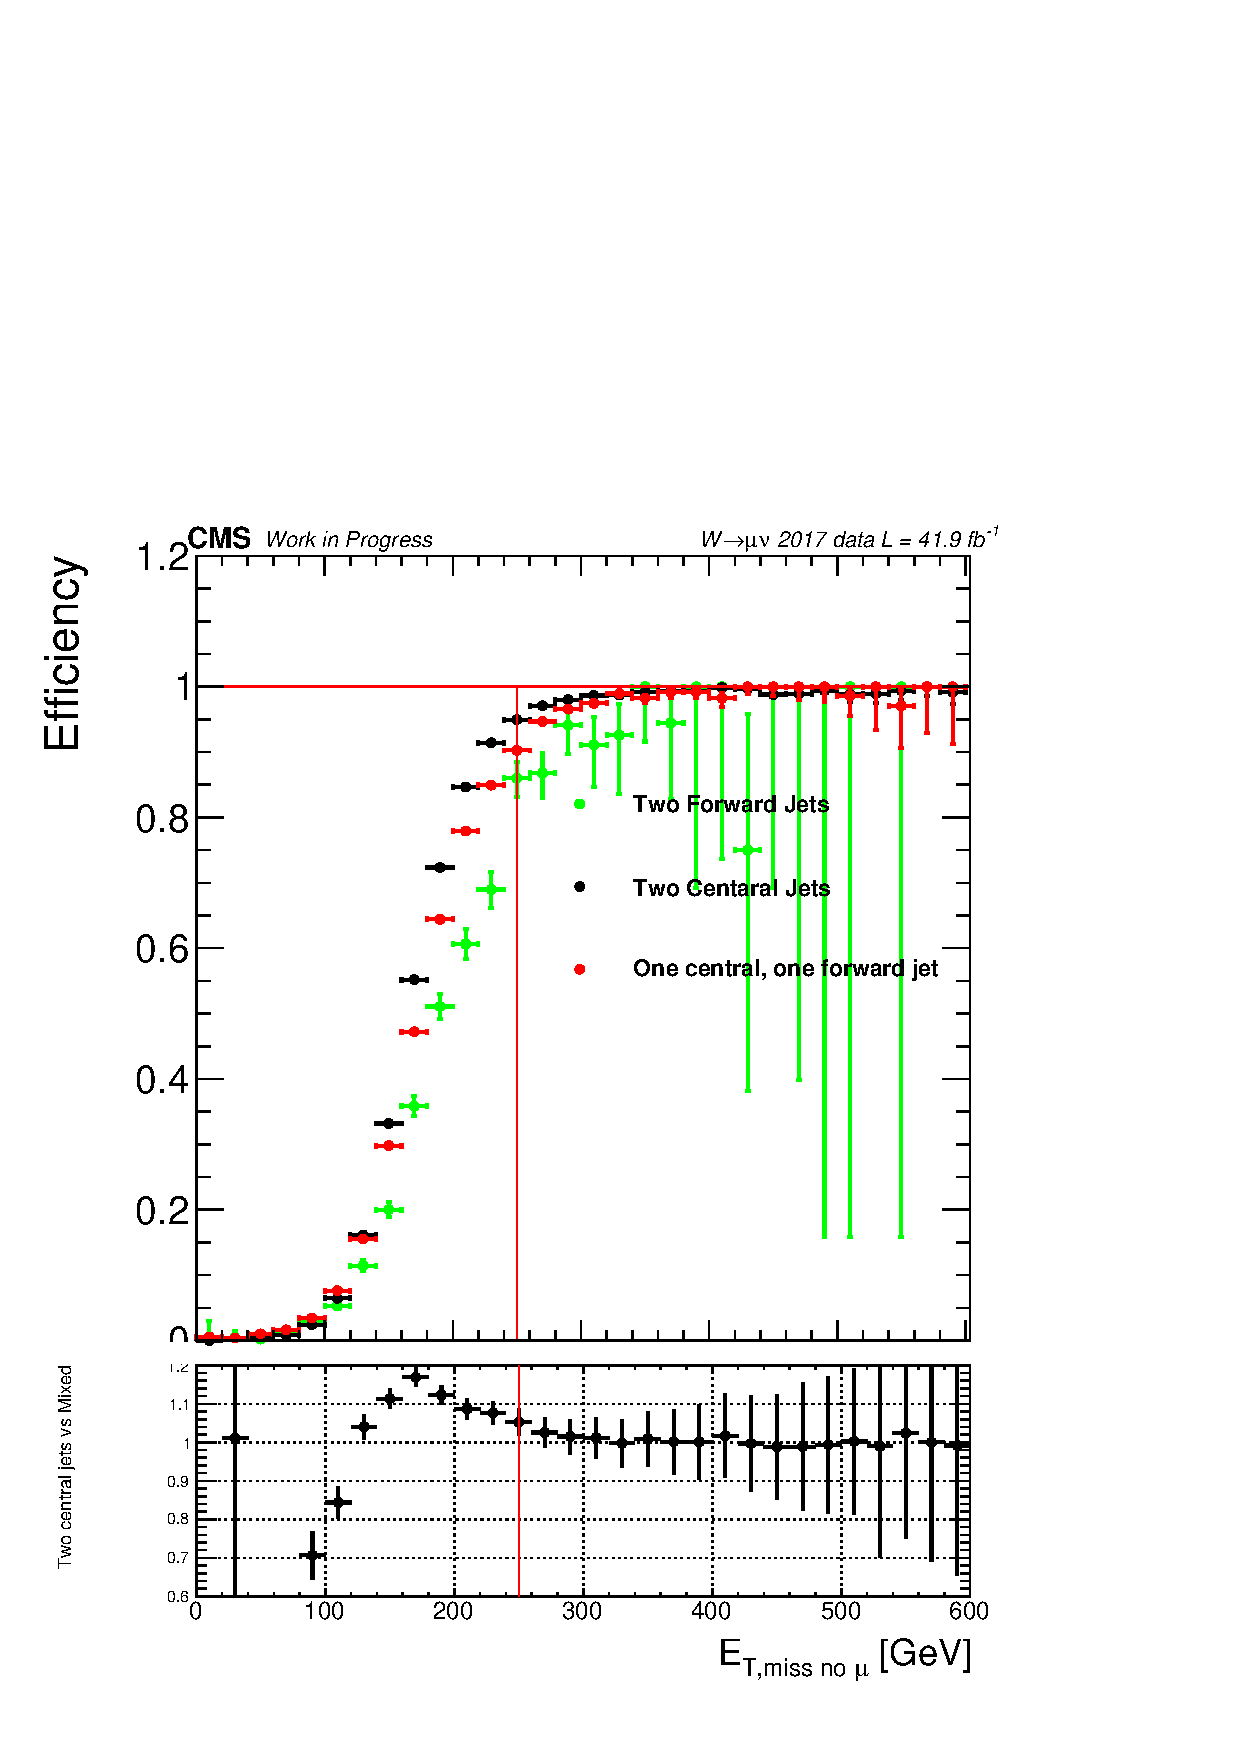
\includegraphics[width=0.45\textwidth]{Analysis_strategy/METMHT_eff/MetNoMuMETMHT_2017data_case_study.pdf}
    }
    \subfigure[$m_{jj}$ - 2017 (simulation)]{
    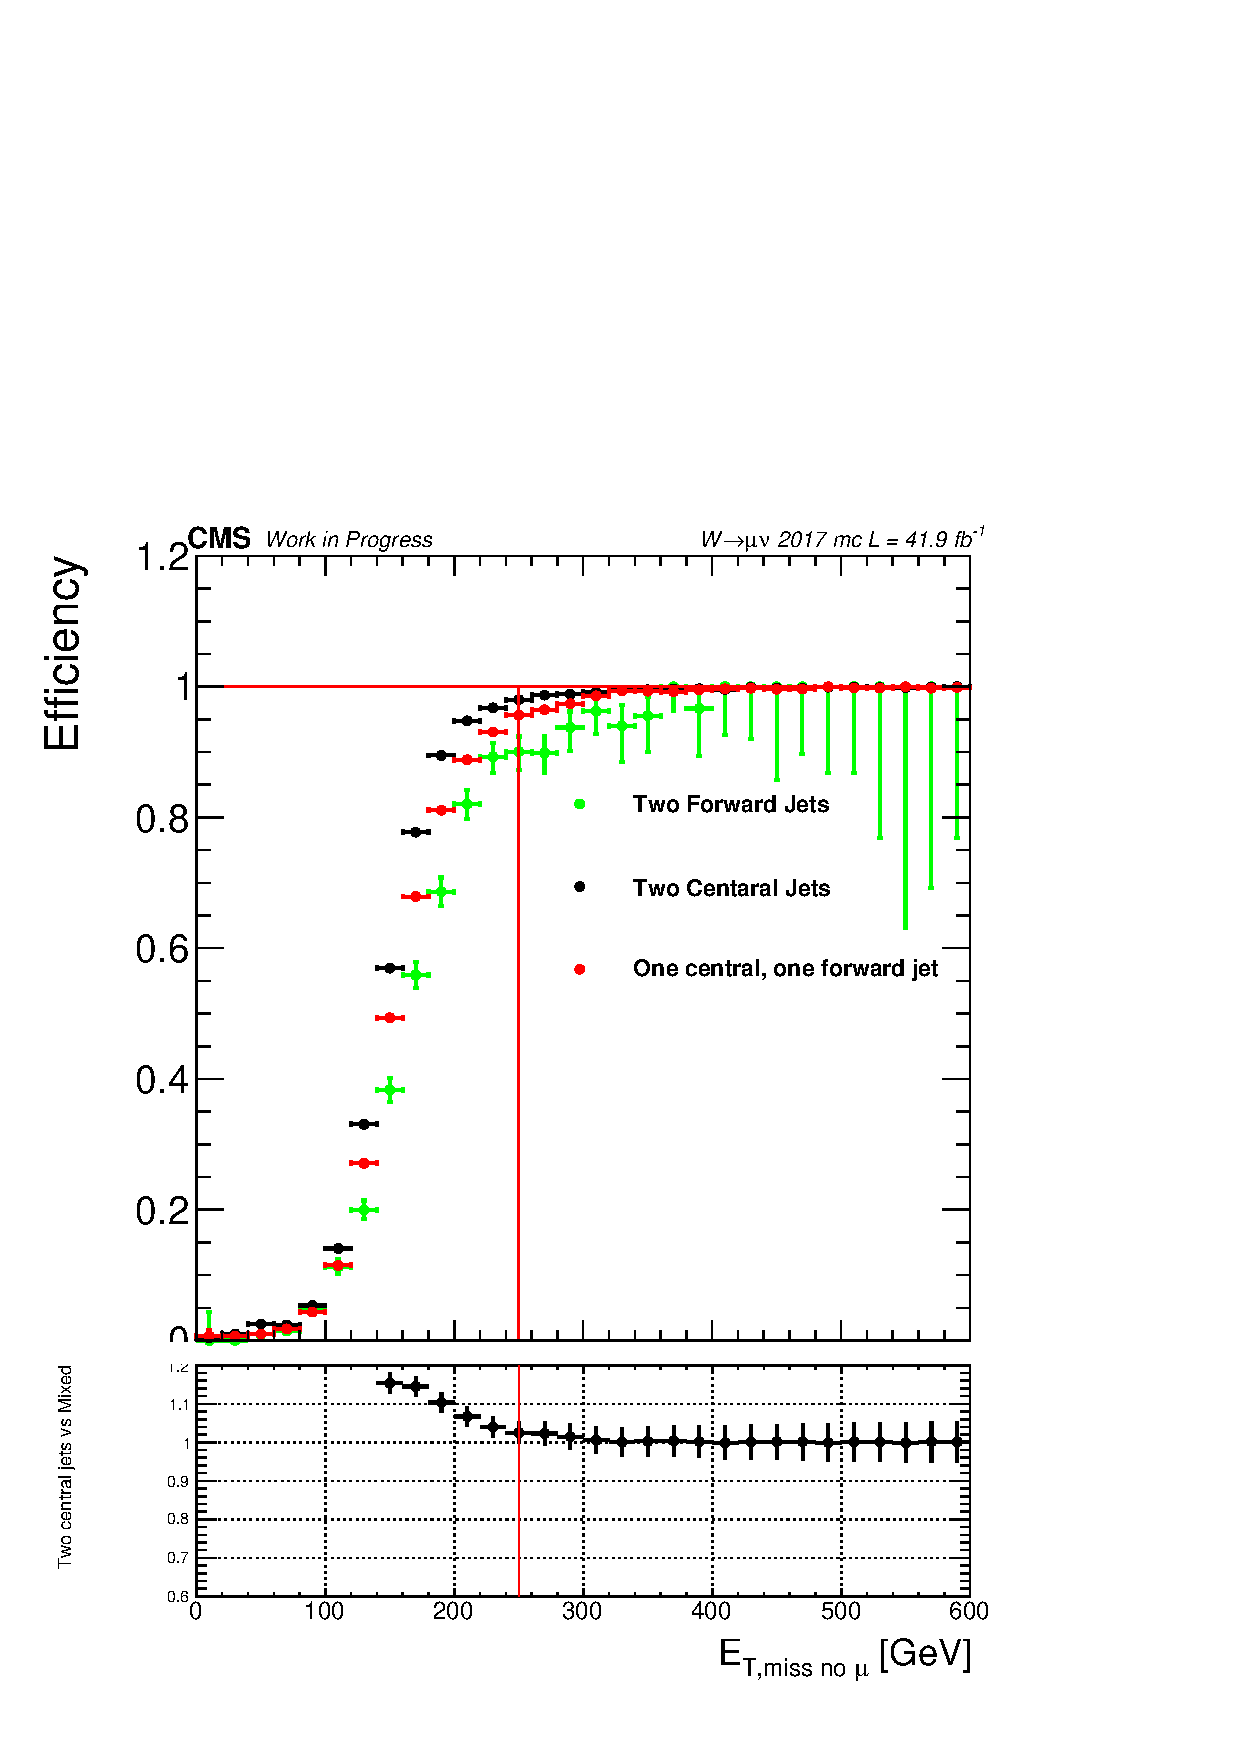
\includegraphics[width=0.45\textwidth]{Analysis_strategy/METMHT_eff/MetNoMuMETMHT_2017mc_case_study.pdf}
    }\\
    \subfigure[$m_{jj}$ - 2018 (data)]{
    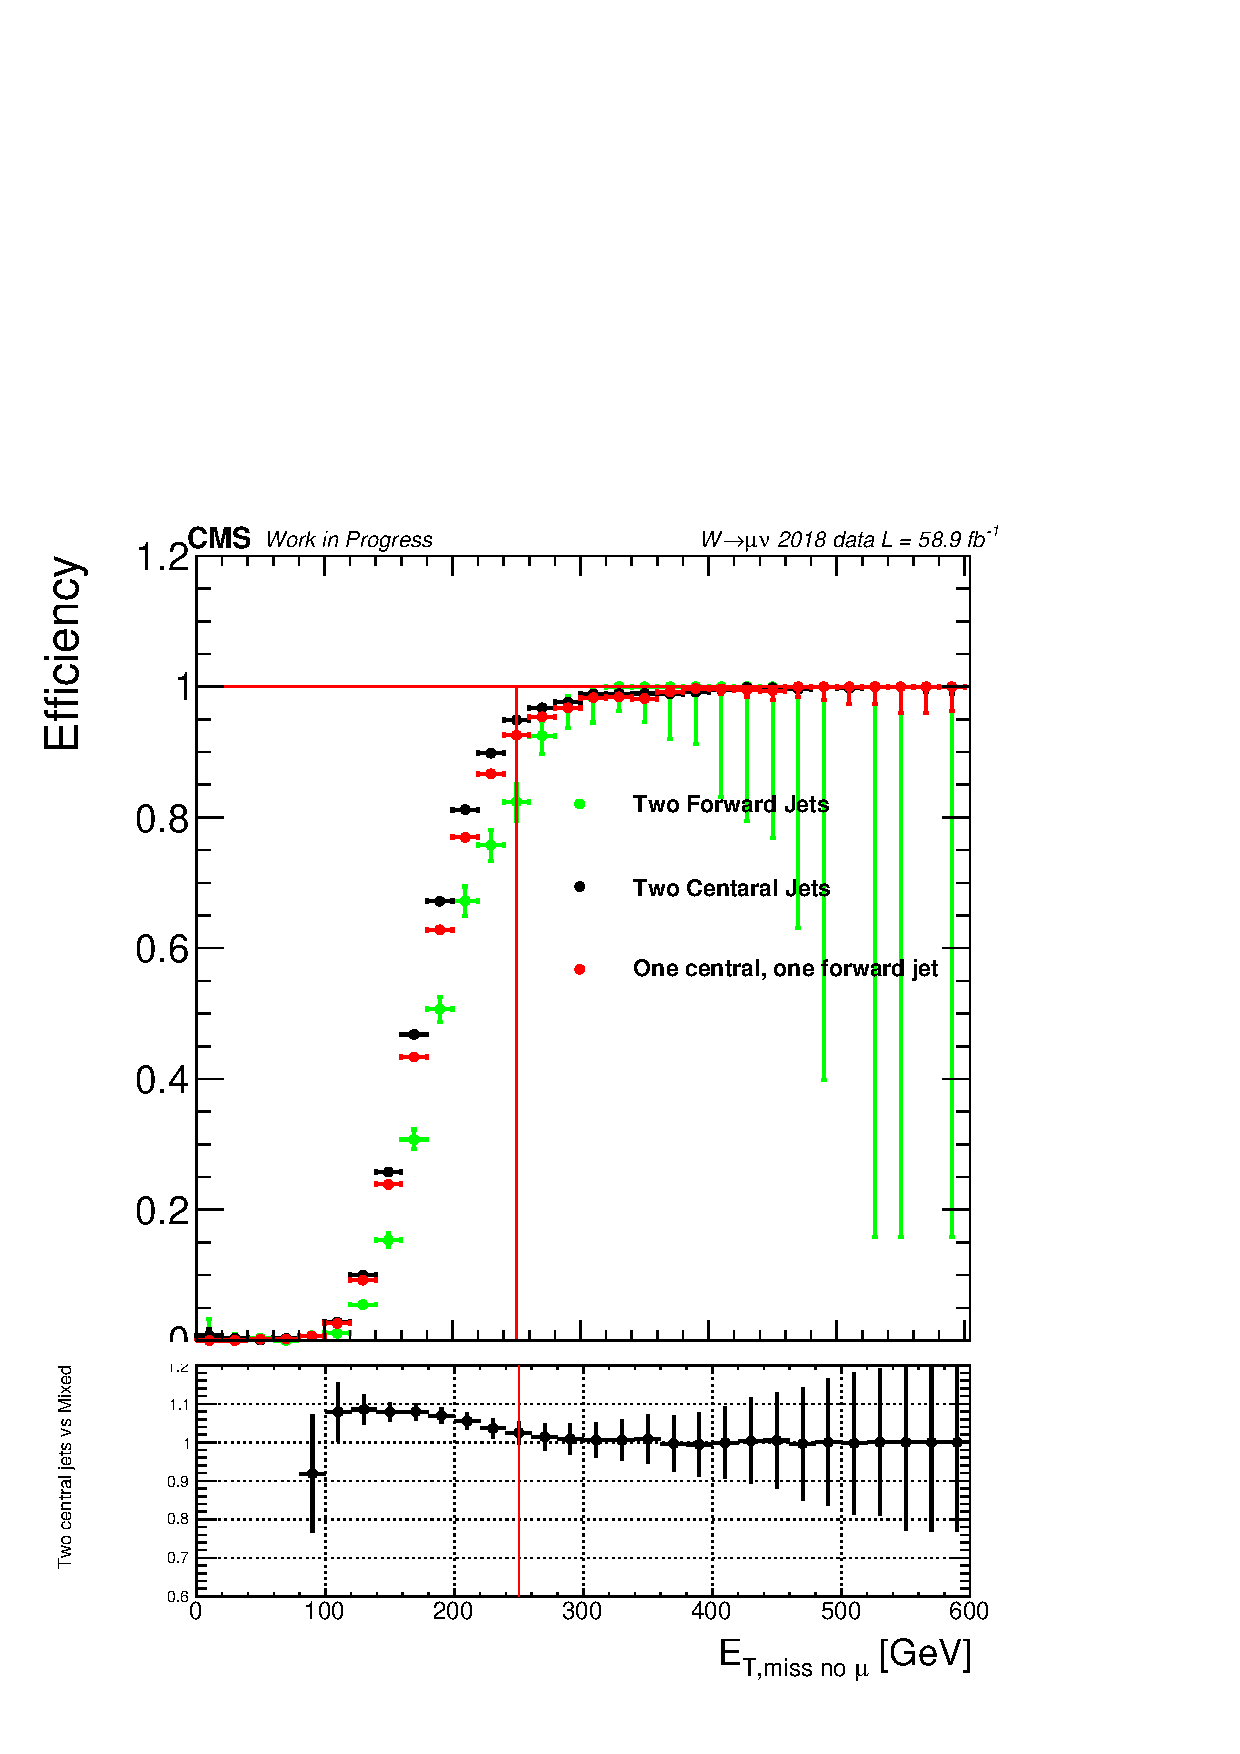
\includegraphics[width=0.45\textwidth]{Analysis_strategy/METMHT_eff/MetNoMuMETMHT_2018data_case_study.pdf}
    }
    \subfigure[$m_{jj}$ - 2018 (simulation)]{
    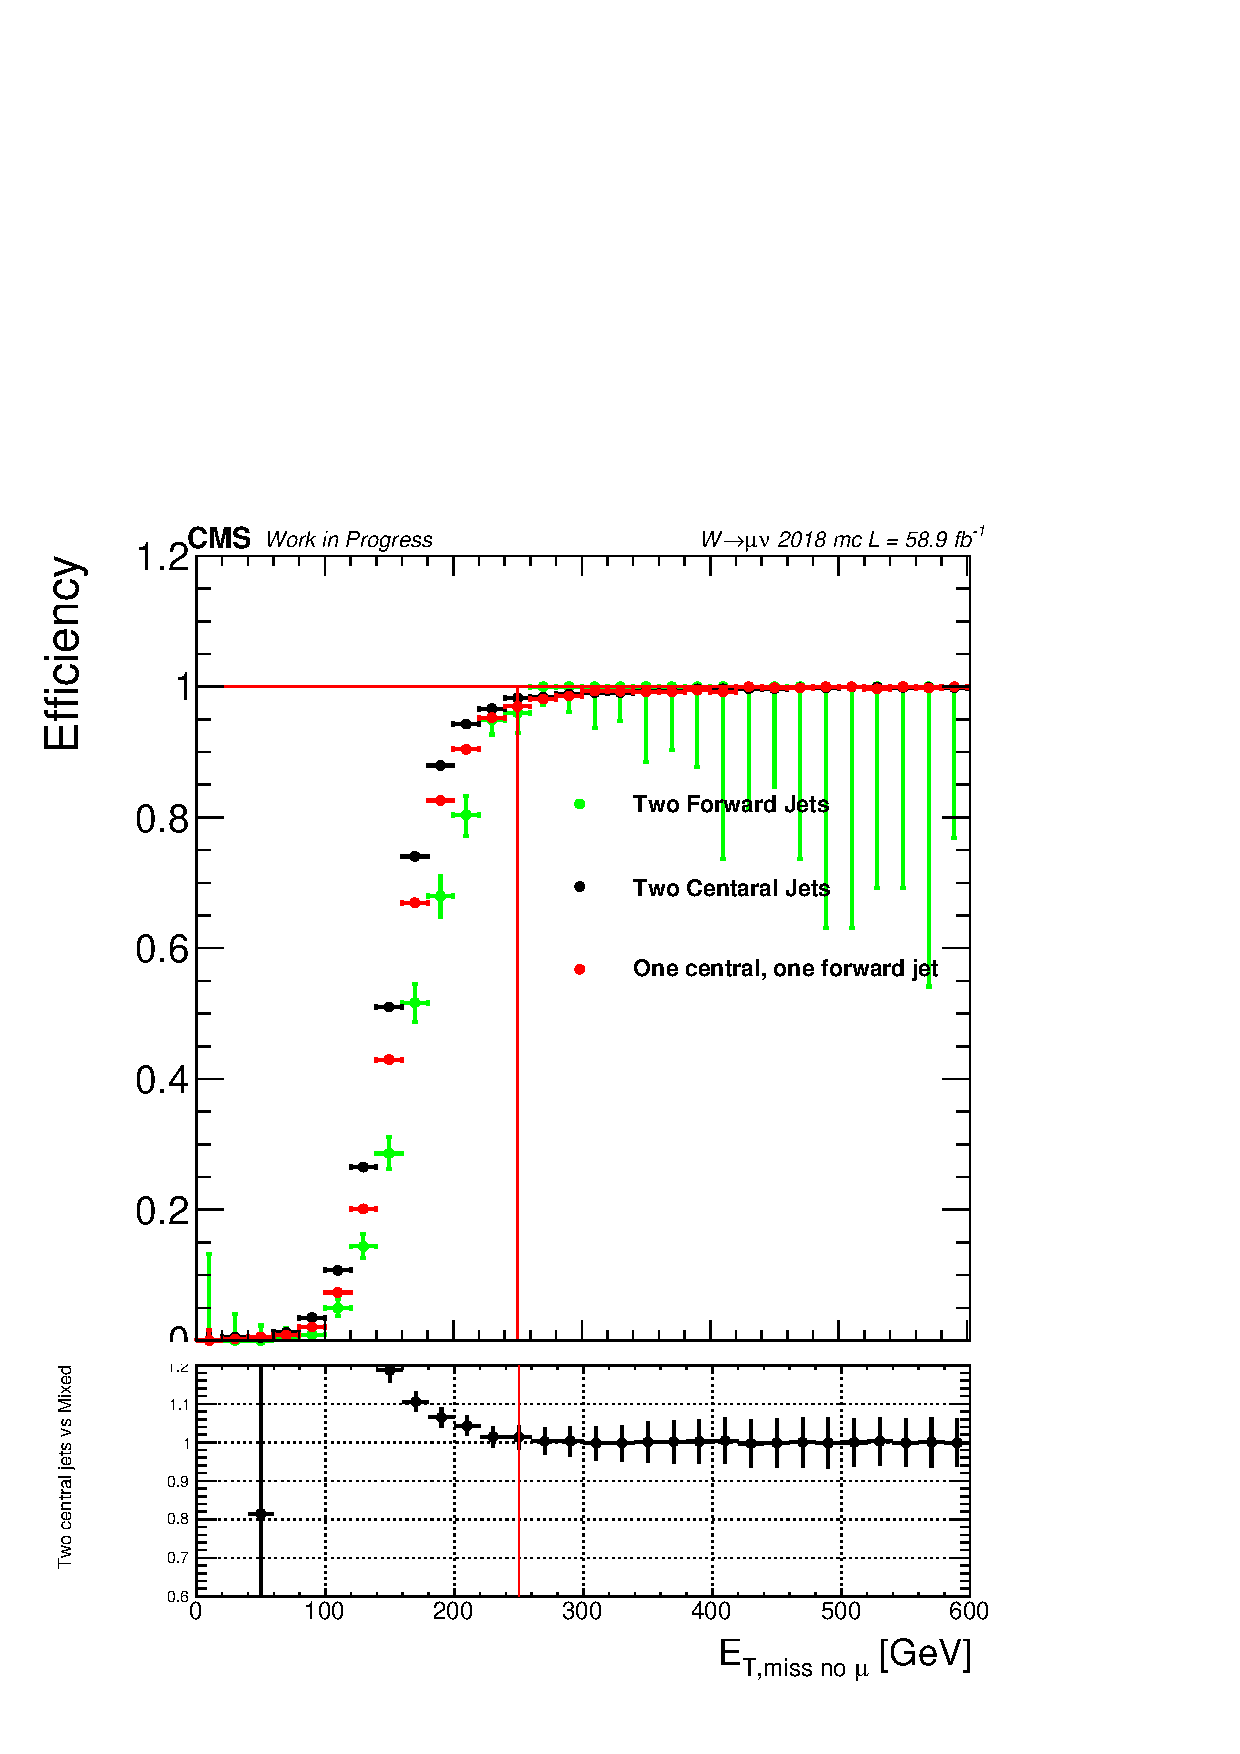
\includegraphics[width=0.45\textwidth]{Analysis_strategy/METMHT_eff/MetNoMuMETMHT_2018mc_case_study.pdf}
    }
  \caption{Trigger efficiencies for the MTR forming algorithms presented in $m_{jj}$ bins for both eras (computed for data and simulation). Separation into three different jet $\eta$ regions (CC, CF and FF) is performed. The resulting comparison between the CC and CF is also presented with the ratio plot.}
  \label{fig:metmht_test}
\end{figure}

%\hspace{10pt} In order to ensure that the variations between regions have been accounted for, a comparison of trigger efficiencies for the single and double muon regions is performed. The double muon region is formed in mostly the same way as the single muon region, with the difference being the request that there exist exactly two muons (at least one of which needs to pass the tight requirements) in the event. Conclusion on regarding this study.


%%%%%%%%%%%%%% END OF METMHT PART %%%%%%%%%%%%%%%%%%%%%%%%%%%%%%%%




\subsection{Performance of VBF triggers}
\label{sec:vbf_trigger_performance}

\hspace{10pt} Similarly to previously described efficiency study regarding the MTR forming triggers, the first step when approaching the VBF triggers is the formation of the single muon region. From this point, the general approach takes a slightly different turn. As the MTR category relied on already proven, optimised selection, the VBF triggers brought a new part of the phase space that is yet to be explored. Staring from the information about the building blocks of VBF paths (discussed in Section~\ref{sec:vbf_trgger}), the next step was the optimisation the of the selection requirements for three main variables: $m_{jj}$, $p_{T,j1}$ and $p_{T,j2}$. In order to follow the trigger logic, the selection of the dijet pair is going be based around the largest $m_{jj}$ logic.

\hspace{10pt} Figure~\ref{fig:vbf_trig_mjj_opt} shows the resulting efficiency of the logical OR of both VBF triggers presented in terms of $m_{jj}$ bins, where the thresholds for the other two main variables are being kept high enough to ensure that an unbiased decision can be made. The resulting requirement of $m_{jj}>$~900~GeV is motivated by the desire to stay above the $95$~\% trigger efficiency in data. Figure~\ref{fig:vbf_trig_pt_opt} presents results of equivalent optimisation studies performed for the purposes of tailoring selection requirements for the jet $p_T$ variables.

\begin{figure}[htbp]
  \centering
    \subfigure{
    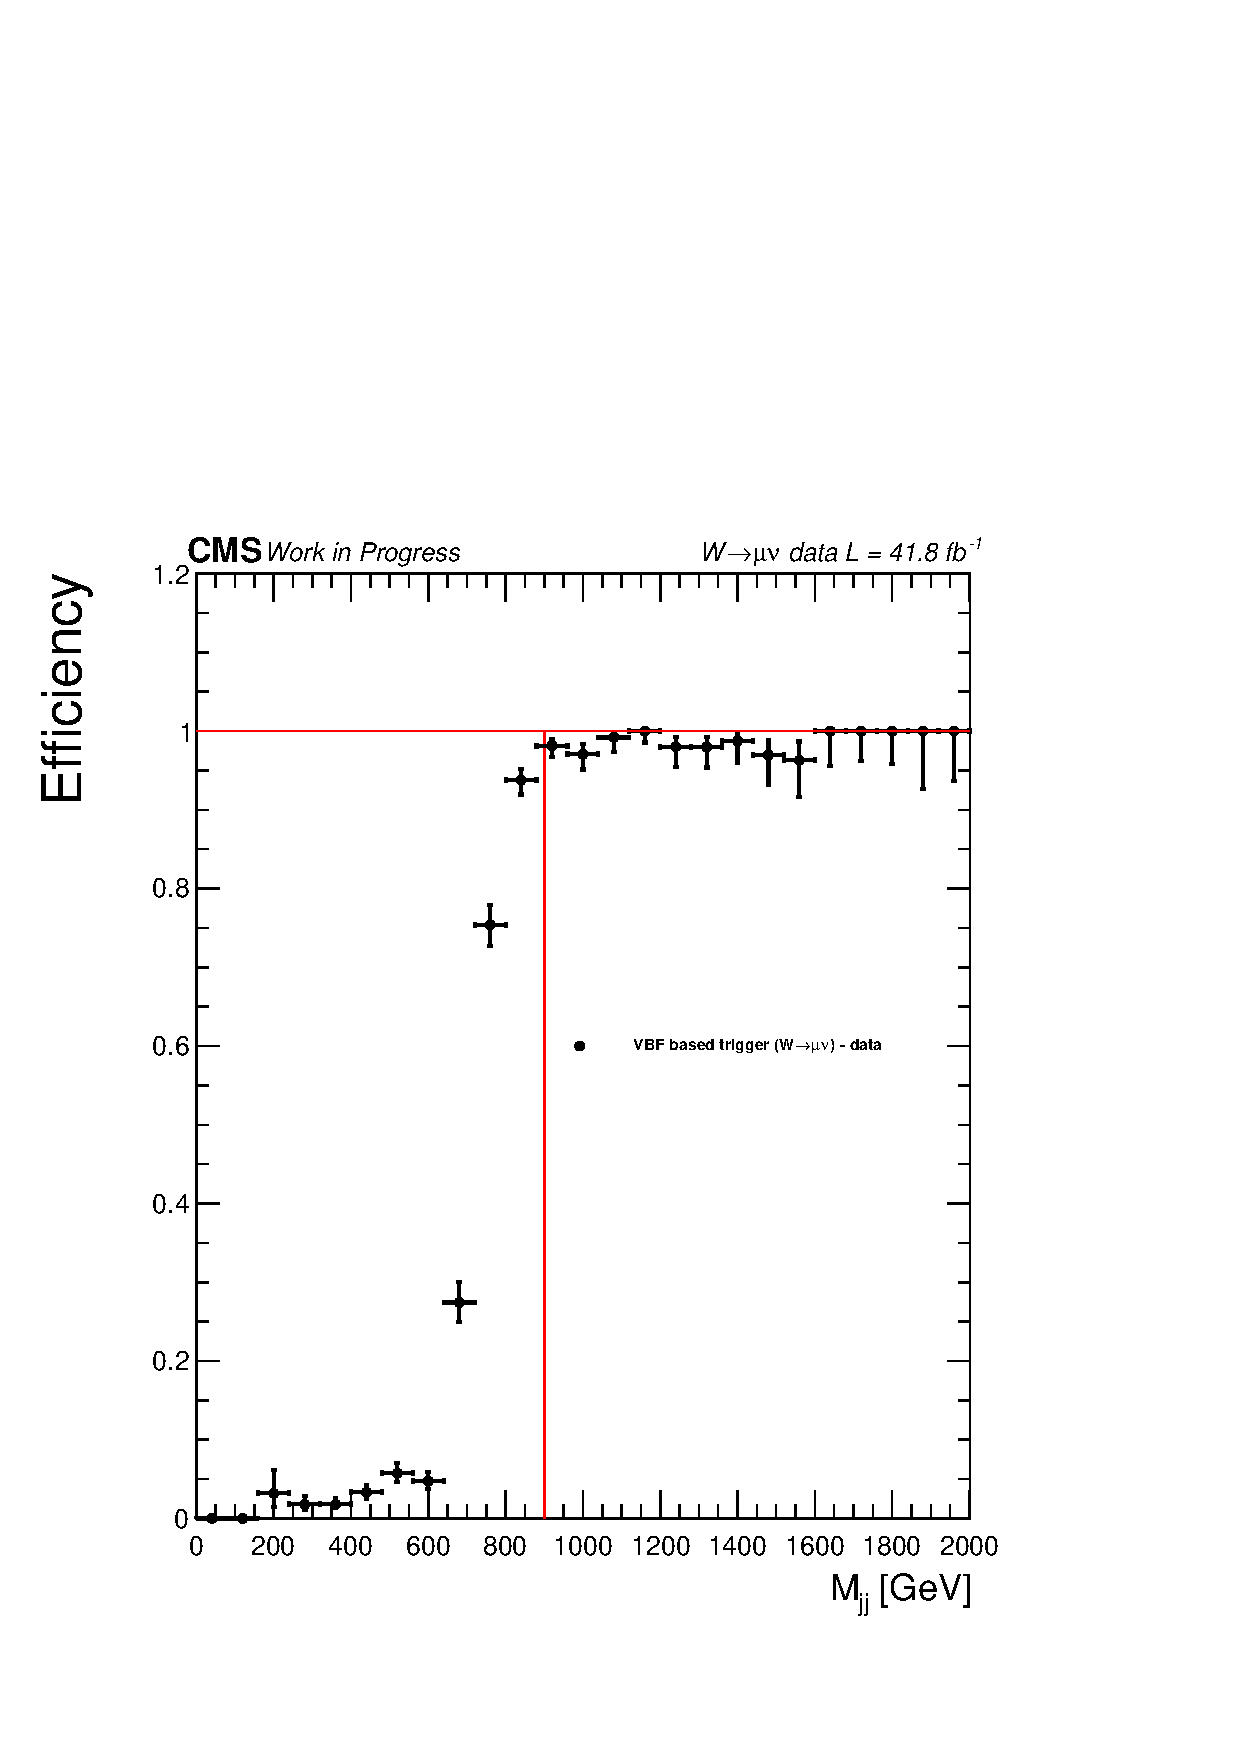
\includegraphics[width=0.45\textwidth]{Analysis_strategy/VBF_eff/2017/lMjjVBF_1.pdf}
    }
\caption{Trigger efficiency of the logical OR of both VBF triggers (performed in data), presented in $m_{jj}$ bins used to motivate a selection requirement for this variable.}
\label{fig:vbf_trig_mjj_opt}
\end{figure}

\begin{figure}[htbp]
  \centering

    \subfigure[$p_{T,j1}$ efficiency]{
    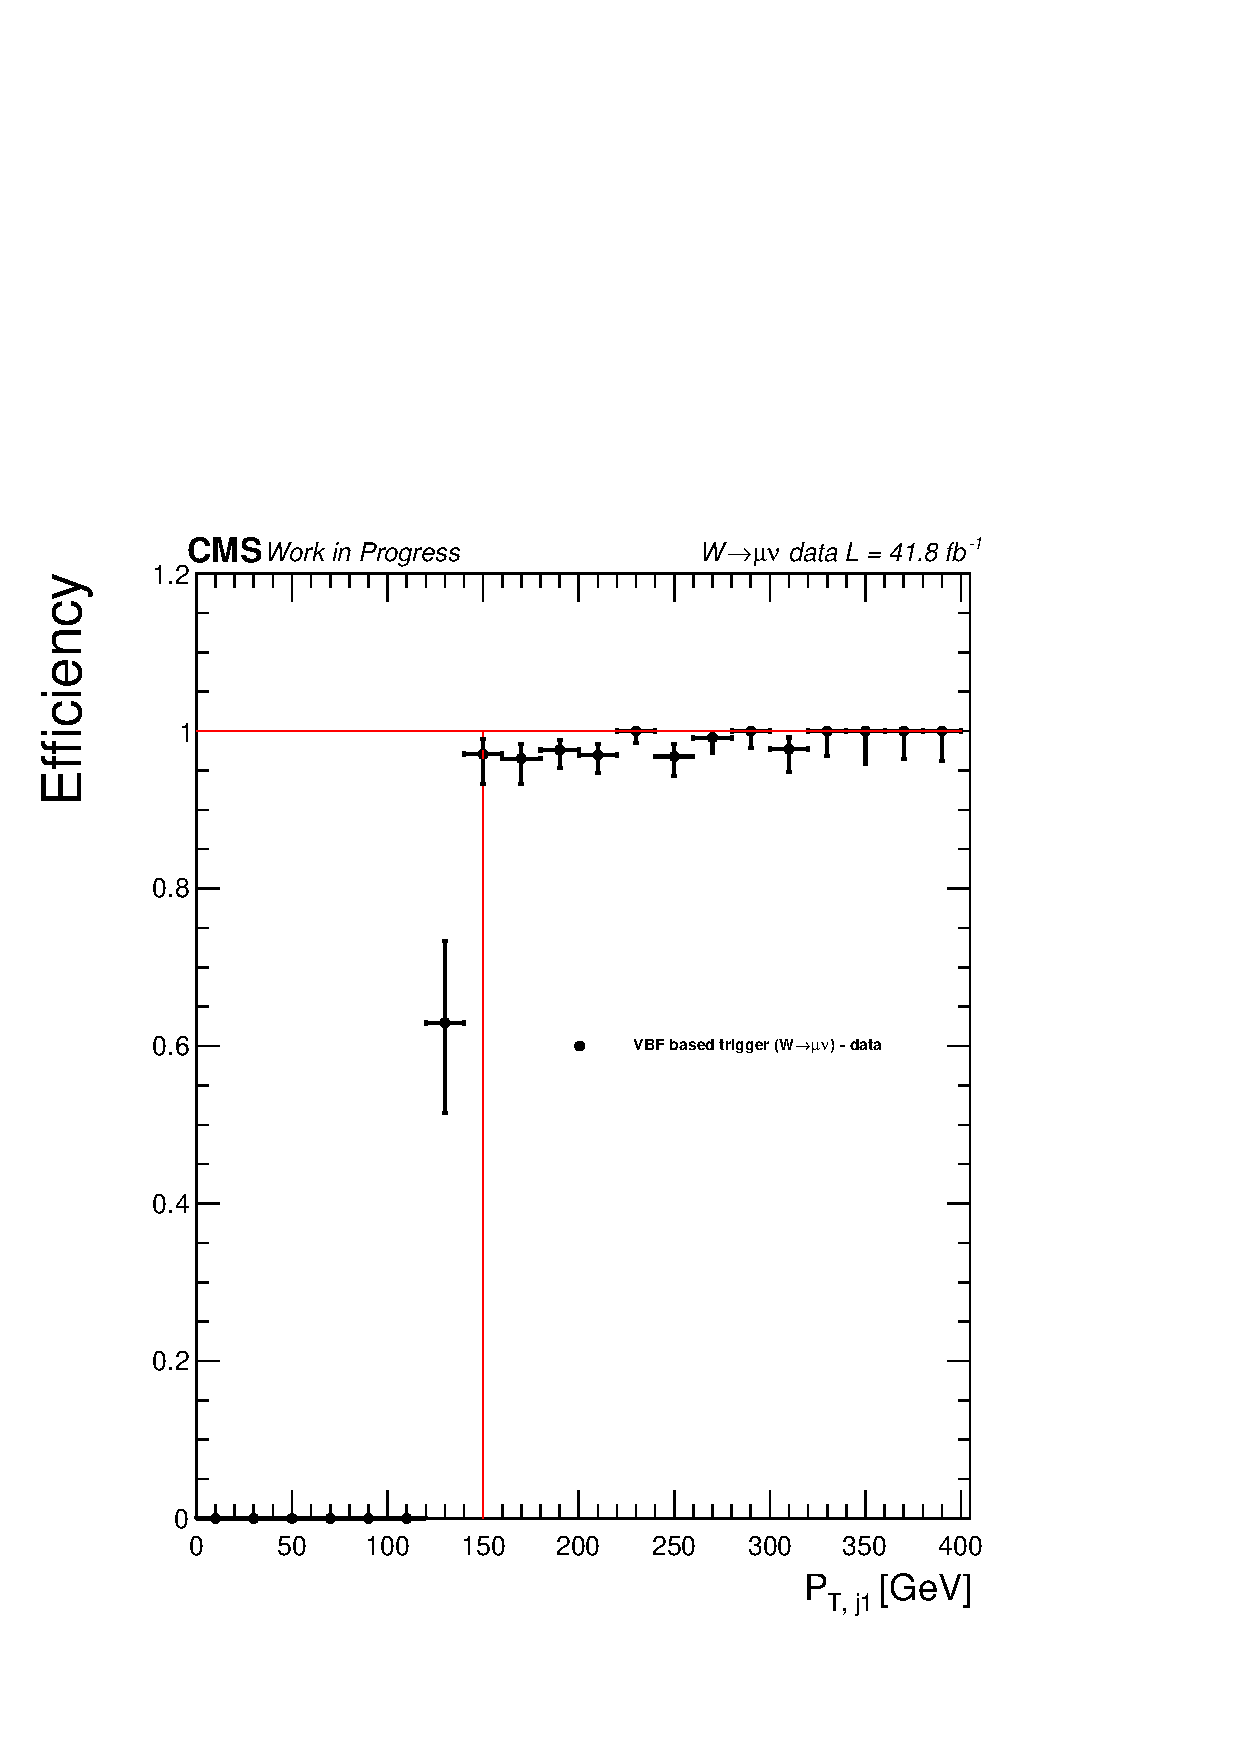
\includegraphics[width=0.45\textwidth]{Analysis_strategy/VBF_eff/2017/lMjj_jet1_ptVBF_1.pdf}
    }
    \subfigure[$p_{T,j2}$ efficiency]{
    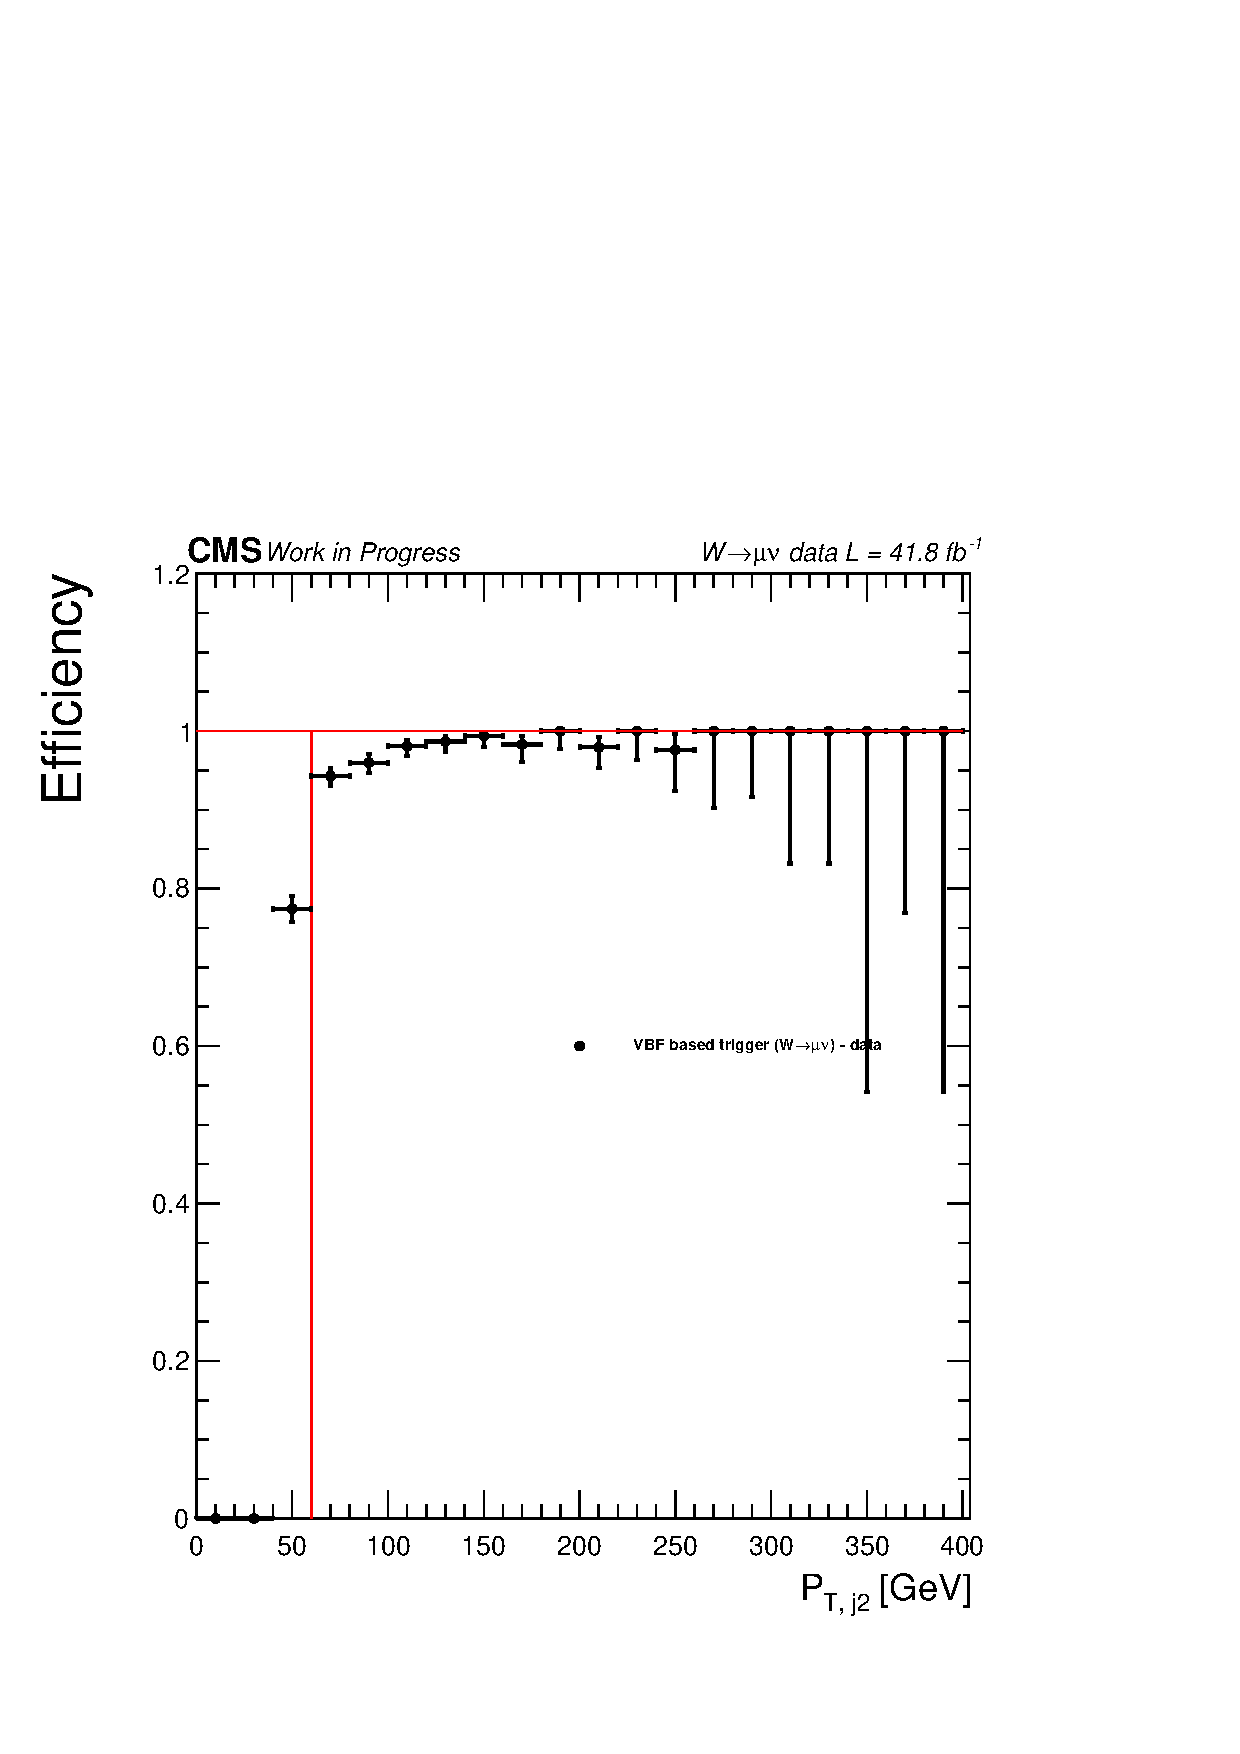
\includegraphics[width=0.45\textwidth]{Analysis_strategy/VBF_eff/2017/lMjj_jet2_ptVBF_1.pdf}
    }
  \caption{Trigger efficiency of the logical OR of both VBF triggers (performed in data), presented in $p_T$ bins for the leading (left) and subleading (right) jet, used to motivate selection requirements for these variable.}
  \label{fig:vbf_trig_pt_opt}
\end{figure}

\hspace{10pt} Following the high thresholds on jet properties, the difference between selecting the two leading $p_T$ jets and the ones forming the largest $m_{jj}$ is small enough that it brings the option of using the rest of the already optimised MTR requirements into the VTR selection. At this stage, these requirements form almost the final VTR category, differing only with the $min\Delta\phi(j, E_{T,miss})>$0.5 requirement. Figure~\ref{fig:vbf_proto_trig_eff} shows the data to simulation comparison of the performance of VBF triggers for both eras (for the current, proto-VTR, selection requirements).

\begin{figure}[htbp]
  \centering
    \subfigure[$E_{T,miss}$ - 2017]{
    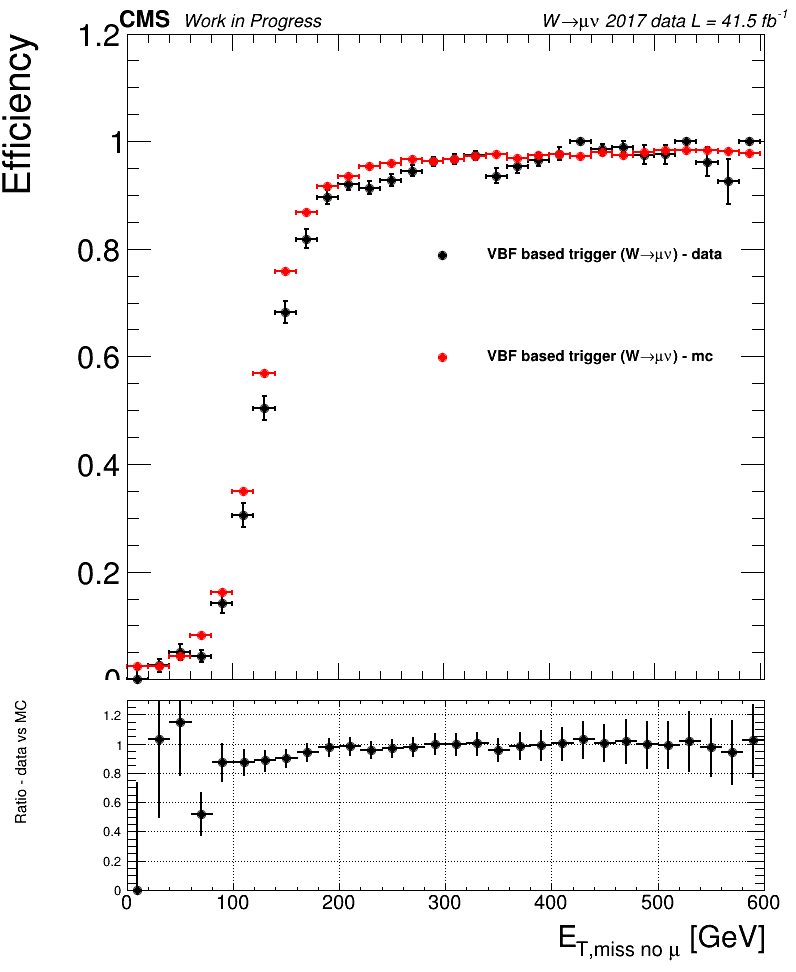
\includegraphics[width=0.45\textwidth]{Analysis_strategy/VBF_eff/VBF_trig_2017_proto.png}
    }
    \subfigure[$E_{T,miss}$ - 2018]{
    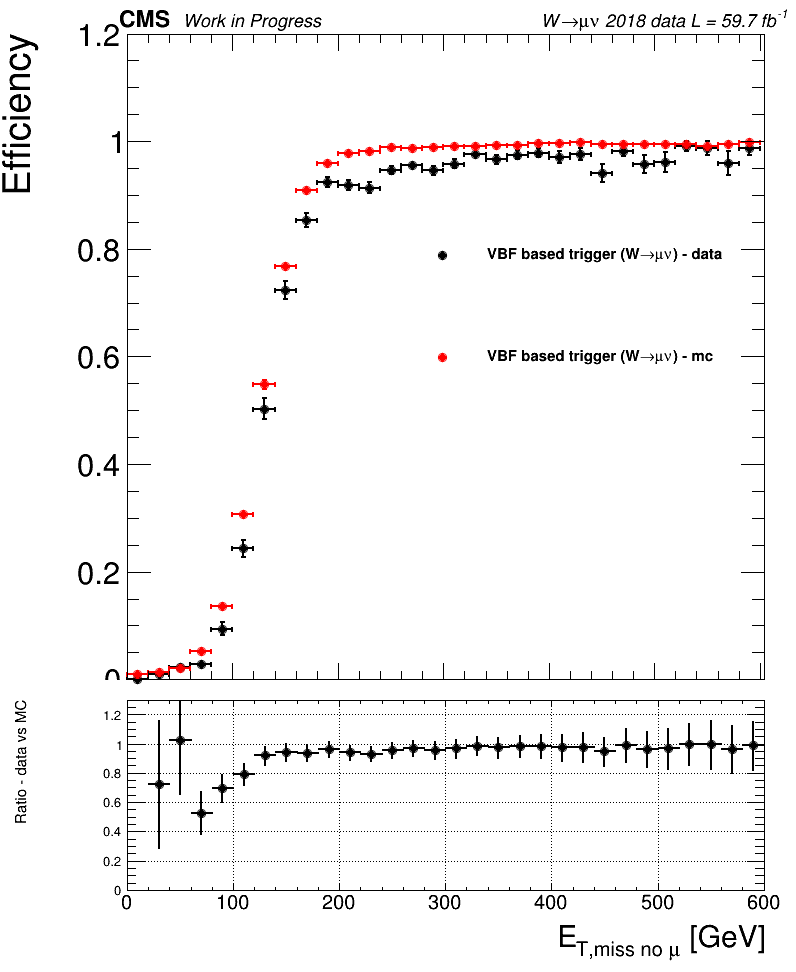
\includegraphics[width=0.45\textwidth]{Analysis_strategy/VBF_eff/VBF_trig_2018_proto.png}
    }
  \caption{Trigger efficiency of the logical OR of both VBF triggers, presented in $E_{T,miss}$ measured using the proto-VTR selection requirements.}
  \label{fig:vbf_proto_trig_eff}
\end{figure}

\hspace{10pt} The next step is the decision on the exact $E_{T,miss}$ range used to define the VTR category. In order to have a better overview, a comparison of performances for both sets of triggers needed to be compared. Figure~\ref{fig:vbf_metmht_comp} presents the comparison between two trigger groups. Better performance of VBF triggers in the lower $E_{T,miss}^{~no, \mu}$ range has motivated the choice of the range for VTR to be [160, 250)~GeV. The overlaying shape of the VBF H$\rightarrow$inv simulation sample is placed to illustrate the potential signal gain achieved by this choice.

\hspace{10pt} Upon forming the preliminary VTR selection and observing the background composition given with Figure~\ref{fig:VTR_mindphi}, a tighter selection requirement was imposed on the $min\Delta\phi(j, E_{T,miss})$ variable in order to battle the contribution originating from QCD multijet processes. Data to simulation efficiency comparison accompanied with the final scale factors used in the analysis are given in Figure~\ref{fig:vbf_trig_eff_final}.

\begin{figure}[htbp]
  \centering
    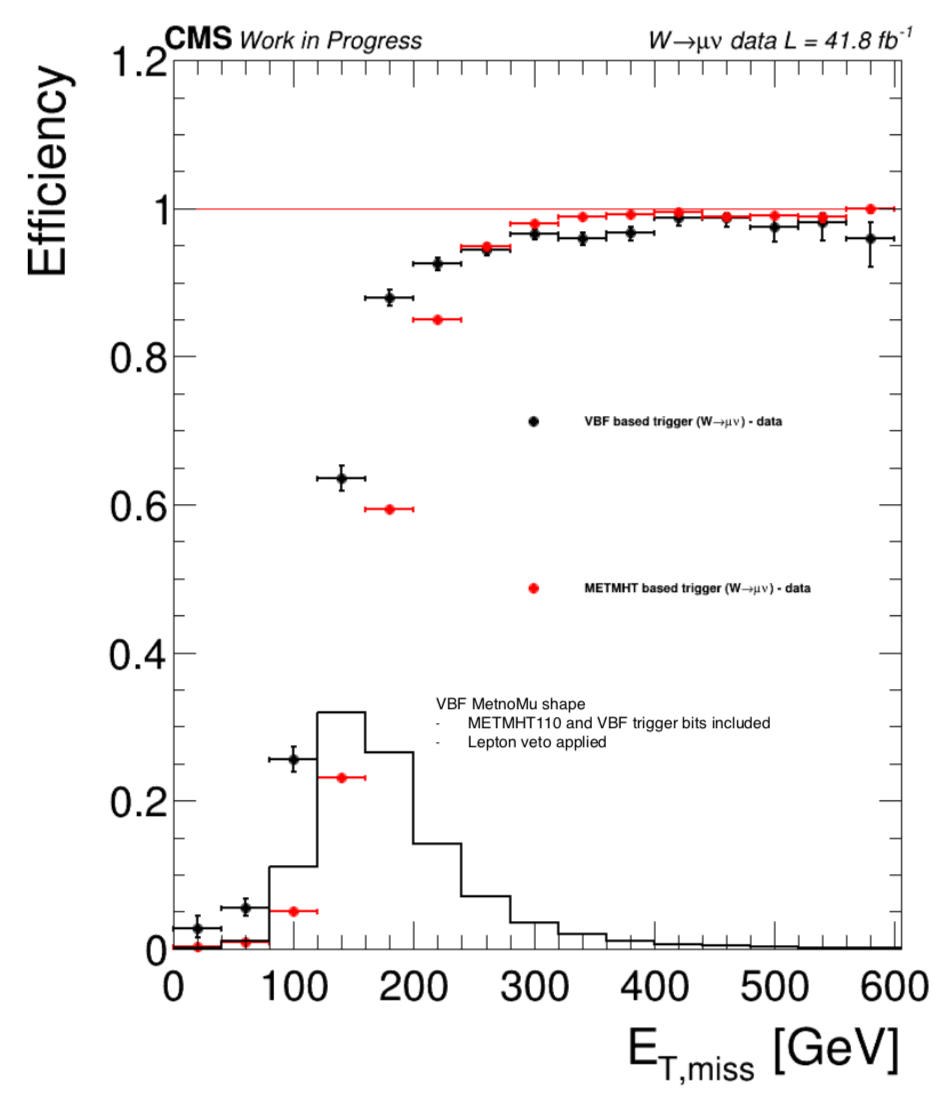
\includegraphics[width=0.5\textwidth]{Analysis_strategy/VBF_eff/2017/VBF_vs_METMHT.png}
  \caption{Comparison of efficiencies for both the MTR and VTR constructing trigger groups, presented in $E_{T,miss}$ bins. Study was performed for the 2017 era of data taking.}
  \label{fig:vbf_metmht_comp}
\end{figure}

\begin{figure}[htbp]
  \centering
    \subfigure[$E_{T,miss}$ - 2017]{
    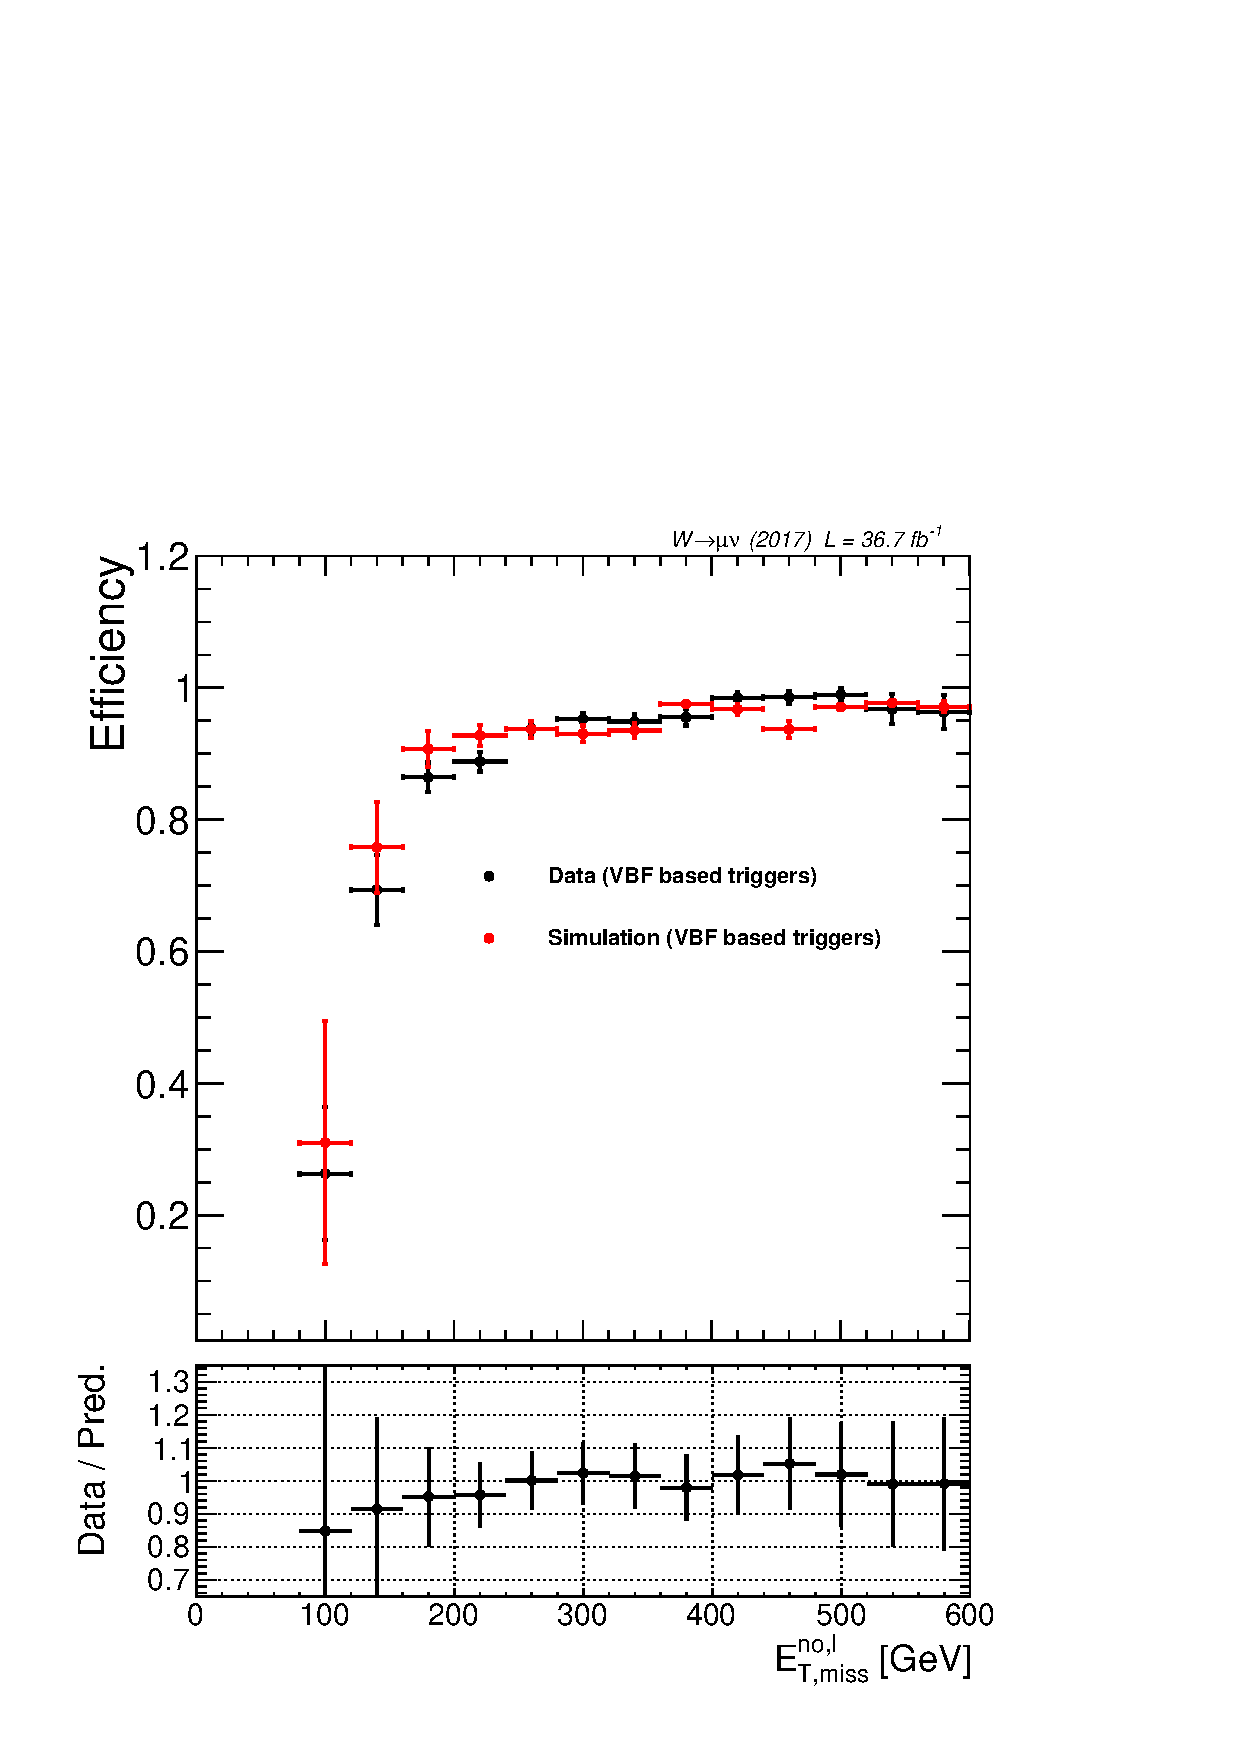
\includegraphics[width=0.45\textwidth]{Analysis_strategy/VBF_eff/MetNoMuVBF_2017.pdf}
    }
    \subfigure[$E_{T,miss}$ - 2018]{
    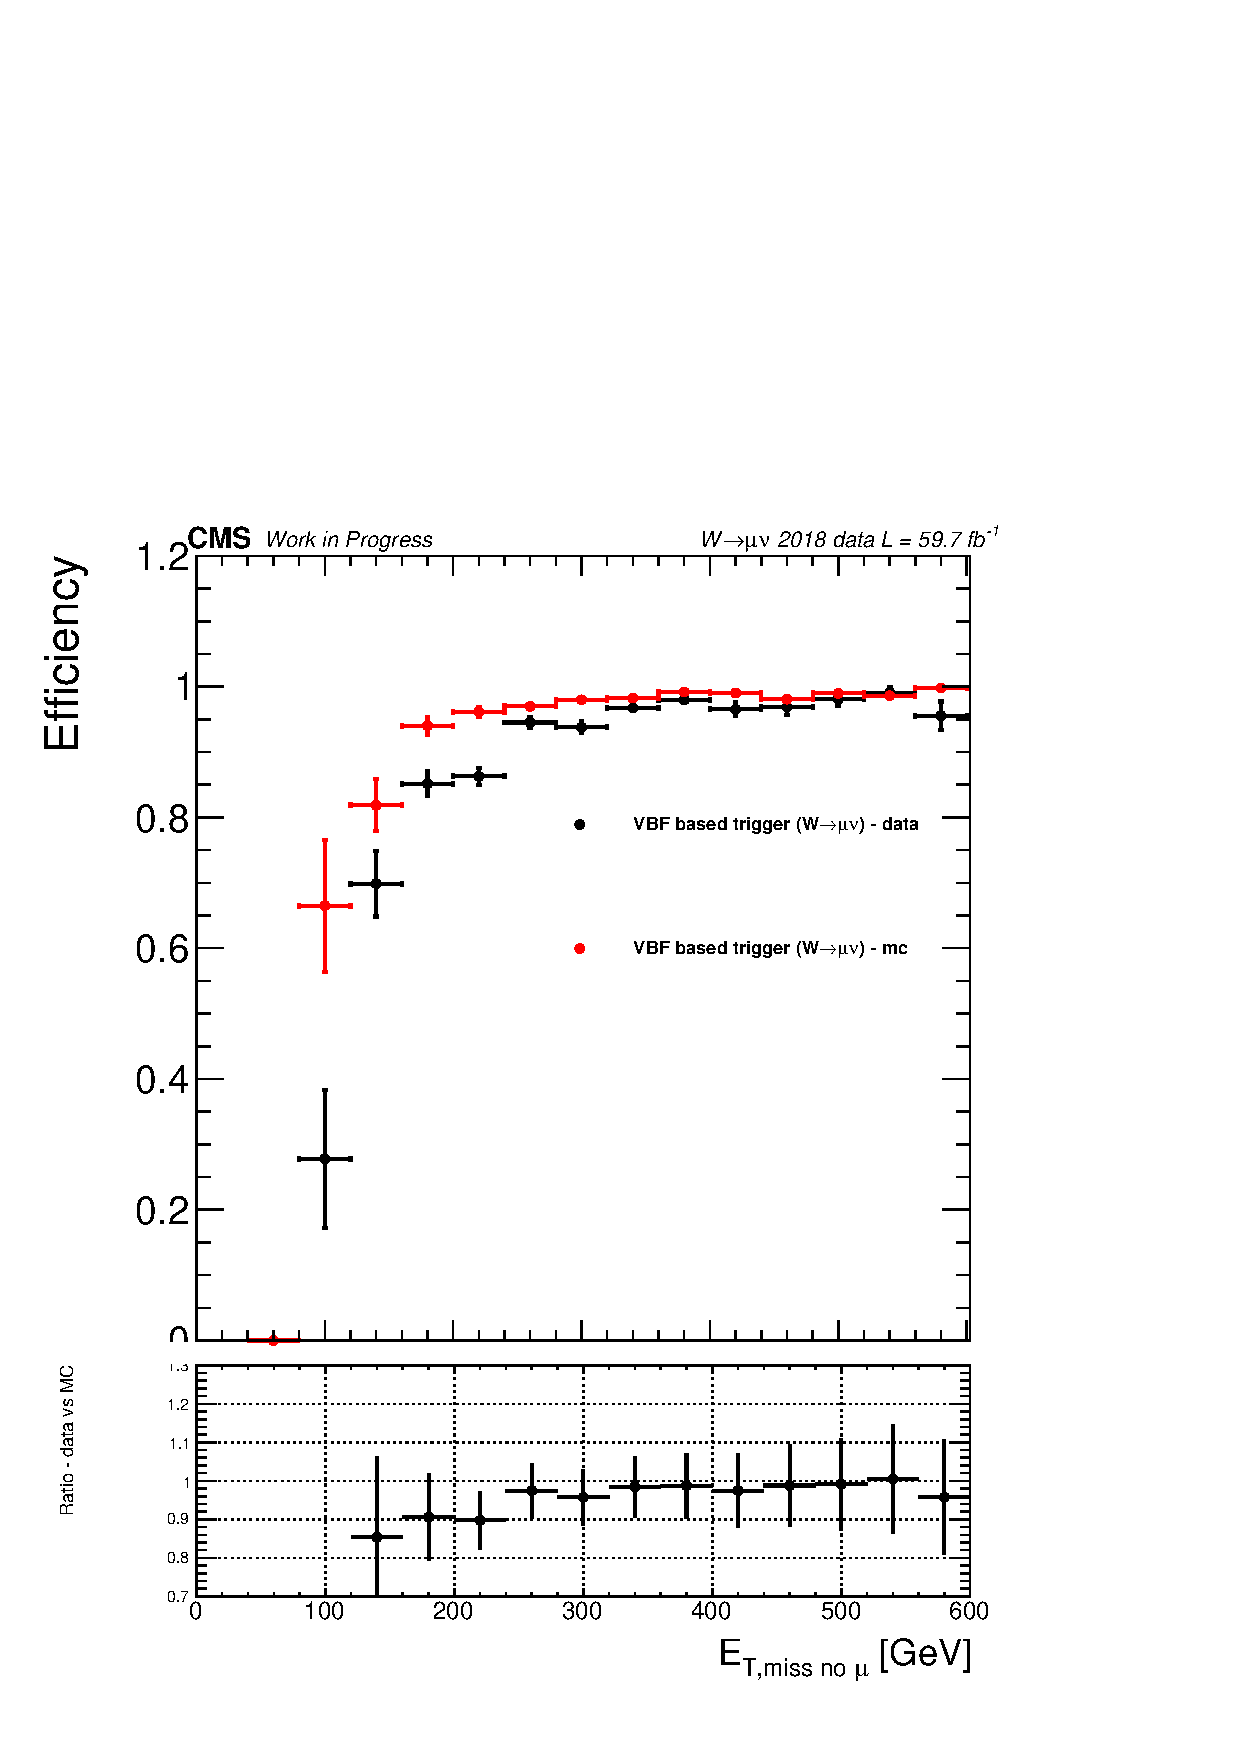
\includegraphics[width=0.45\textwidth]{Analysis_strategy/VBF_eff/MetNoMuVBF_2018.pdf}
    }
  \caption{Trigger efficiency of the logical OR of both VBF triggers, presented in $E_{T,miss}$ measured using the full VTR selection requirements for both 2017 (left) and 2018 (right) eras.}
  \label{fig:vbf_trig_eff_final}
\end{figure}

\subsection{Performance of the Electron and Photon triggers}
\hspace{10pt} For the purposes of creating dedicated control regions for V+jets background processes, in a similar vein to muon regions, a set of dedicated triggers is needed. This set is formed from three HLT paths. First algorithm employed here is the HLT\_Ele32 path. The lower $p_T>$~32~GeV threshold (35~GeV for 2018) is enabled through the implementation of the isolation requirement on the electron objects.

\hspace{10pt} Continuing with the set, a higher $p_T$ threshold electron trigger is used to help with the statistics (HLT\_Ele115), bringing the benefits of not being constrained by the isolation requirement. Finally, in order to further boost the statistics within these regions, a photon trigger (HLT\_Photon200) is brought into the setup. A logical OR of these triggers is taken as the resulting algorithm used to select events. The efficiency measurement for this set of triggers is performed using the standard "tag and probe" algorithm recommended by the E/Gamma POG~\cite{twiki:EGamma_tag_and_probe}.

\hspace{10pt} Figure~\ref{fig:hlteff_electron} shows results of these efficiency measurements for data collected during 2017 and 2018. The usage of the aforementioned information requires a special attention when forming the scale factors (SFs). Depending on the number of electrons they are defined as:
\begin{equation}
    SF = \frac{1-\prod\limits_{i}(1-\text{efficiency}_{data})}{1-\prod\limits_{i}(1-\text{efficiency}_{simulation})},
\end{equation}
where the iteration goes over each electron in the collection, allowing for easier usage when defining both electron regions.

\begin{figure}[hbtp]
\begin{center}
    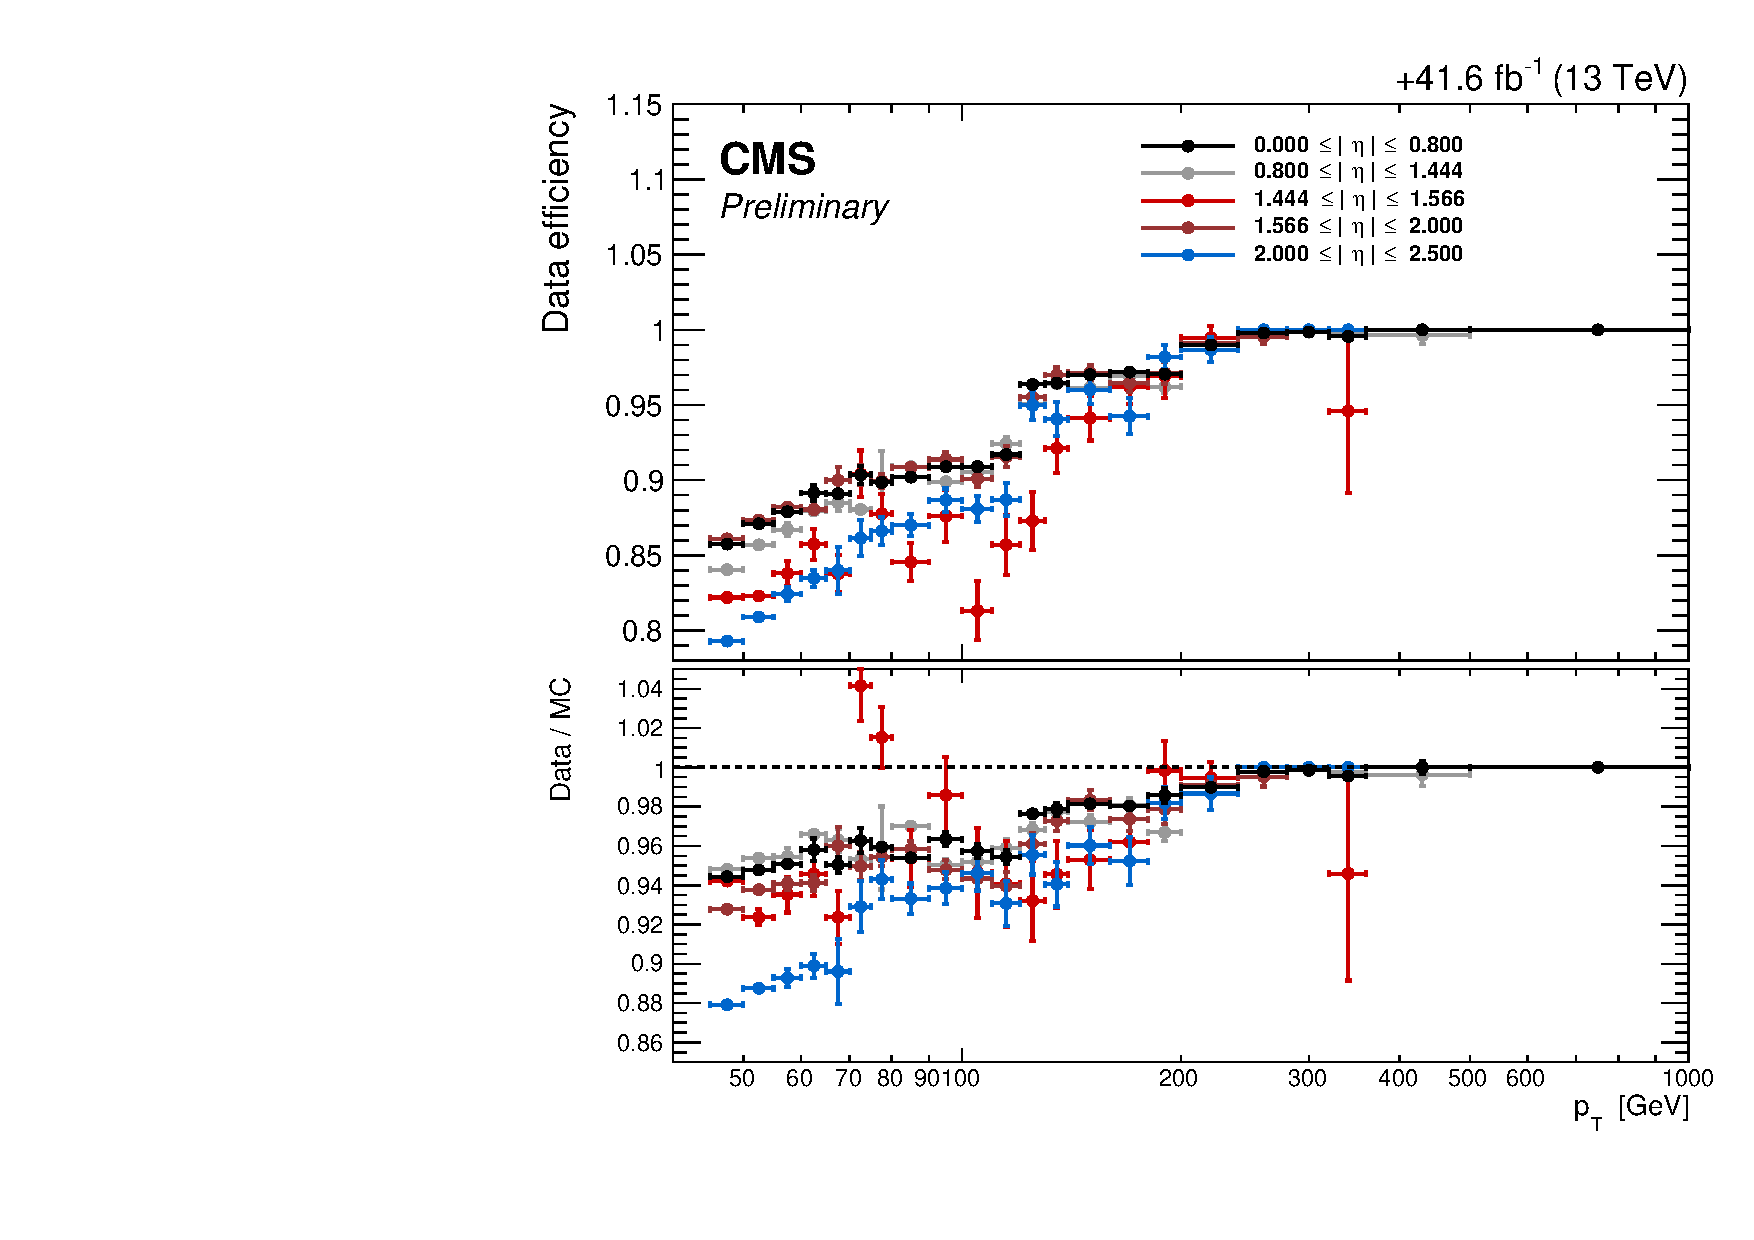
\includegraphics[width=0.45\textwidth]{Analysis_strategy/Electron_triggers/electron_trig_eff_2017.pdf}
    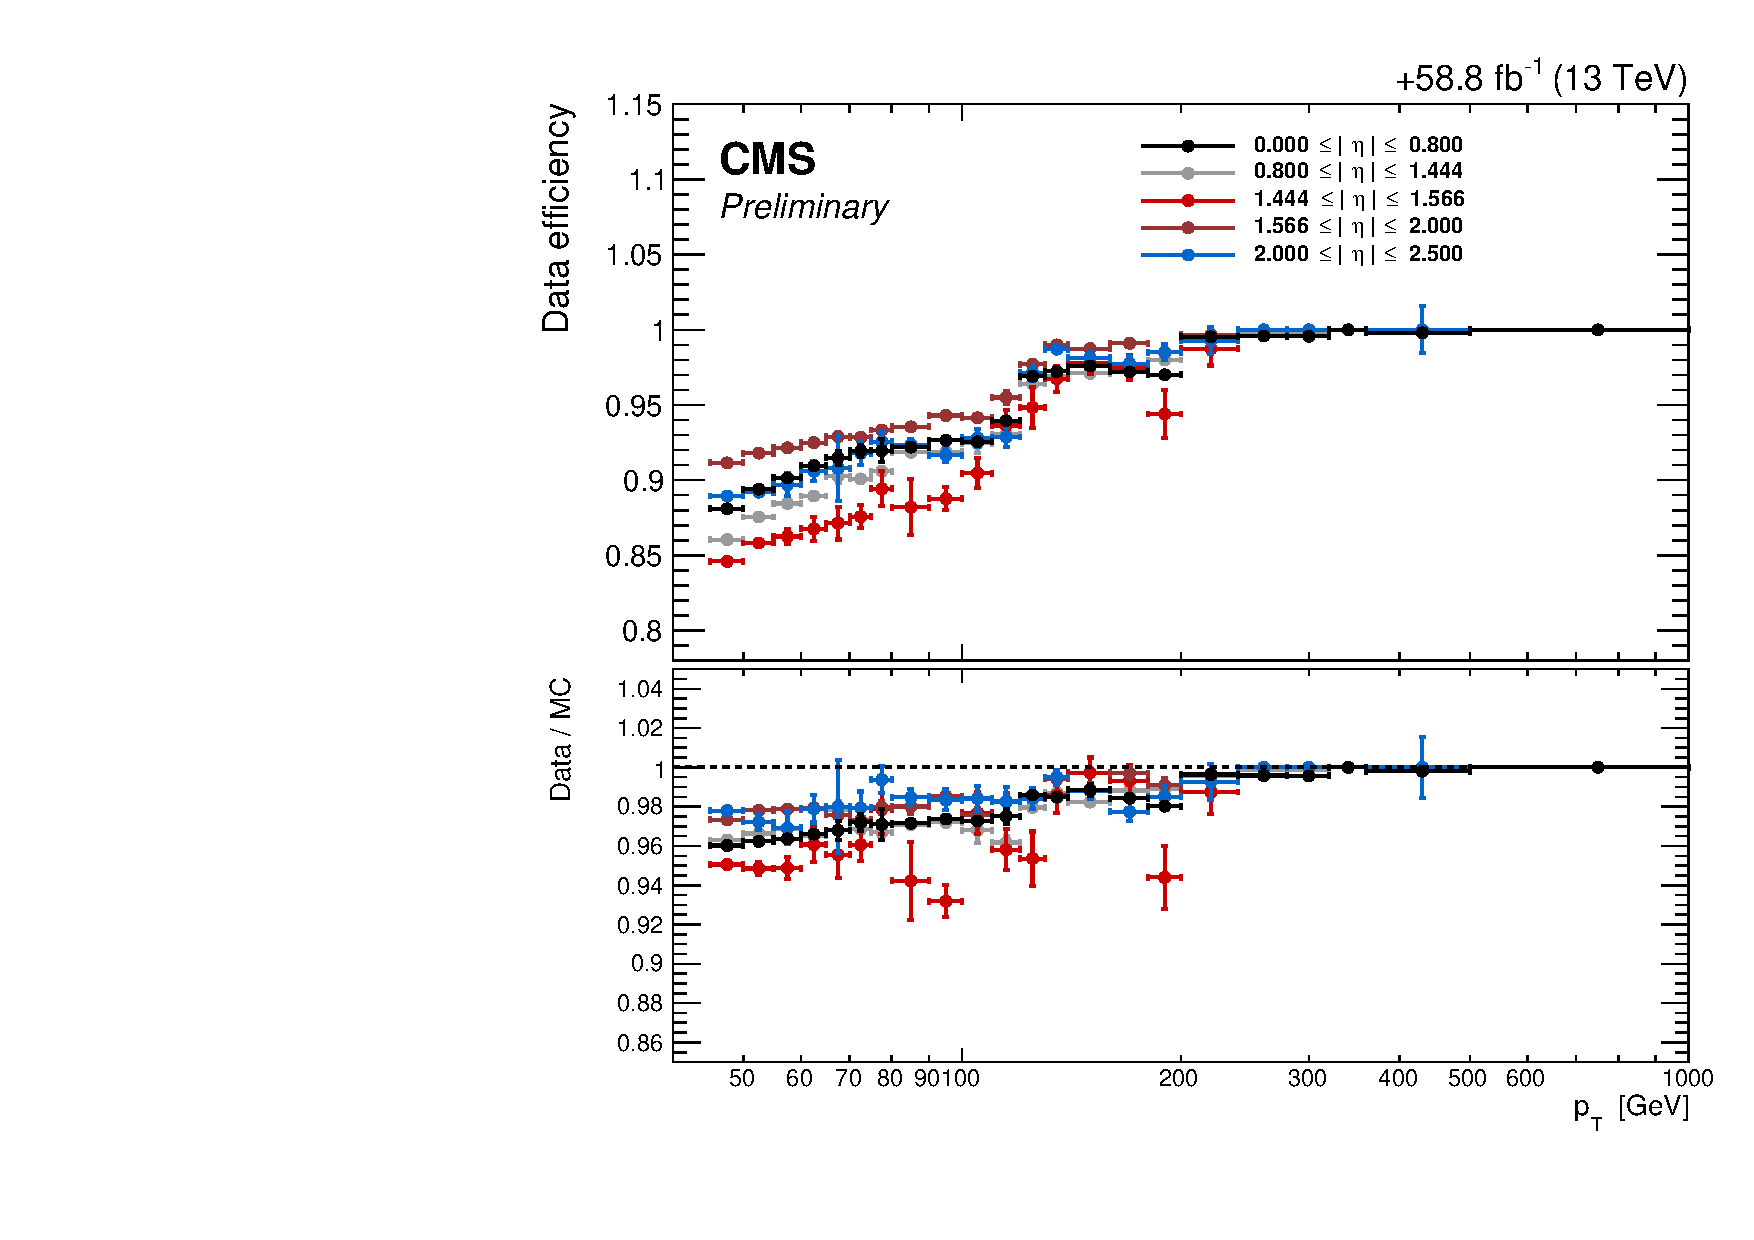
\includegraphics[width=0.45\textwidth]{Analysis_strategy/Electron_triggers/electron_trig_eff_2018.pdf}
    \caption{Efficiencies of the logical OR of the three aforementioned triggers used to select electron events for 2017 (top) and 2018 (bottom) as a function of the electron transverse momentum (separated into several categories in electron $|\eta|$)~\cite{note:AN_19_257}.}
    \label{fig:hlteff_electron}
 \end{center}
 \end{figure}

\section{Data Quality Issues}
\label{sec:data_quality}
\hspace{10pt} Midway during the 2018 era of data taking, an incident occurred at the CMS experiment, leaving a part of the HE unresponsive. In terms of detector geometry, this meant that no HCAL information was available in the $-90^\circ<\phi<-50^\circ$ and $-3.0<\eta<-1.4$ region (HE sectors 15/16). This has plagued $\sim$65~\% of the collected data during this era and has caused major concerns about its impact on the analysis. This effect was observed and treated in one of the control regions (more about that in Section~\ref{sec:single_electron}), but the main worry was coming from the SR. In order to be able to derive a proper mitigation for this effect, a blueprint involving unblinding 1/5th of the data was approved. It allowed for a look into "safe" variables that would show the effect of this problem, while not being one of the main dijet variables (removing the possibility of a biased strategy).

\hspace{10pt} Additional motivation for this approach was also fueled by the desire to check for the appearance of the effect called the jet "horns". It is represented with a large number of events with jets being reconstructed in the $2.8<|\eta|<3.2$ region for data only, being omitted from the simulation modeling. The following paragraphs will summarise the strategies that were the result of this unblinding.

\subsection{Jet "horns" mitigation}
\hspace{10pt} One of the problems associated to the studies focused on jets is the appearance of a large amount of low quality jets in data for a certain $|\eta|$ range, not properly represented in the simulation. The range of this effect, covering the $2.8<|\eta|<3.2$ region, creates issues for this analysis as well, unfortunately for both eras. Figure~\ref{fig:jet_eta_preHornCut} shows that even the PU jet ID, imposed when creating analysis level jets, was not enough to diminish this effect (even though this was enough to eliminate this occurrence in the dedicated control regions). The effect is more prominently seen for the the leading jet compared to the subleading jet, which is a clear consequence of the high $E_{T,miss}$ selection requirement (being computed from higher $p_T$ jet in the former case).


\begin{figure}[htbp]
  \centering
    \subfigure[$\eta_{j1}$ - MTR]{
    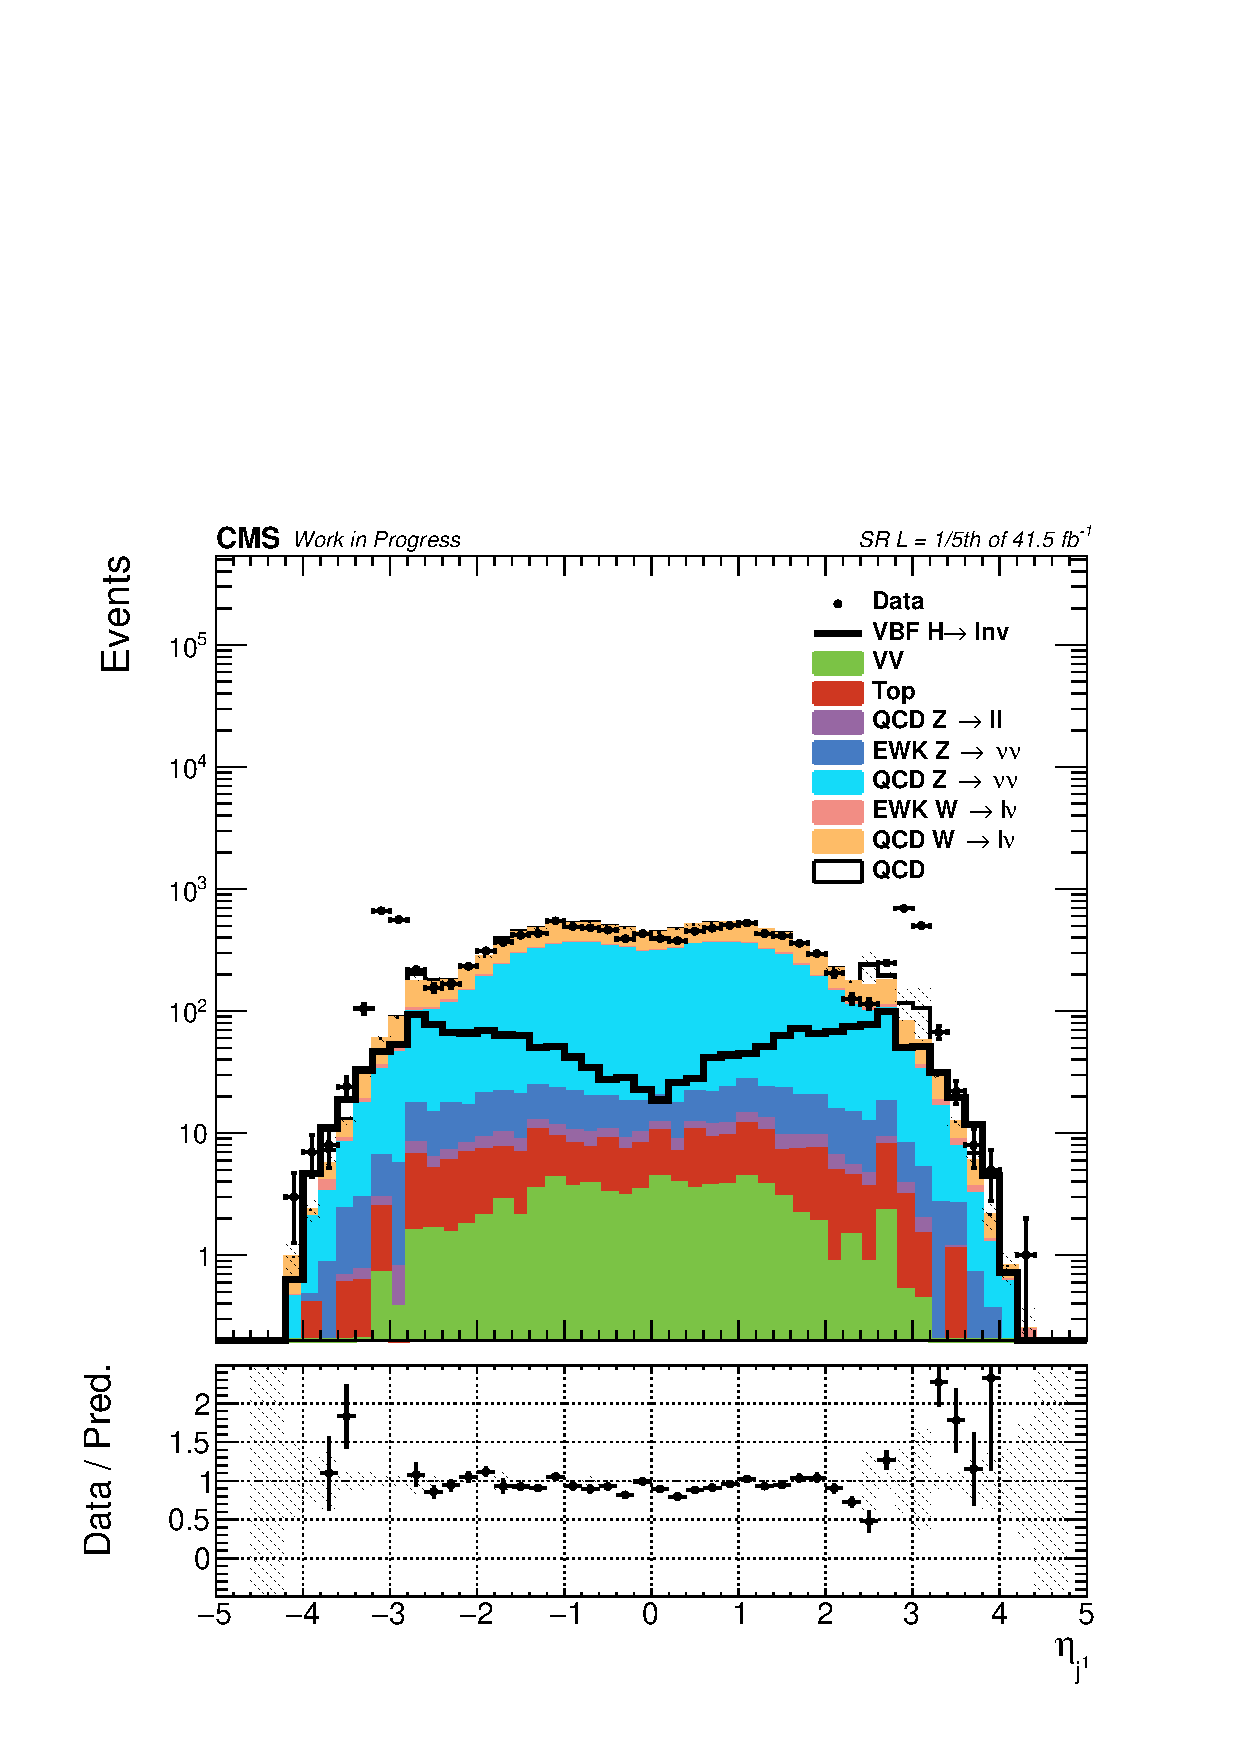
\includegraphics[width=0.49\textwidth]{Analysis_strategy/2017_preHornCut/Leading_jet_eta_log.pdf}
    }
    \subfigure[$\eta_{j2}$ - MTR]{
    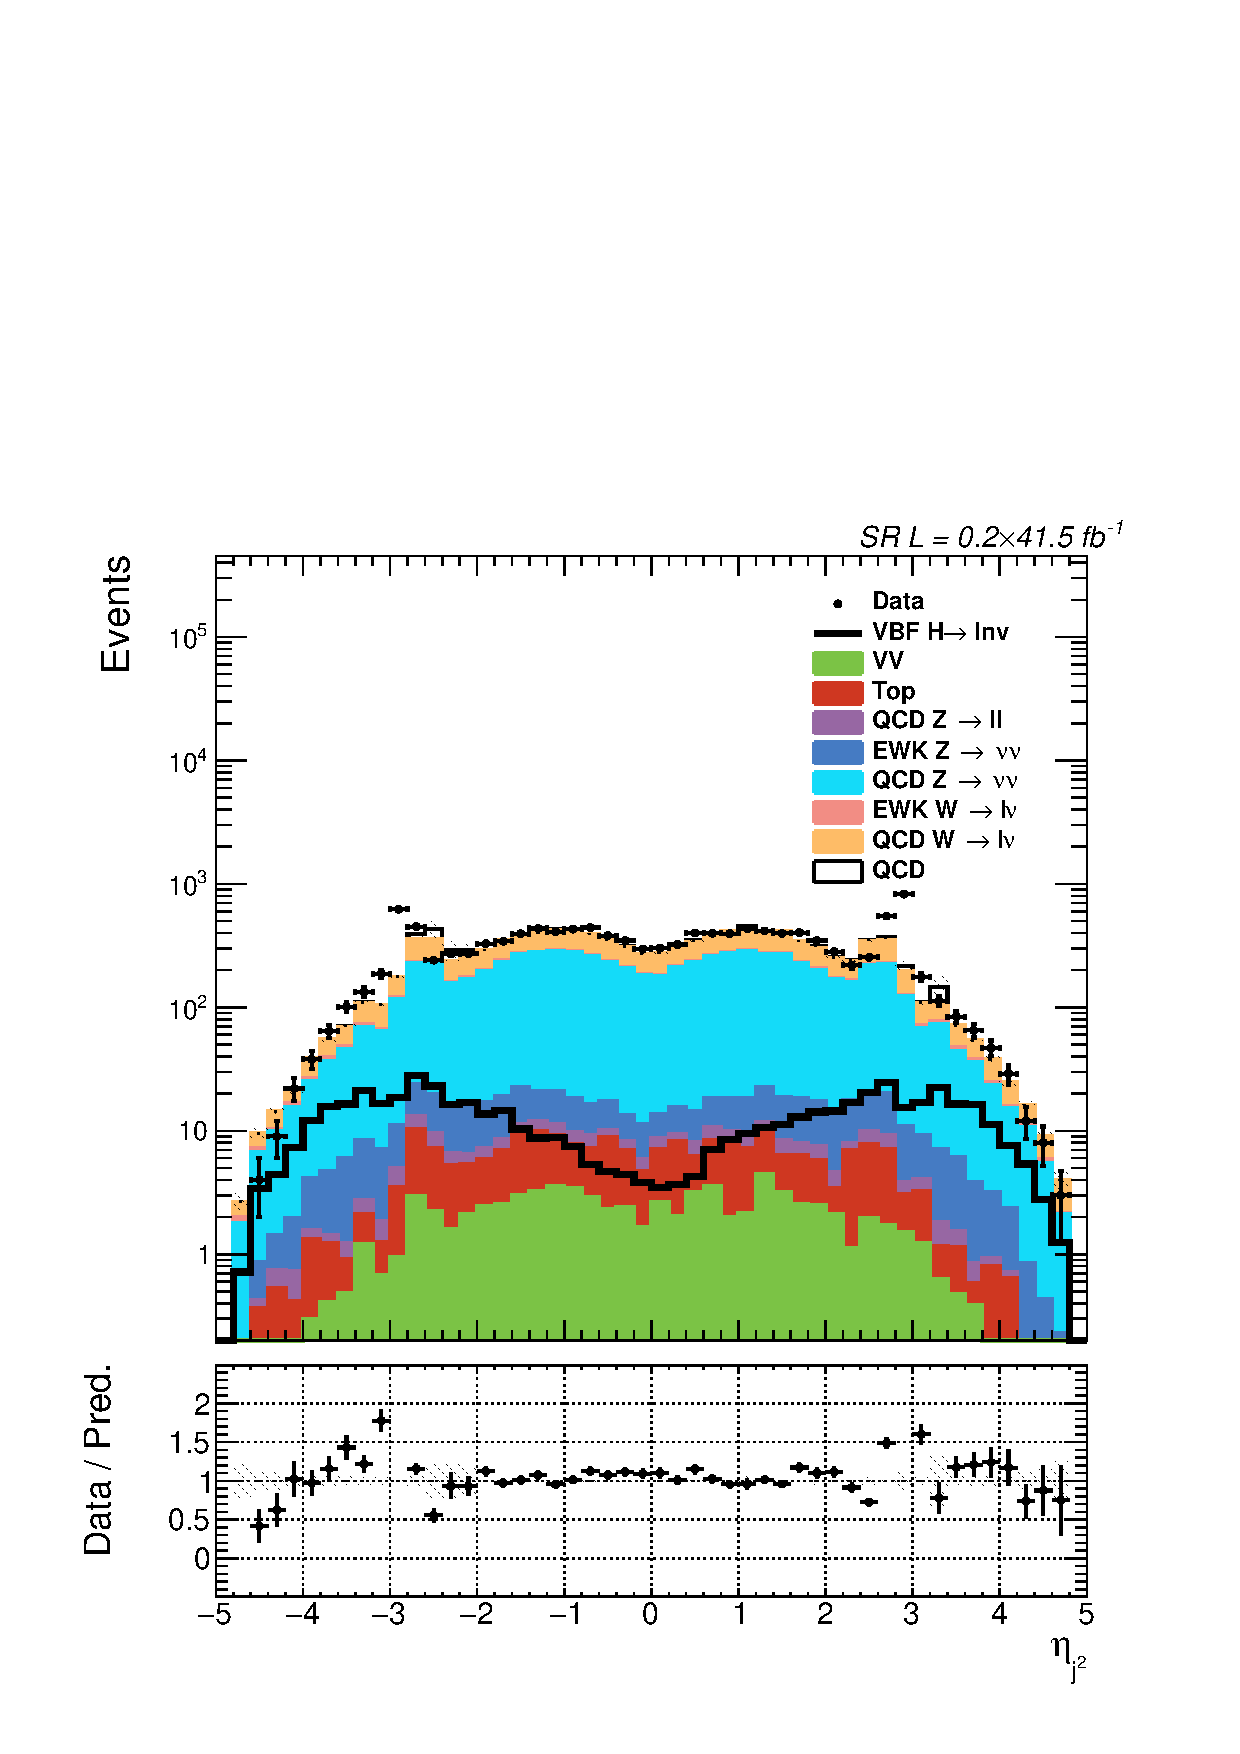
\includegraphics[width=0.49\textwidth]{Analysis_strategy/2017_preHornCut/Subleading_jet_eta_log.pdf}
    }\\
    \subfigure[$\eta_{j1}$ - VTR]{
    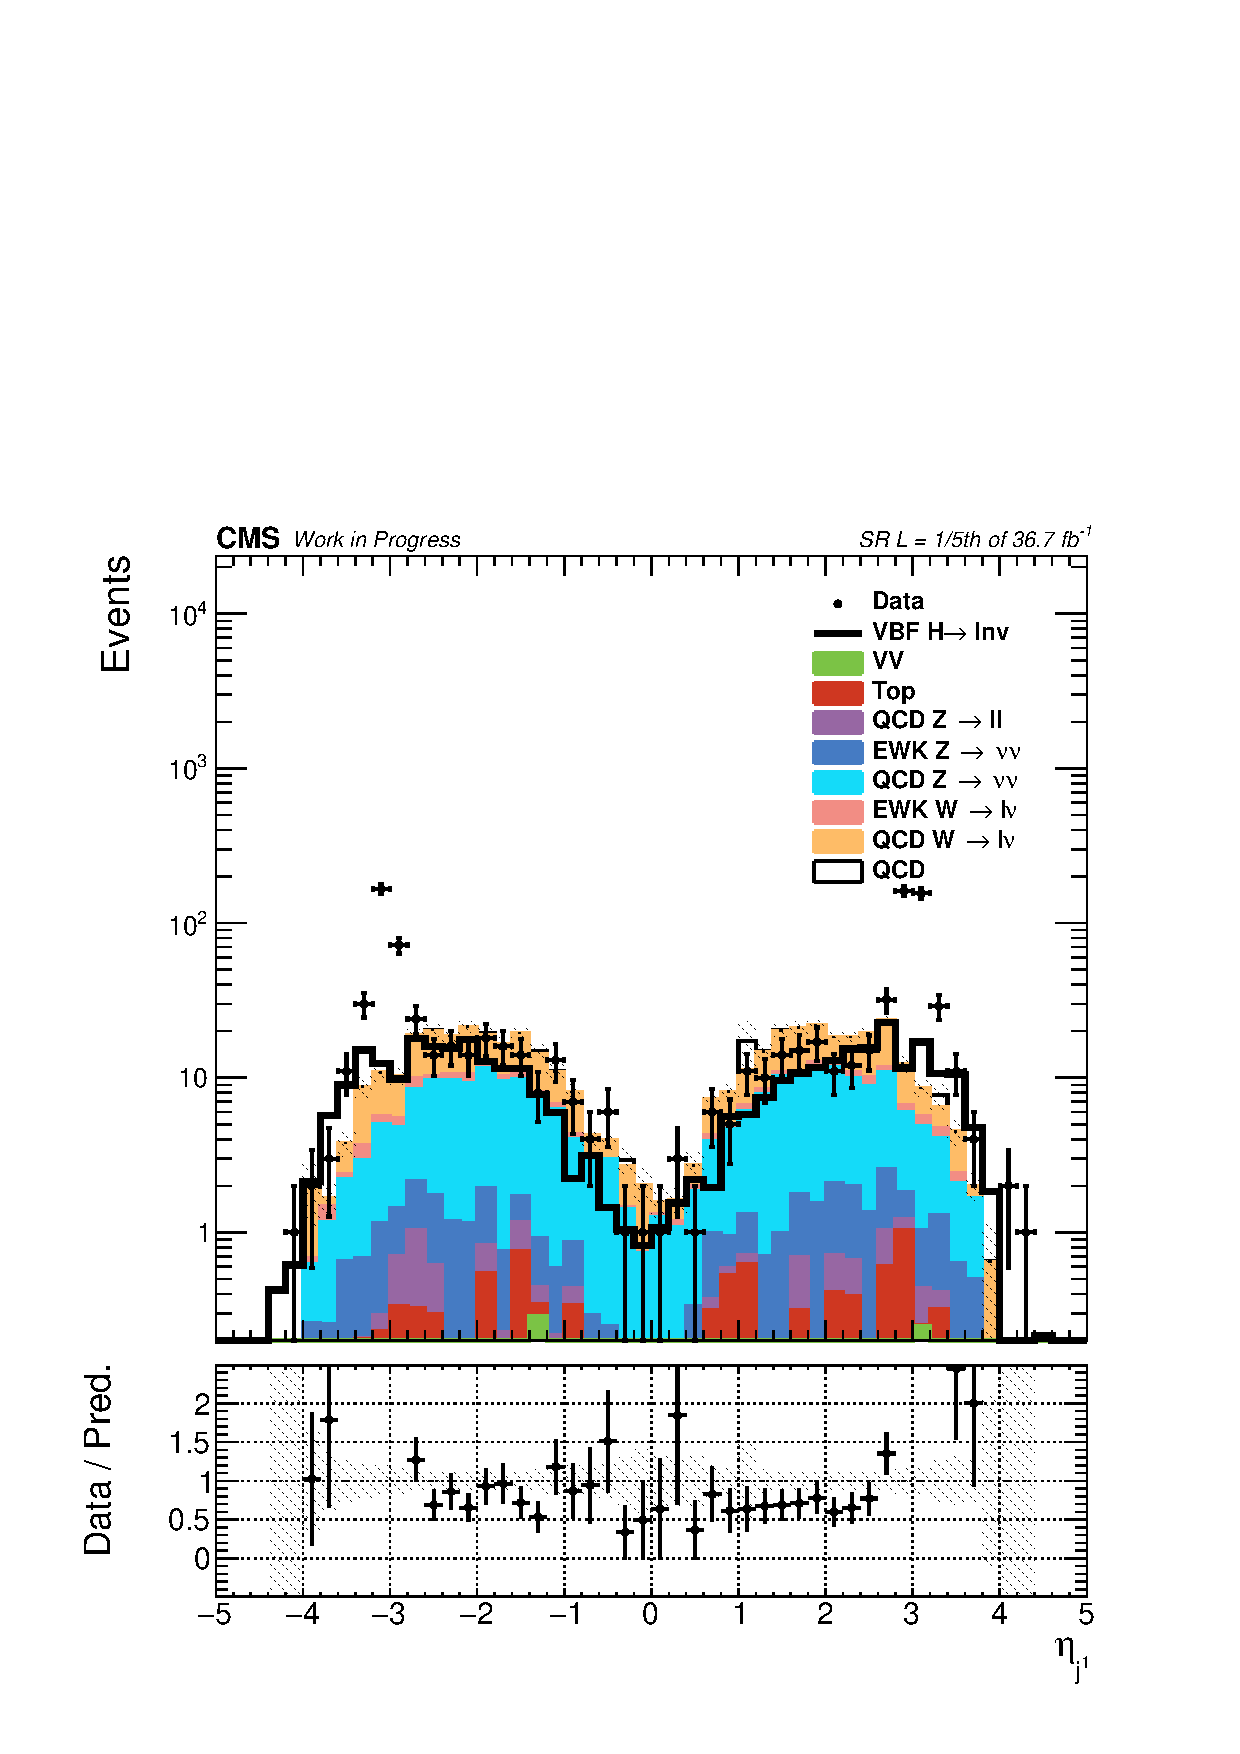
\includegraphics[width=0.49\textwidth]{Analysis_strategy/2017_preHornCut/VTRLeading_jet_eta_log.pdf}
    }
    \subfigure[$\eta_{j2}$ - VTR]{
    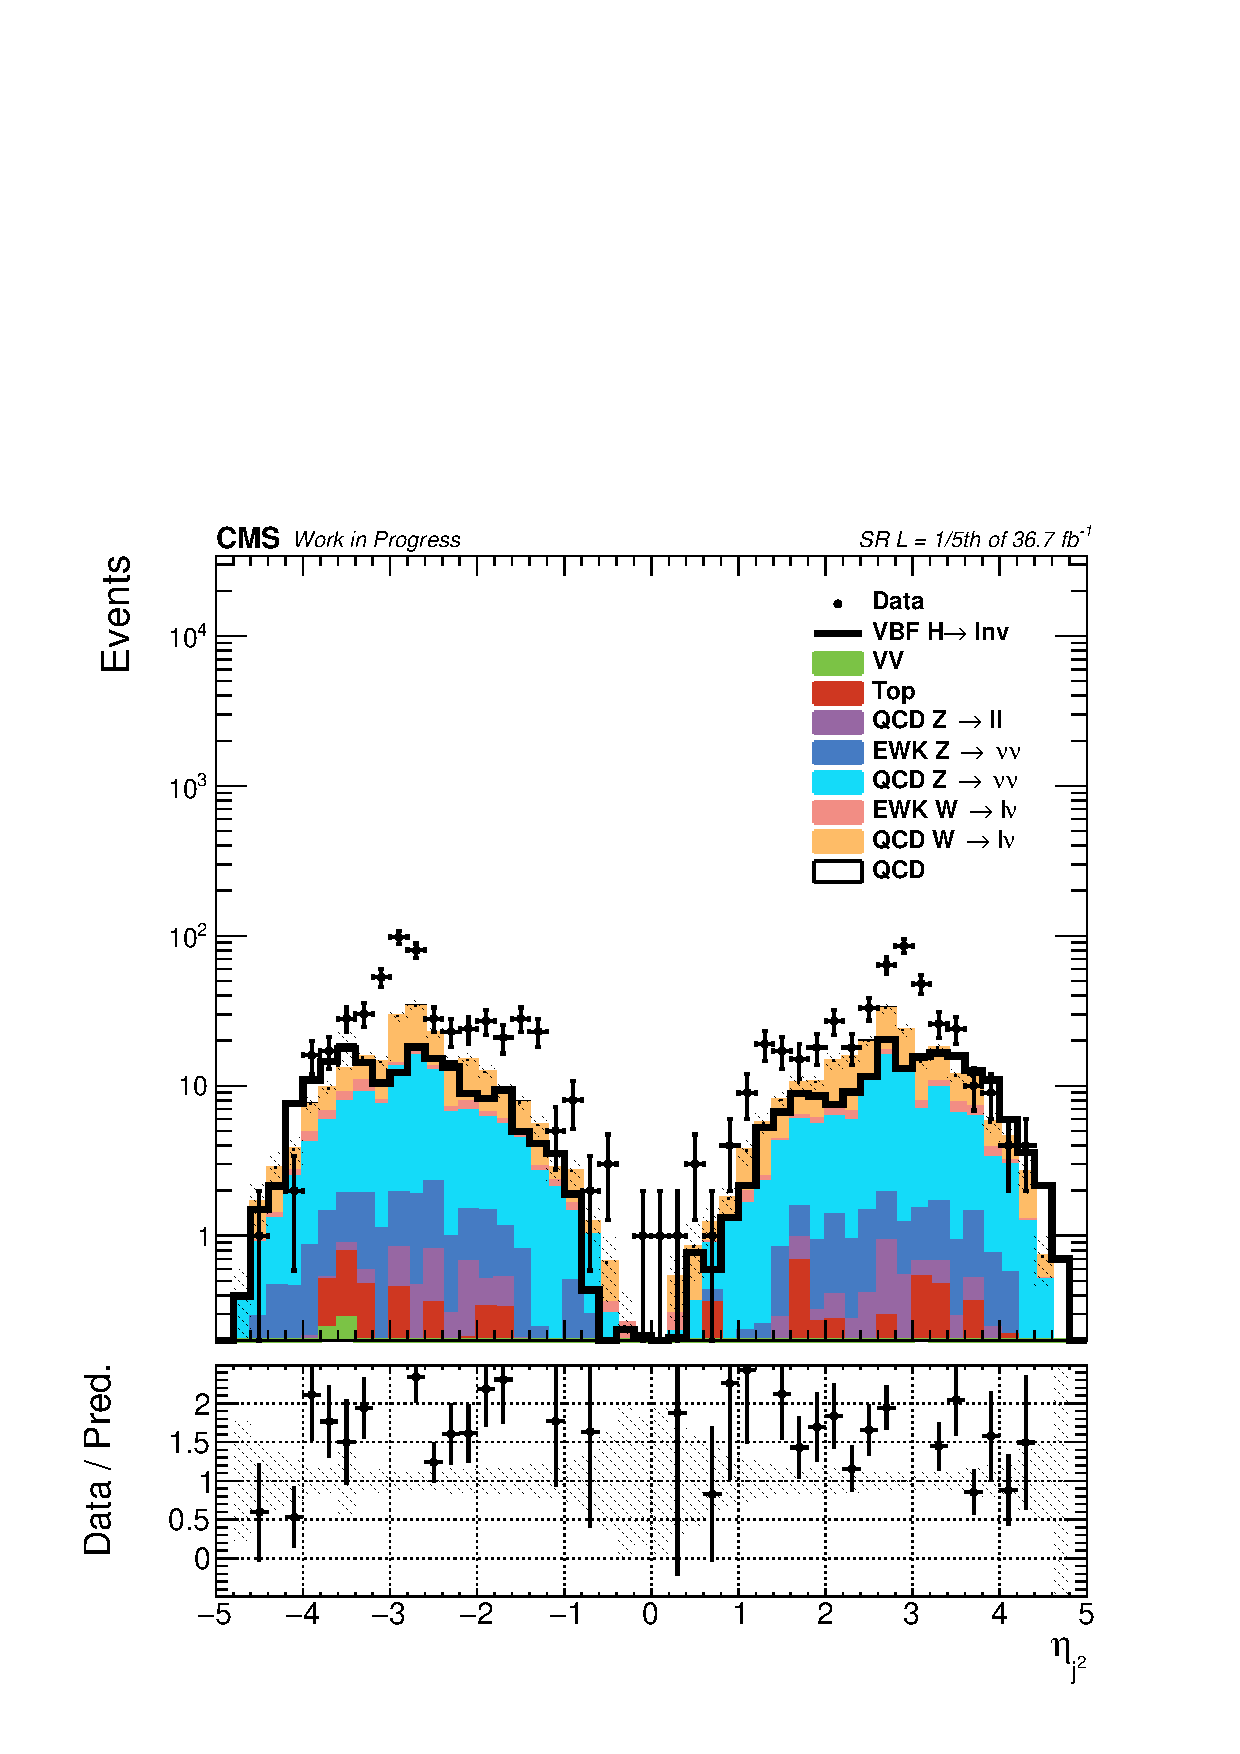
\includegraphics[width=0.49\textwidth]{Analysis_strategy/2017_preHornCut/VTRSubleading_jet_eta_log.pdf}
    }
  \caption{Distributions of $\eta_{j1}$ (left) and $\eta_{j2}$ (right) variables in the signal region after the unbinding of 1/5th of the 2017 data. Both MTR (top) and VTR (bottom) categories are presented.}
  \label{fig:jet_eta_preHornCut}
\end{figure}




\hspace{10pt} In order to look for a proper mitigation approach, various techniques of computing the $E_{T, miss}$ were checked (based on the set of particles entering the computation). As explained in Section~\ref{sec:objects}, the offline $E_{T,miss}$ is computed through the usage of all PF objects. A restriction, allowing only objects which are registered by the tracker into the calculation of $E_{T,miss}$, would give a better handle on the problem, as the difference between the two includes the neutrally charged PF candidates. This difference is well accounted for in the simulation, leading to the conclusion that any significant deviations from the expected behaviour can be associated largely to these low quality jets.

\hspace{10pt} Figure~\ref{fig:met_vs_tkmet_2017} shows distributions of the relative difference between the tracker ($E_{T,miss}^{~track}$) and the standard $E_{T, miss}$. It can be seen that a large deviation from the expected simulation behaviour is observed in the region where this difference is larger than 0.8. Using the aforementioned region in order to contain the jet behavior, a requirement that a jet within the 2.8~$<|\eta|<$~3.2 region has to have value of 1-$E_{T,miss}^{~track}$/$E_{T, miss}<$~0.8  was introduced into the existing set of analysis requirements for both categories.

\begin{figure}[htbp]
  \centering
    \subfigure[1-$E_{T,miss}^{~track}$/$E_{T, miss}$ - MTR]{
    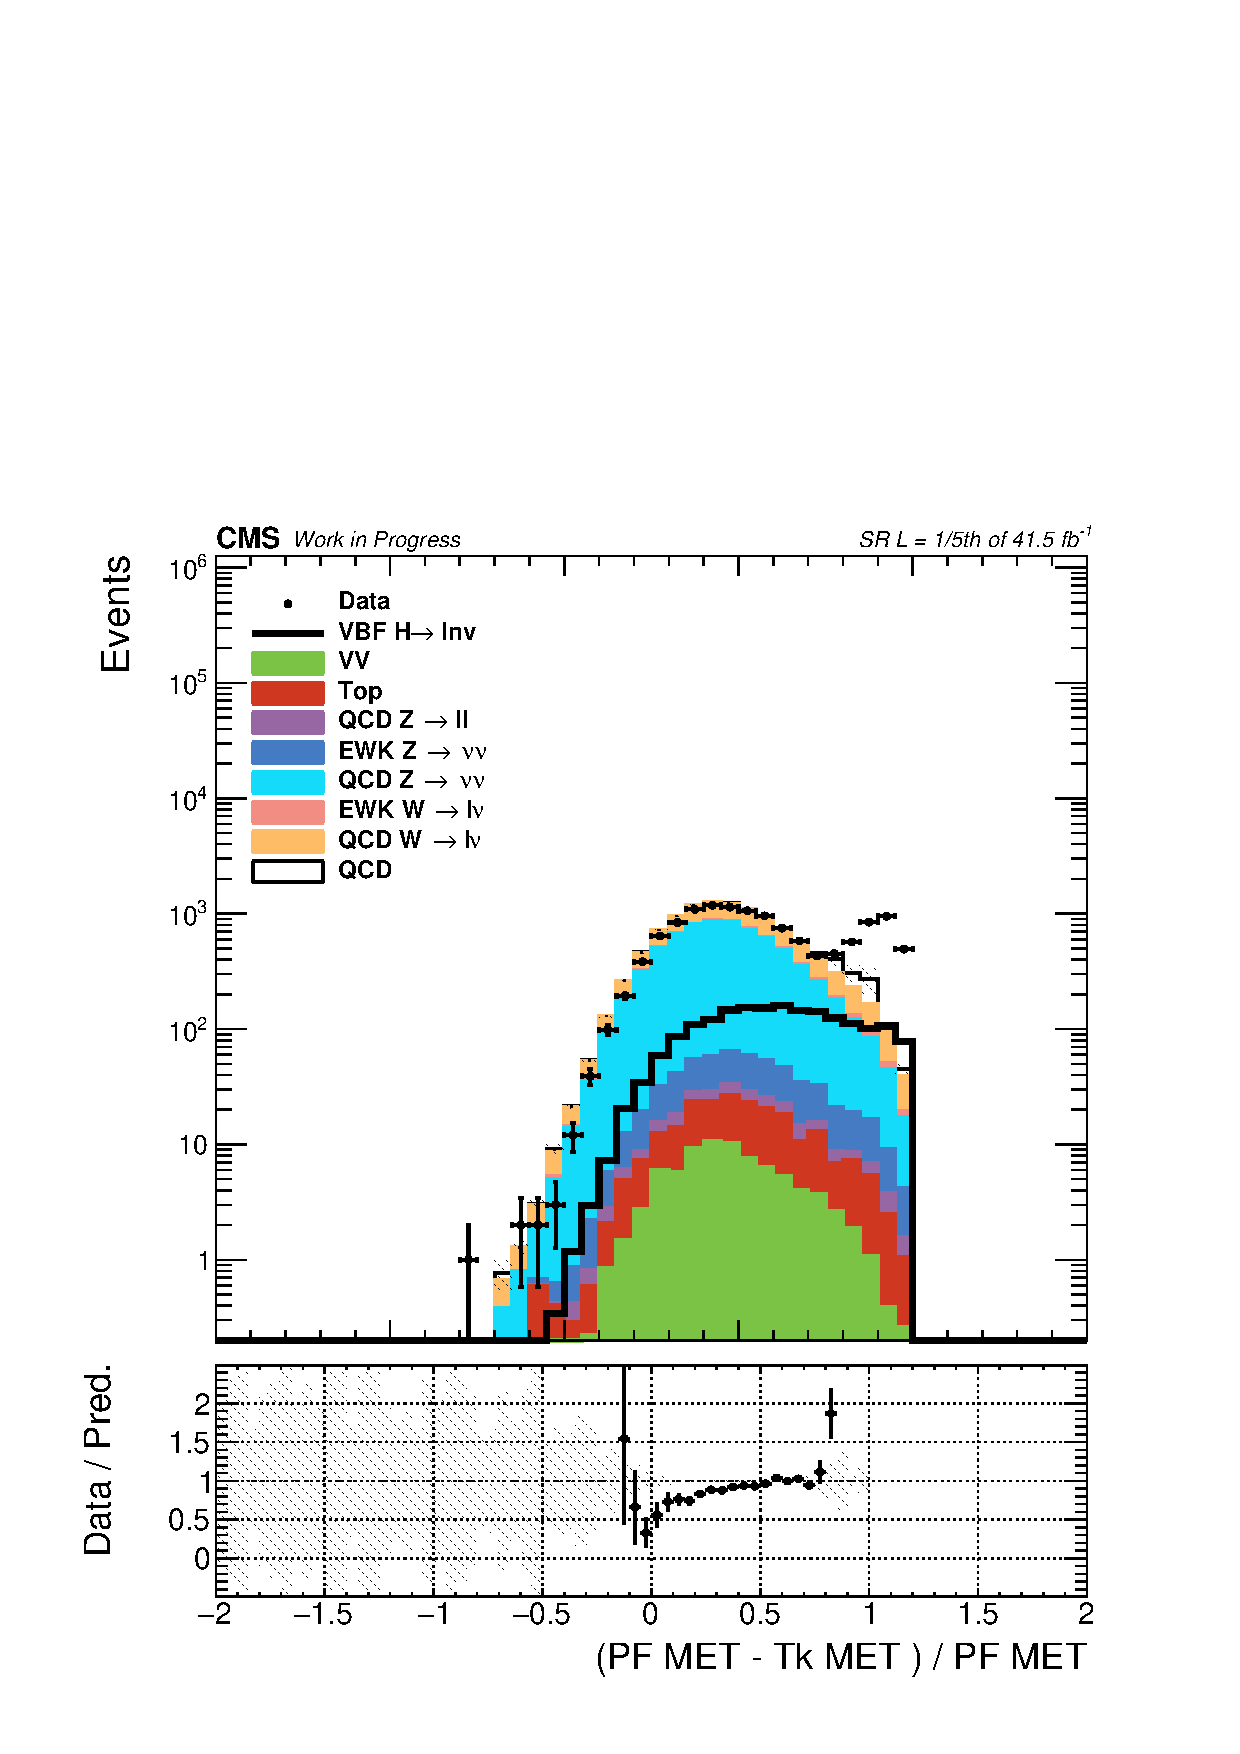
\includegraphics[width=0.49\textwidth]{Analysis_strategy/2017_preHornCut/TkMET_reldiff_MET_log.pdf}
    }
    \subfigure[1-$E_{T,miss}^{~track}$/$E_{T, miss}$ - VTR]{
    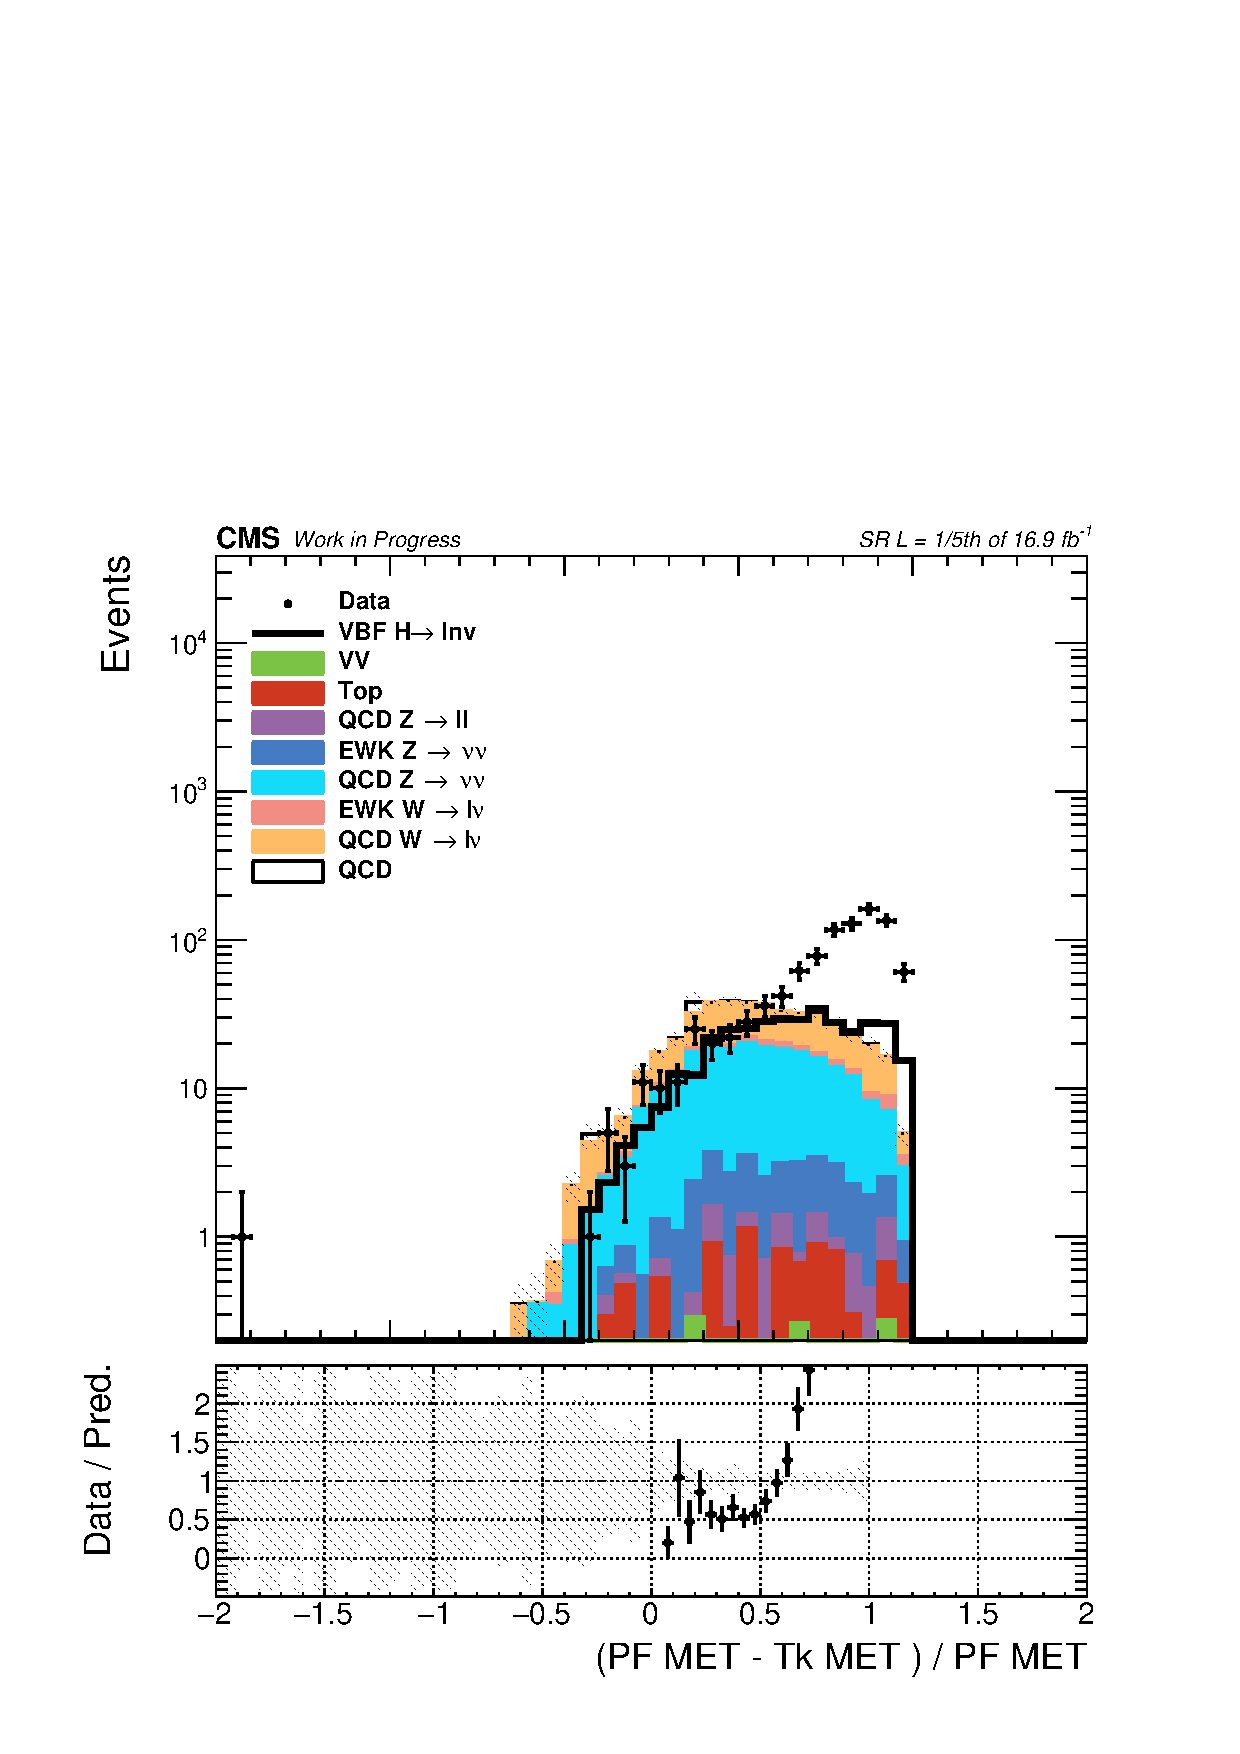
\includegraphics[width=0.49\textwidth]{Analysis_strategy/2017_preHornCut/VTRTkMET_reldiff_MET_log.pdf}
    }
  \caption{Distributions of the 1-$E_{T,miss}^{~track}$/$E_{T, miss}$ variable in the signal region after the unbinding of 1/5th of the 2017 data. Both MTR (left) and VTR categories are represented.}
  \label{fig:met_vs_tkmet_2017}
\end{figure}

\hspace{10pt} Figures~\ref{fig:jet_eta_postHornCut} and shows ~\ref{fig:2017_postHornCut_met_vs_tkmet} distribution of jet eta (for both the leading and subleading jets) and the 1-$E_{T,miss}^{~track}$/$E_{T, miss}$ relation after the inclusion of the aforementioned requirement, showcasing the mitigation power of this choice which has lead to a significantly diminished effect of jet "horns". All of the presented distributions used to illustrate this effect are related to the 2017 era, while the equivalent set representing the 2018 era is given in Appendix A. This mitigation process has led to a small loss of signal efficiency. Computed using the simulation samples of signal processes, it had impacted the VBF production with a $\sim$8~\% and gluon-fusion with a $\sim$1\% of signal efficiency loss, leading to a combined value of 4\%.

\begin{figure}[htbp]
  \centering
    \subfigure[$\eta_{j1}$ - MTR]{
    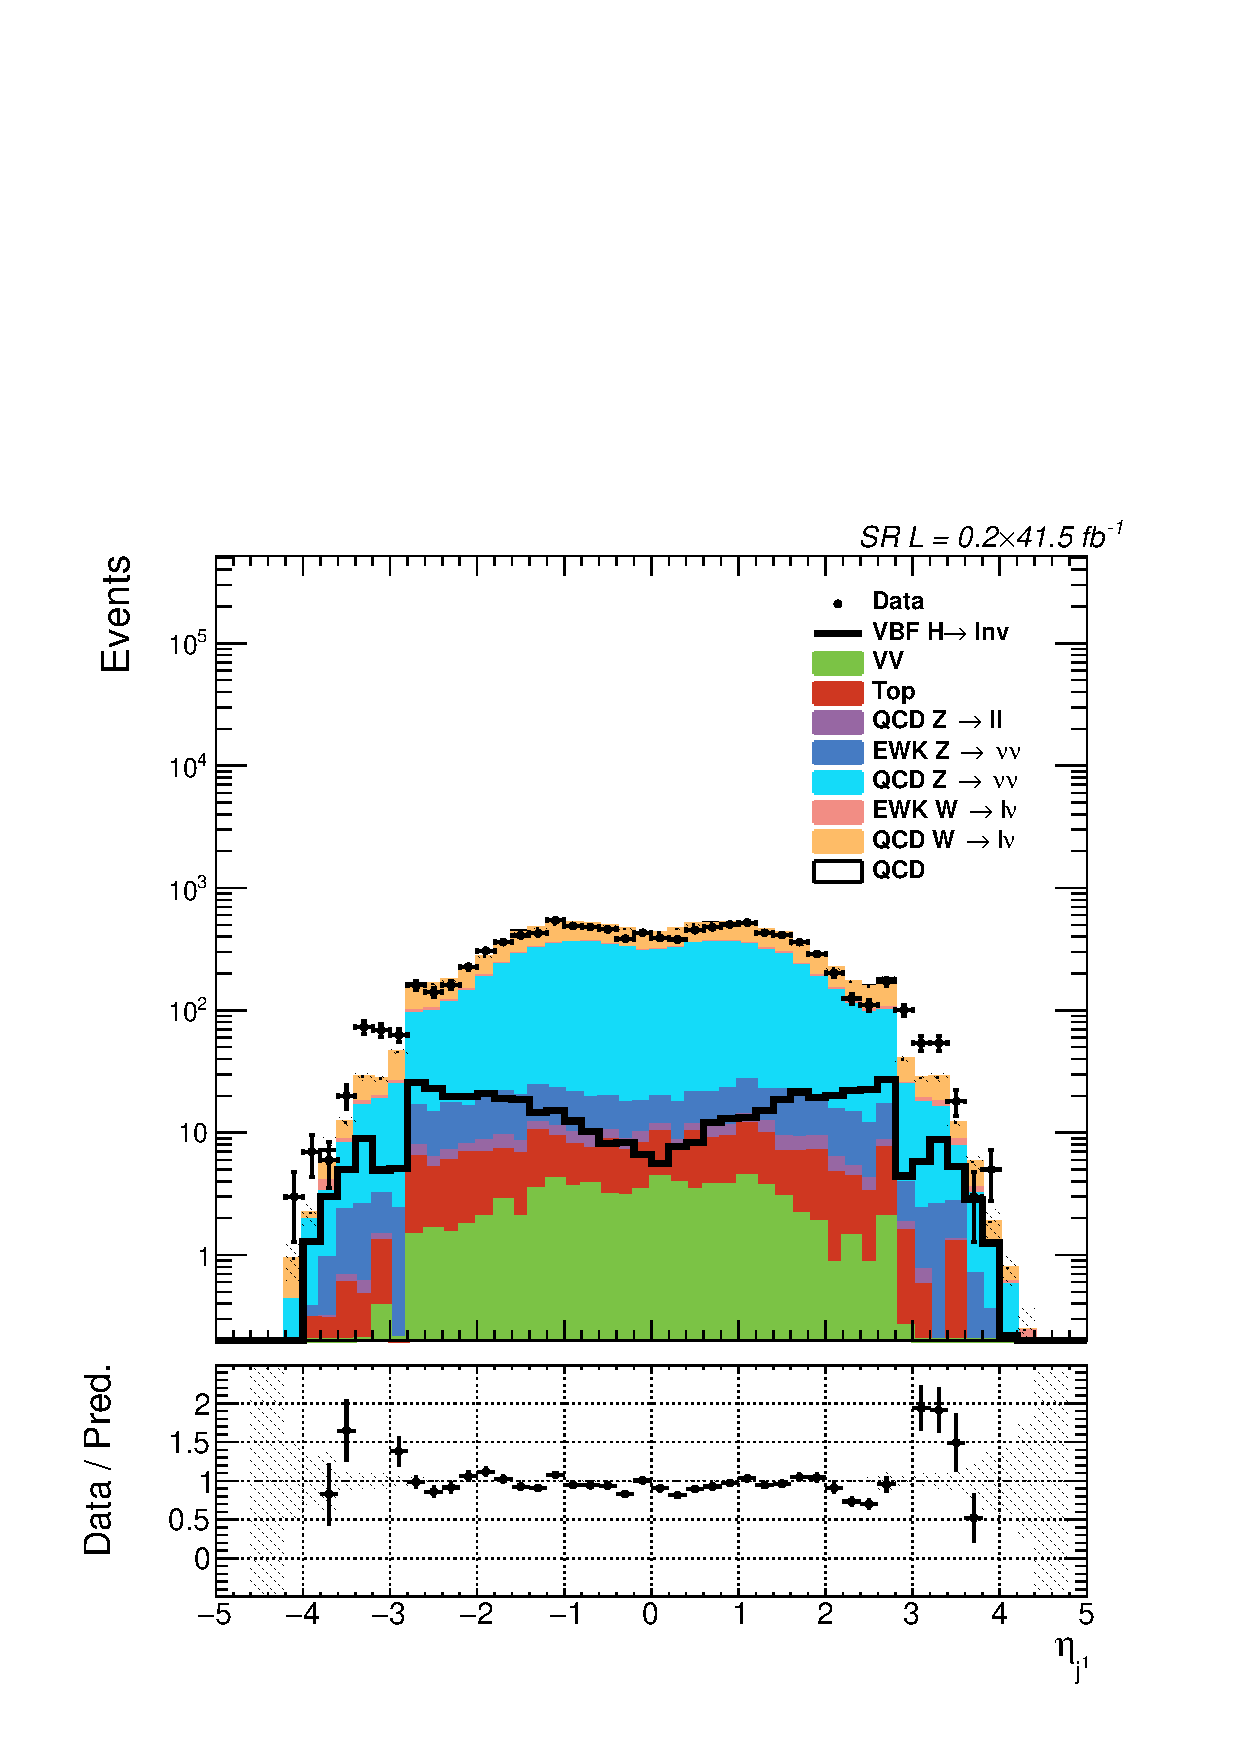
\includegraphics[width=0.49\textwidth]{Analysis_strategy/2017_postHornCut/Leading_jet_eta_log.pdf}
    }
    \subfigure[$\eta_{j2}$ - MTR]{
    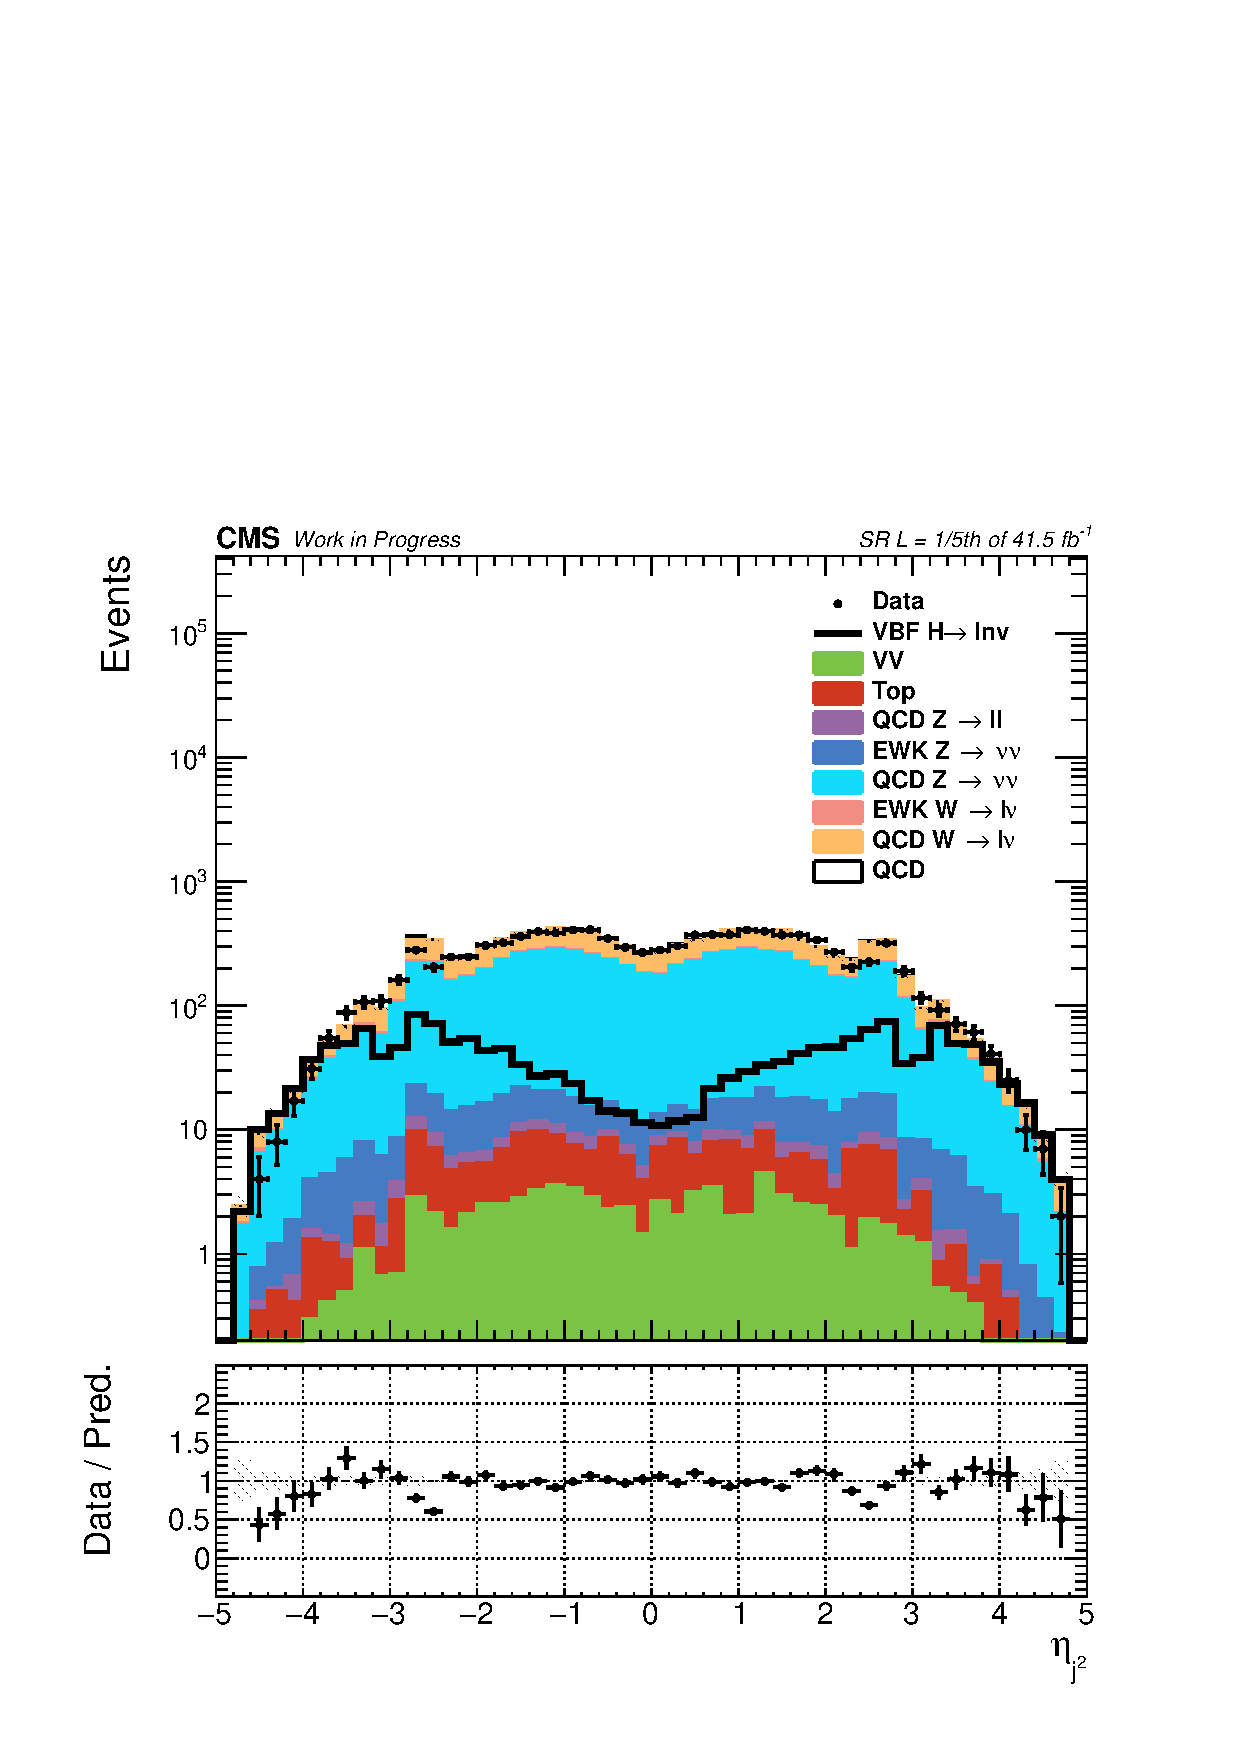
\includegraphics[width=0.49\textwidth]{Analysis_strategy/2017_postHornCut/Subleading_jet_eta_log.pdf}
    }\\
    \subfigure[$\eta_{j1}$ - VTR]{
    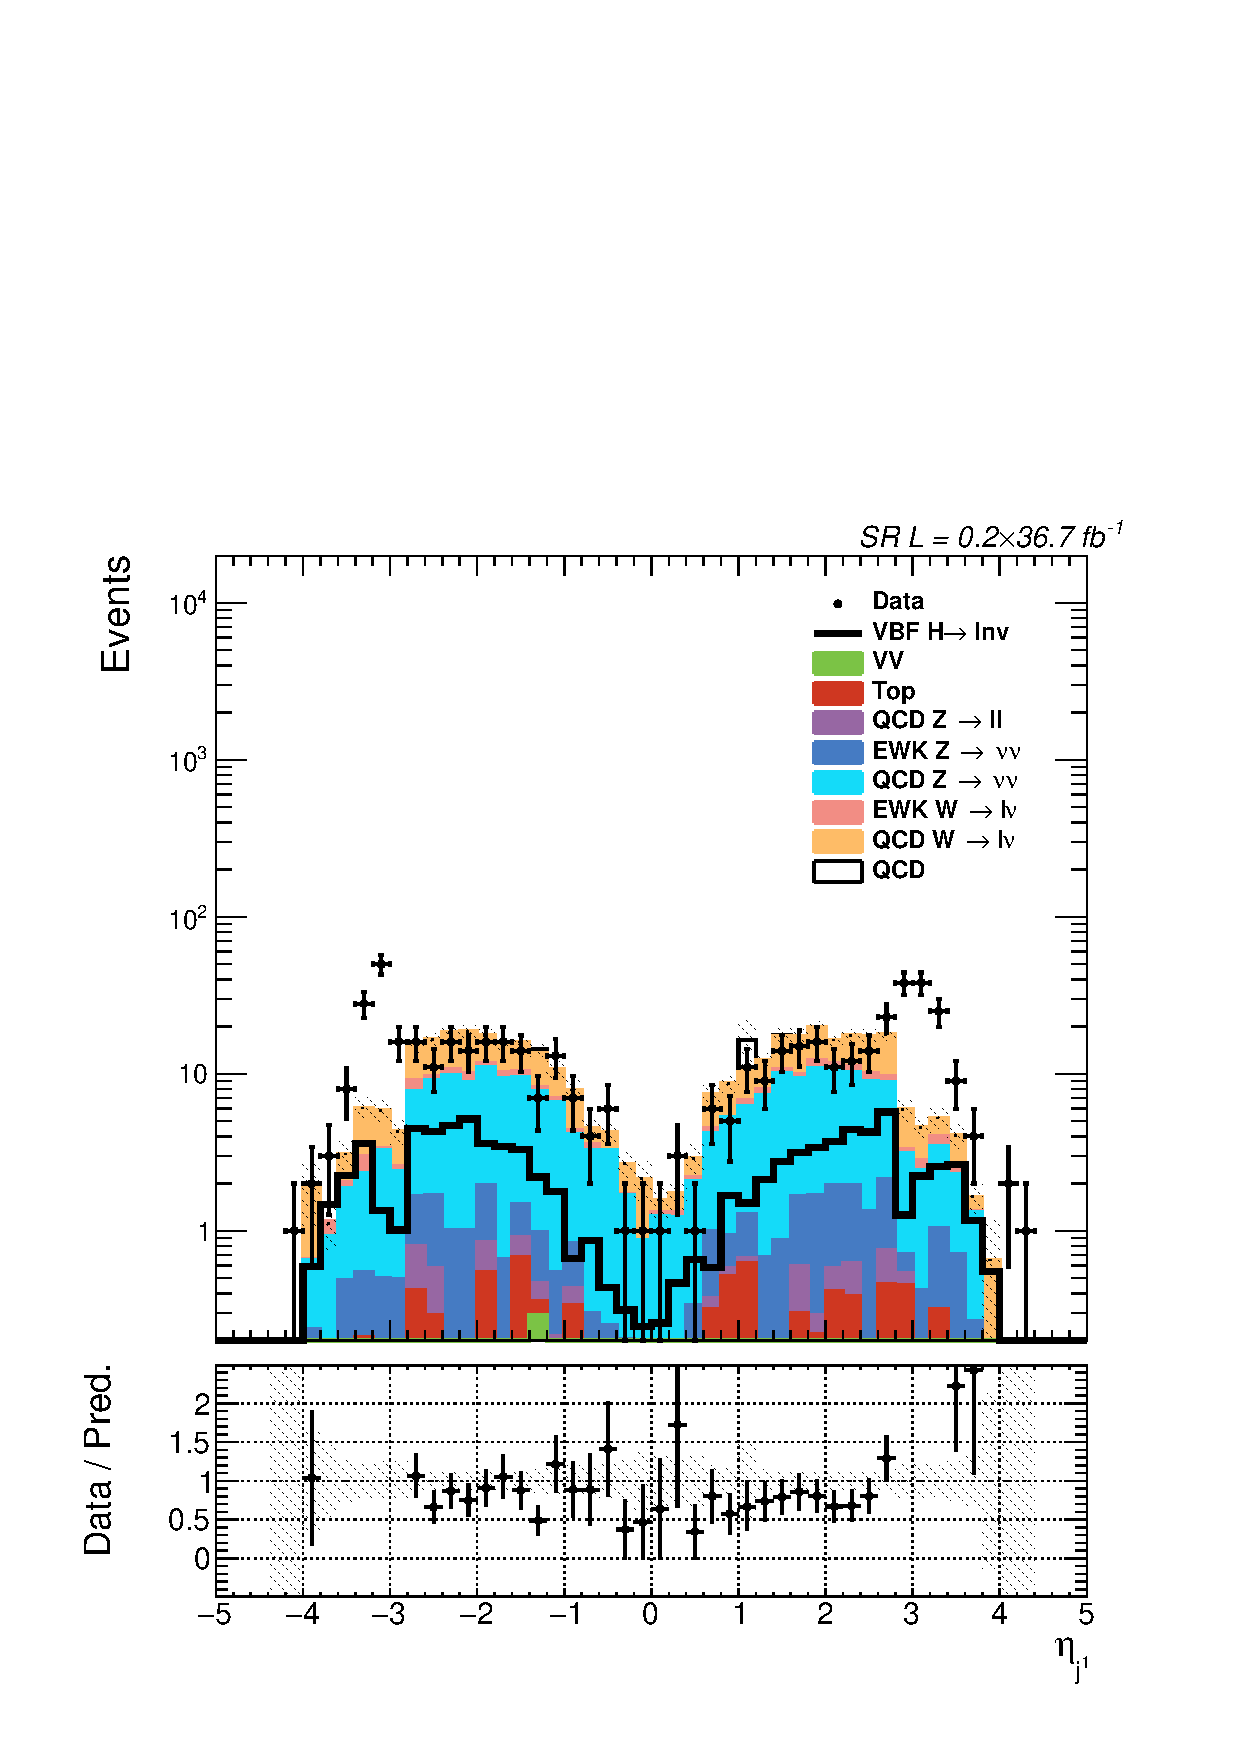
\includegraphics[width=0.49\textwidth]{Analysis_strategy/2017_postHornCut/VTRLeading_jet_eta_log.pdf}
    }
    \subfigure[$\eta_{j2}$ - VTR]{
    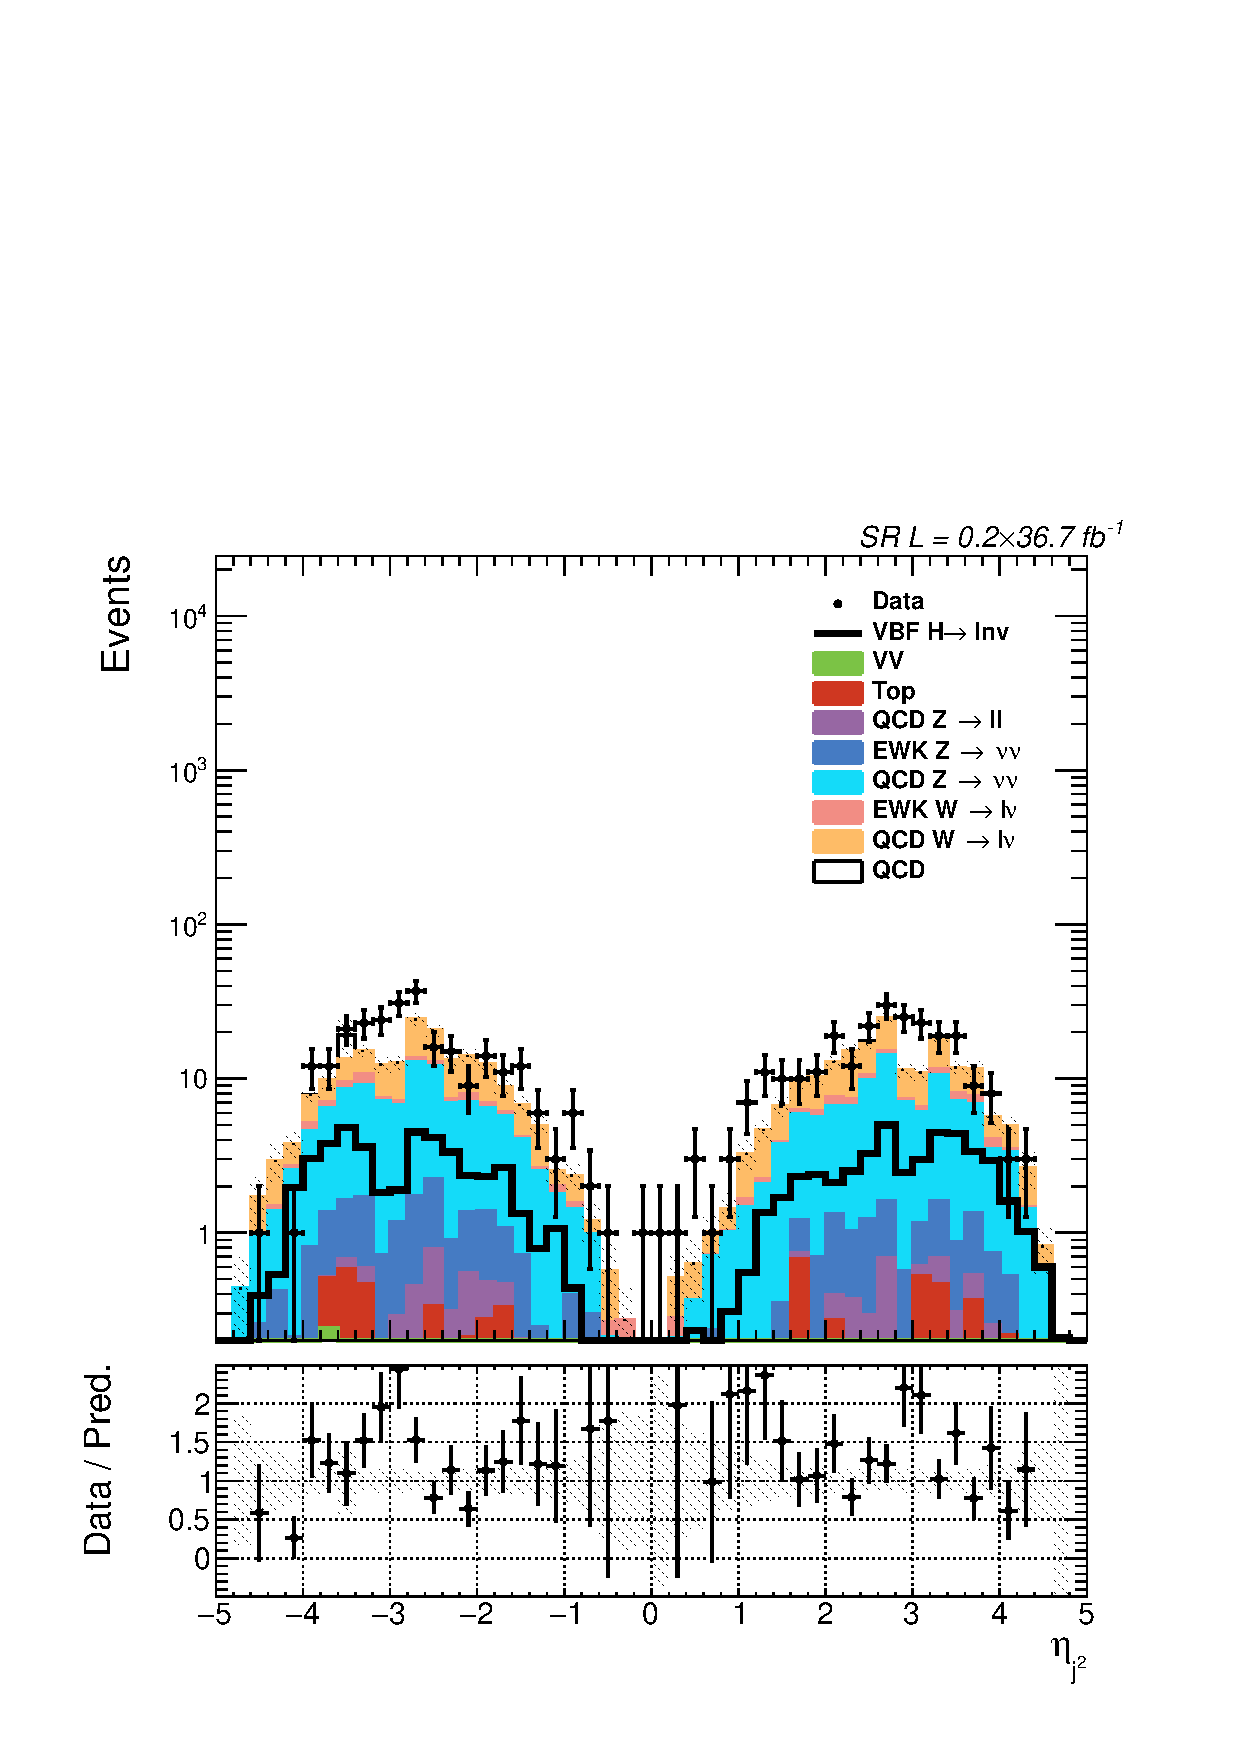
\includegraphics[width=0.49\textwidth]{Analysis_strategy/2017_postHornCut/VTRSubleading_jet_eta_log.pdf}
    }
  \caption{Distributions of $\eta_{j1}$ (left) and $\eta_{j2}$ (right) variables in the signal region after the unbinding of 1/5th of the 2017 data and the mitigation of the jet "horns" effect. Both MTR (top) and VTR (bottom) categories are presented.}
  \label{fig:jet_eta_postHornCut}
\end{figure}


\begin{figure}[htbp]
  \centering
    \subfigure[1-$E_{T,miss}^{~track}$/$E_{T, miss}$ - MTR]{
    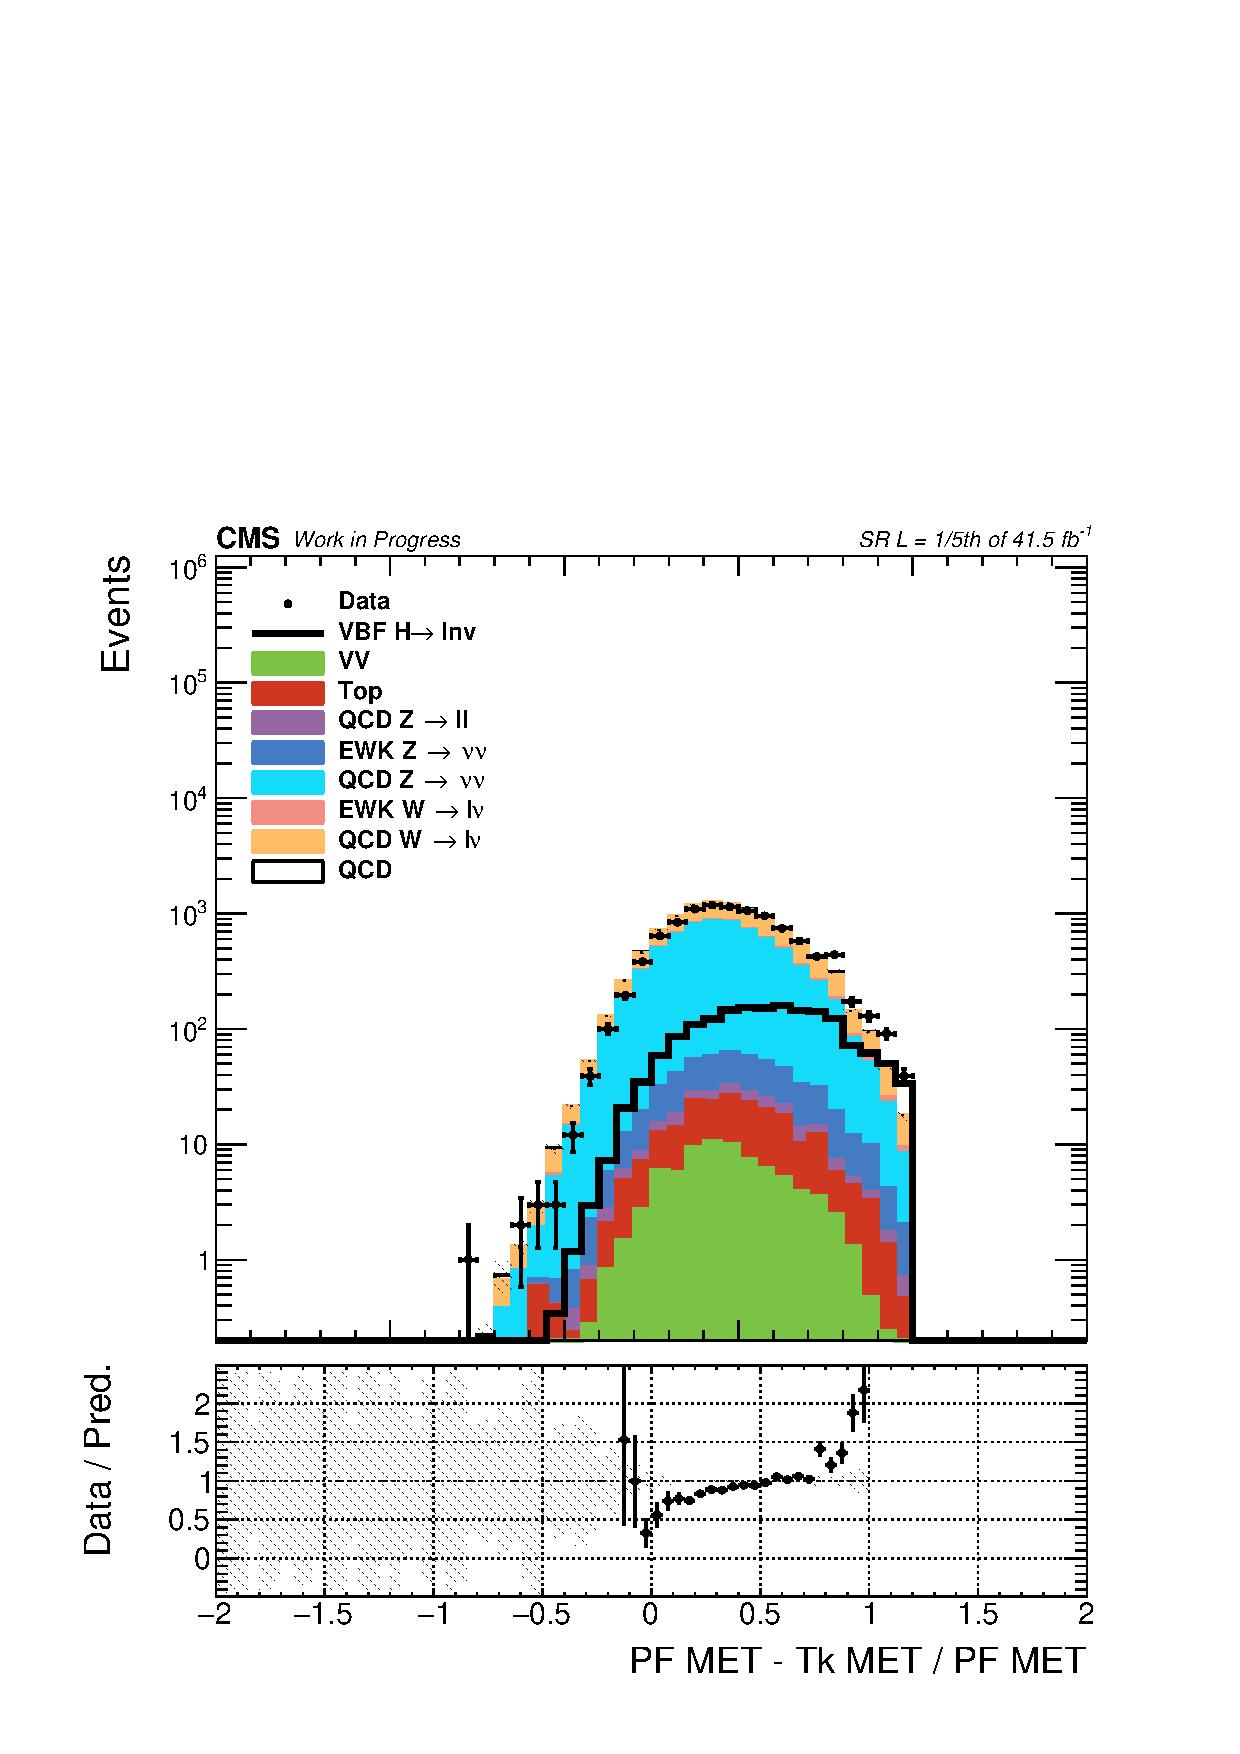
\includegraphics[width=0.49\textwidth]{Analysis_strategy/2017_postHornCut/TkMET_reldiff_MET_log.pdf}
    }
    \subfigure[1-$E_{T,miss}^{~track}$/$E_{T, miss}$ - VTR]{
    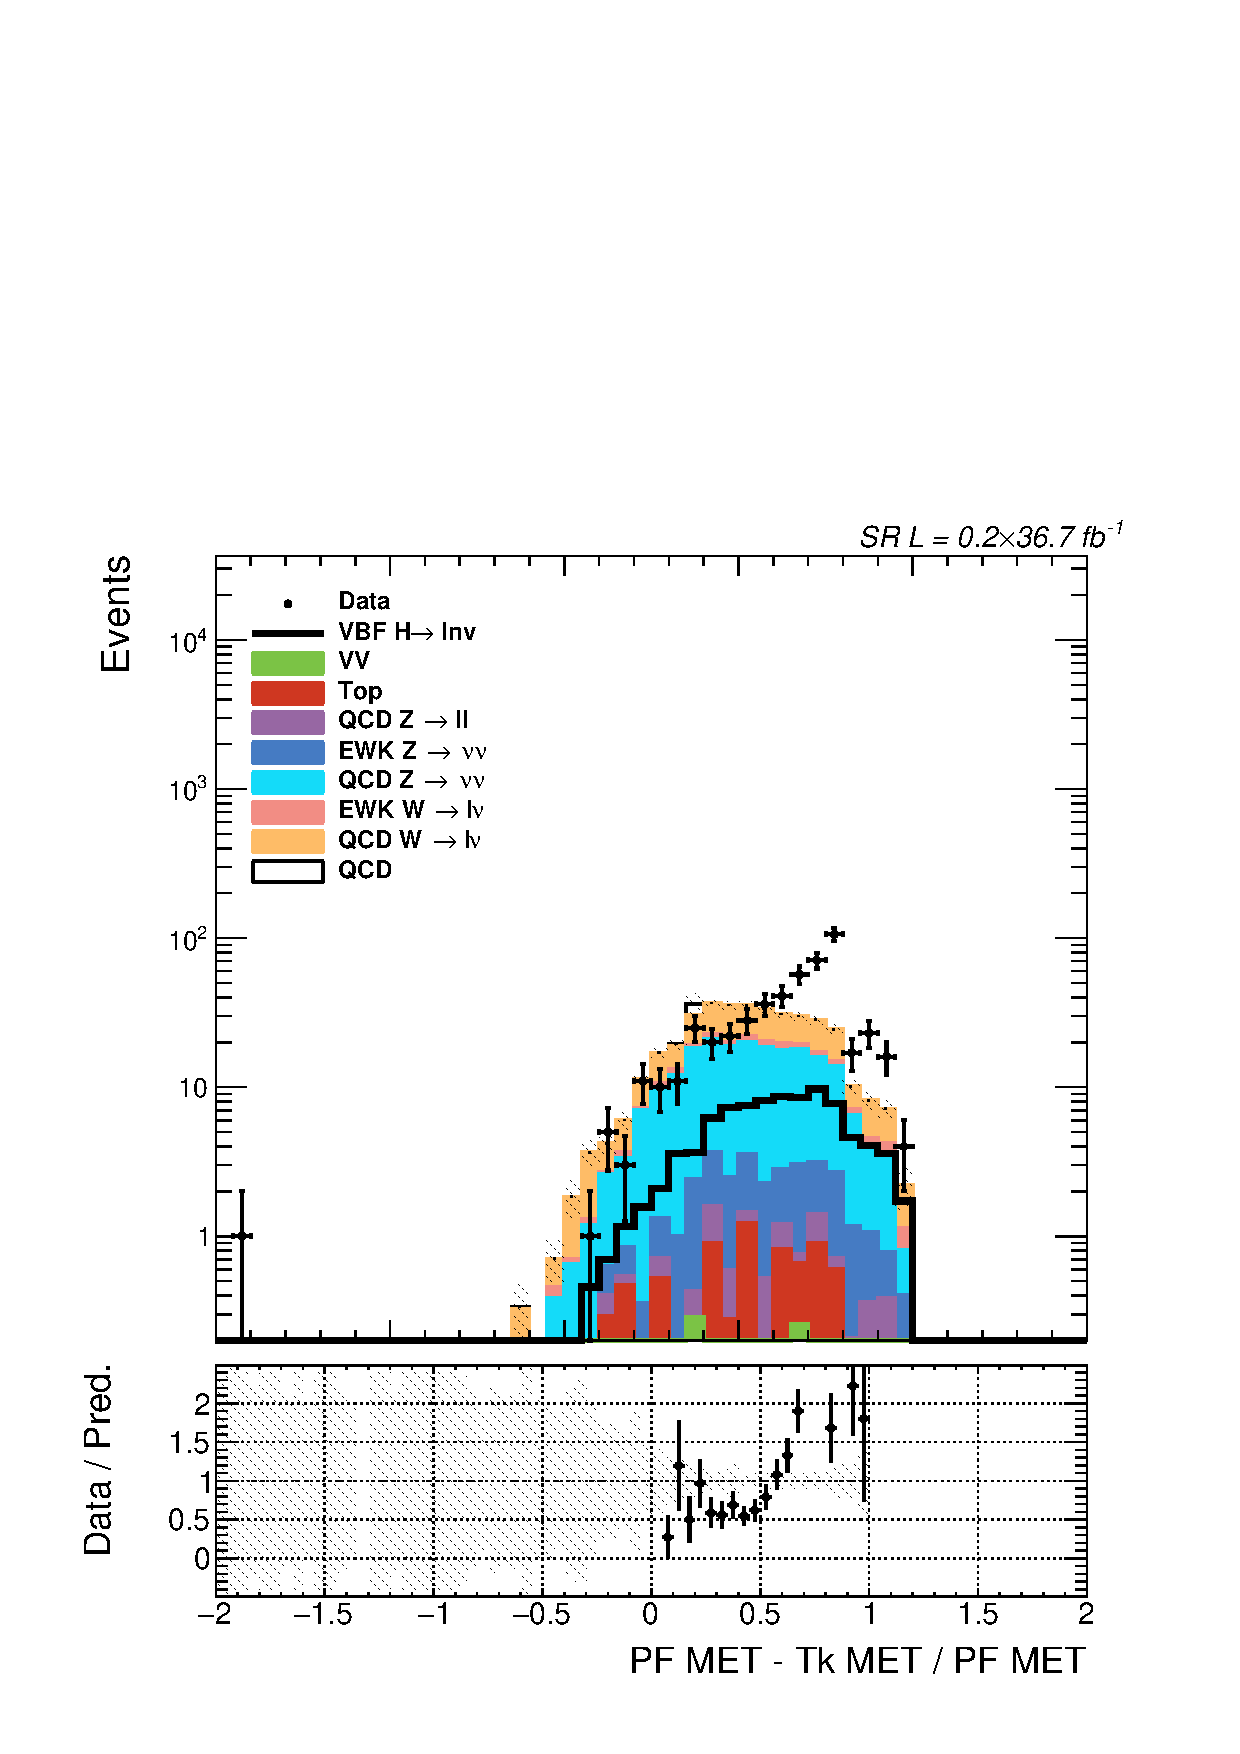
\includegraphics[width=0.49\textwidth]{Analysis_strategy/2017_postHornCut/VTRTkMET_reldiff_MET_log.pdf}
    }
  \caption{Distributions of the 1-$E_{T,miss}^{~track}$/$E_{T, miss}$ variable in the signal region after the unbinding of 1/5th of the 2017 data and the mitigation of the jet "horns" effect. Both MTR (left) and VTR categories are represented.}
  \label{fig:2017_postHornCut_met_vs_tkmet}
\end{figure}

\subsection{Missing HE sectors}
\hspace{10pt} The incident leaving a large amount of data collected during 2018 without any information about HCAL sectors 15/16 was the main motivation driving these, partial unblinding, studies. Being interested in forward jets, this analysis was especially affected in two regions, the signal and the electron regions. The latter is going to be discussed in more detail in Section~\ref{sec:single_electron}. The reason why this is problematic is connected with the position of the subdetectors, The affected region, observed from the point of view of the jet $\eta$ is -2.5$<\eta<$-1.4, thus marking an area which has a higher probability of jets faking the electrons.

\hspace{10pt} Another potential problem can happen if the PF candidate in the problematic range fails to be associates with the ECAL cluster of tracks. Following that there is no HCAL information in this HE-missing (HEM) region, this can be seen in the appearance of fake $E_{T,miss}$ populating the $\phi$ area covered by the HEM region. In order to test the SR for problems associated to the HEM region, the distribution of $\phi$ variable associated to the $\vec{p}_{T, miss}$ has been looked at. Figure~\ref{fig:hem_met} shows the data to simulation comparison of this variable for both the MTR and VTR categories, indicating a significant discrepancy in the -1.8$<\phi<$-0.6 region. Figures~\ref{fig:jet_phi_preHEM} shows the appearance of a similar discrepancy for the leading/subleading jet $\phi$ in the opposite side in $\phi$, as influenced by the signal selection. 


\begin{figure}[htbp]
  \centering
    \subfigure[$E_{T,miss}$ - MTR]{
    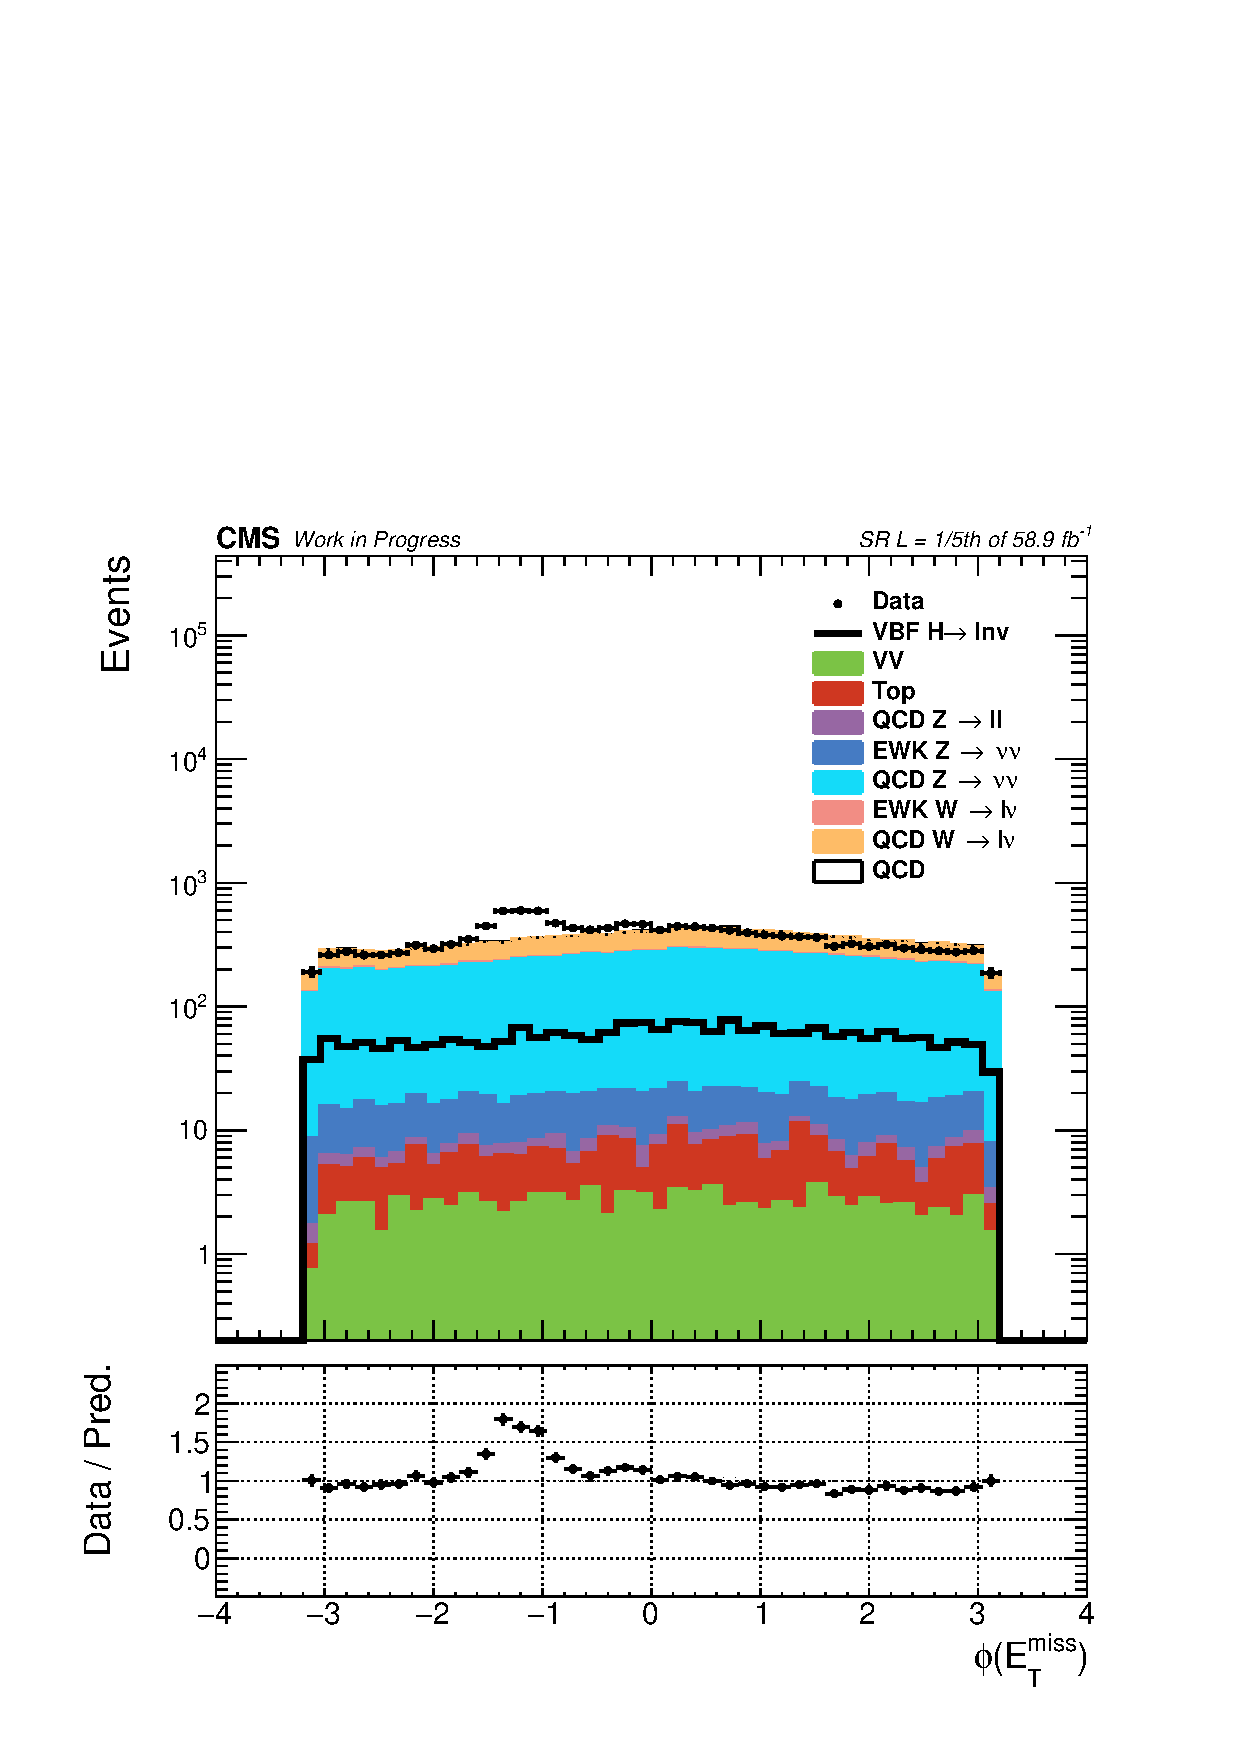
\includegraphics[width=0.49\textwidth]{Analysis_strategy/preHEMveto/MET_phi_log.pdf}
    }
    \subfigure[$E_{T,miss}$ - VTR]{
    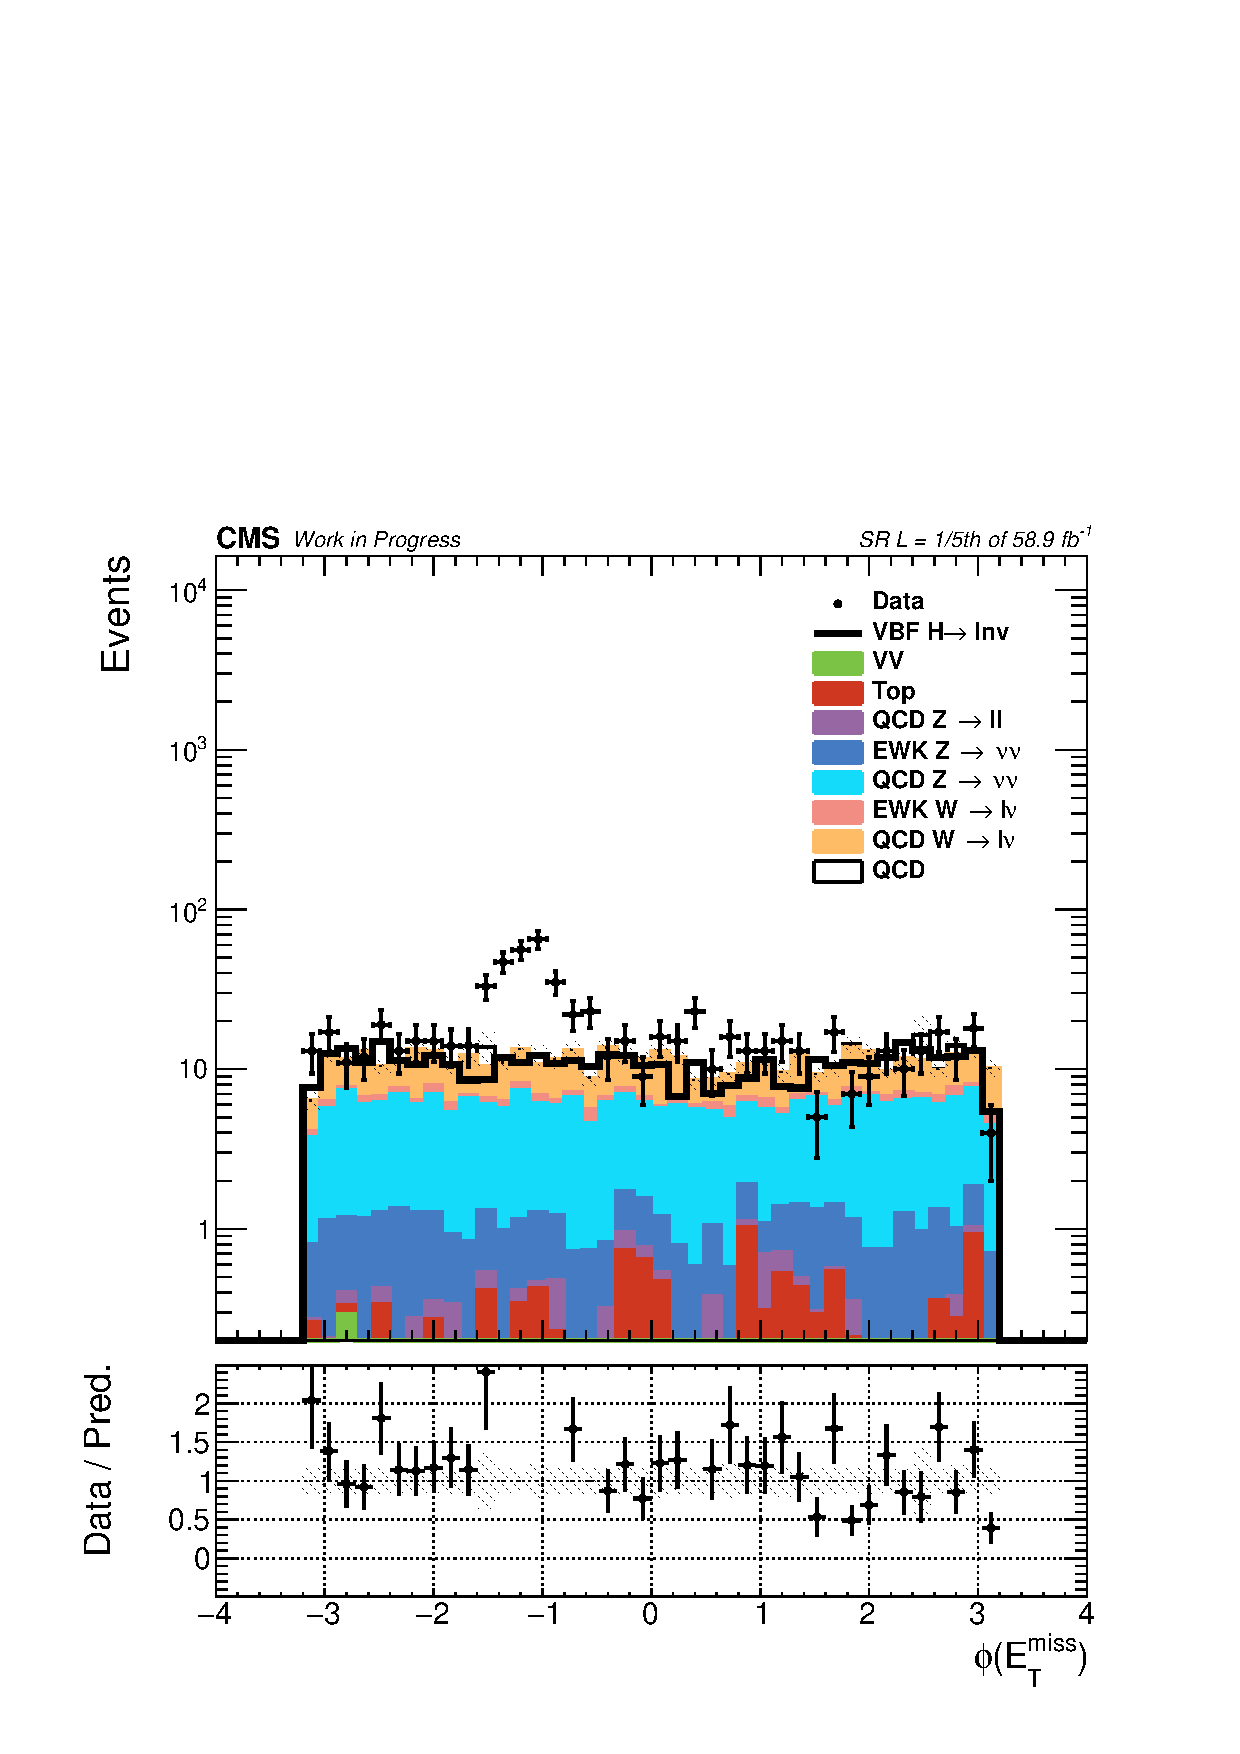
\includegraphics[width=0.49\textwidth]{Analysis_strategy/preHEMveto/VTRMET_phi_log.pdf}
    }
  \caption{Distributions of the $E_{T,miss}$ variable for the signal region presenting effects of the HEM problem for MTR (left) and VTR (right) categories.  }
  \label{fig:hem_met}
\end{figure}



\hspace{10pt} Upon performing a selection of studies with different jet quality requirements~\cite{note:AN_19_257}, the simplest solution was chosen for the end result. The whole $\phi$ region of the $\vec{p}_{T, miss}$ affected by the HEM problem was to be rejected from the selection requirements for the SR. Figure~\ref{fig:jet_phi_postHEM} shows distributions of leading and subleading jet $\phi$ after the application of the aforementioned veto. This has helped to return the overall data to simulaton agreement to the expected ranges, but it also brought in a loss sensitivity with respect to the B(H$\rightarrow$inv.) of $\sim$11~\%. The resulting veto has been added to the selection requirements for the 2018 era for both categories.

\begin{figure}[htbp]
  \centering
    \subfigure[$\phi_{j1}$ - MTR]{
    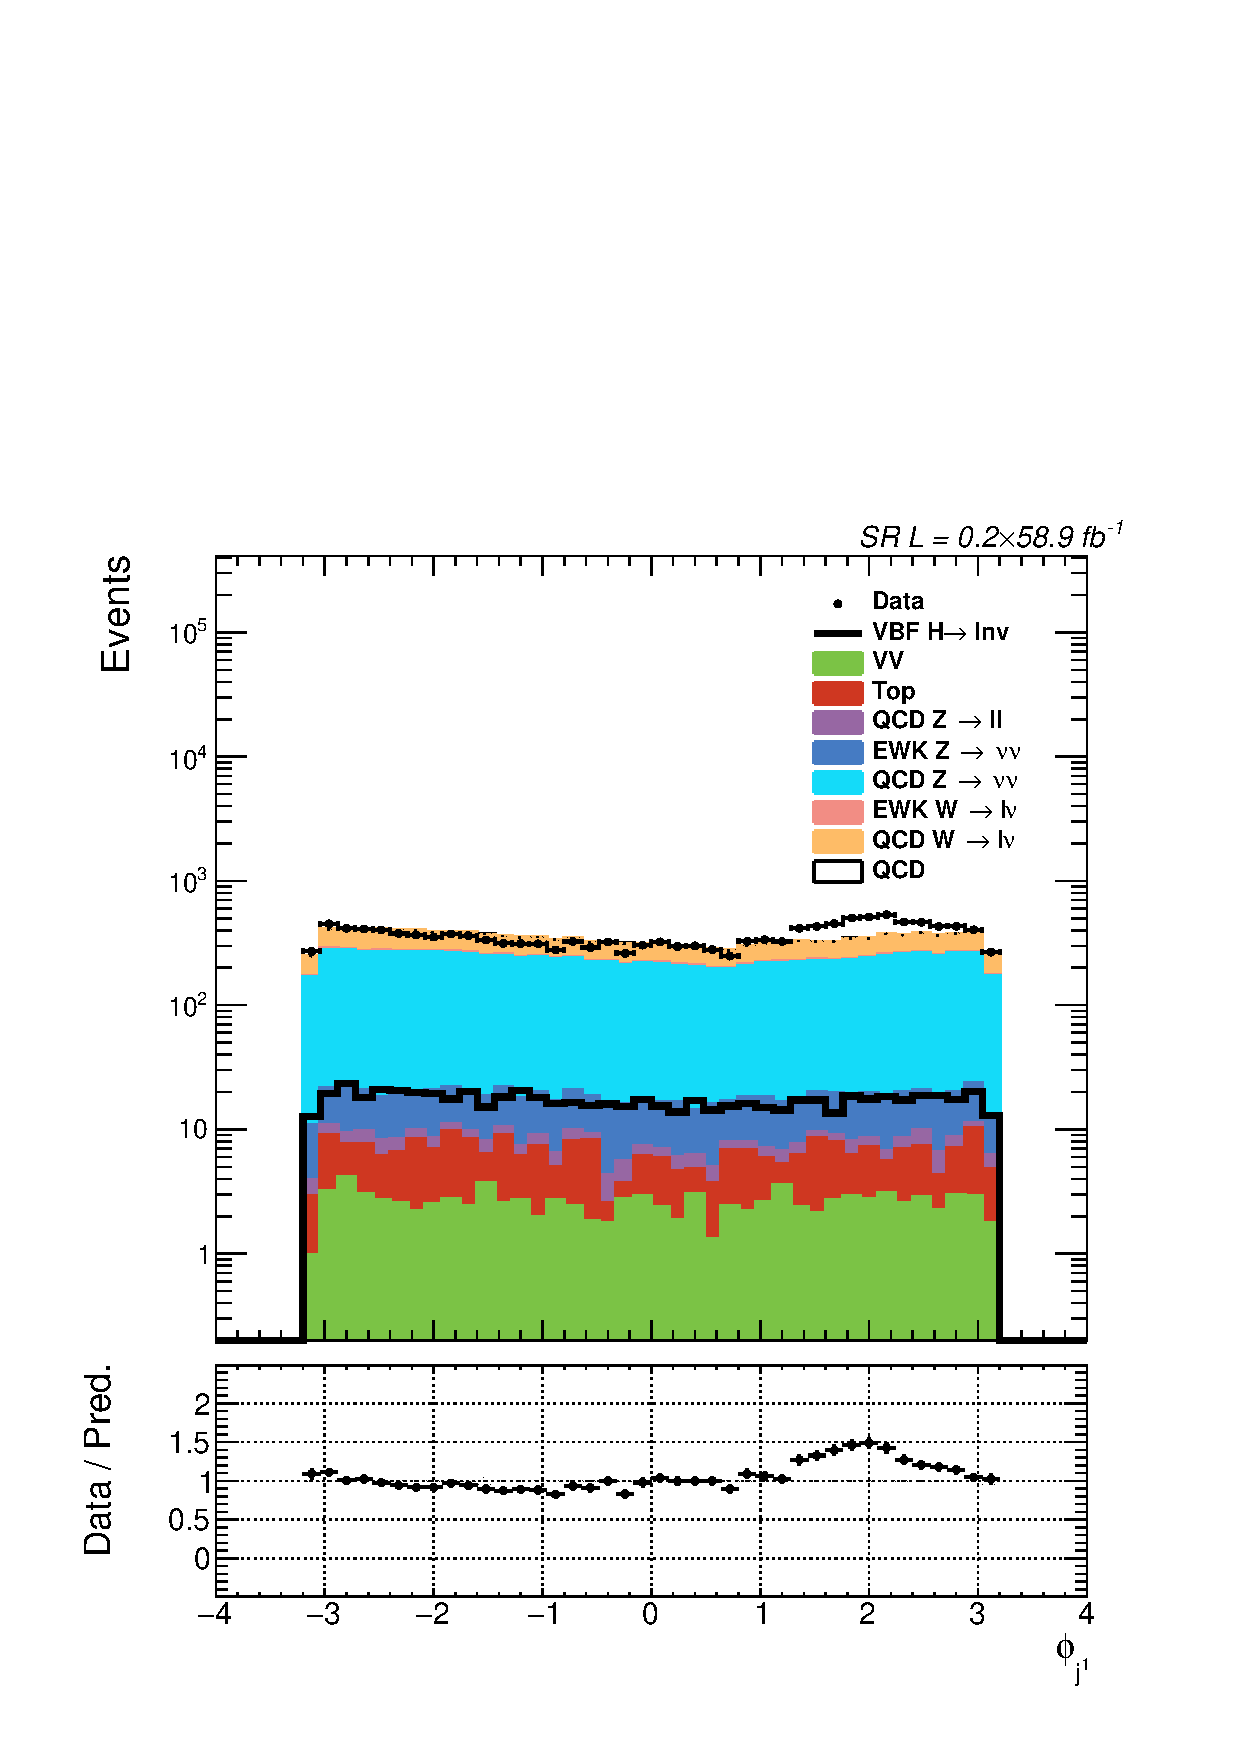
\includegraphics[width=0.49\textwidth]{Analysis_strategy/preHEMveto/Leading_jet_phi_log.pdf}
    }
    \subfigure[$\phi_{j2}$ - MTR]{
    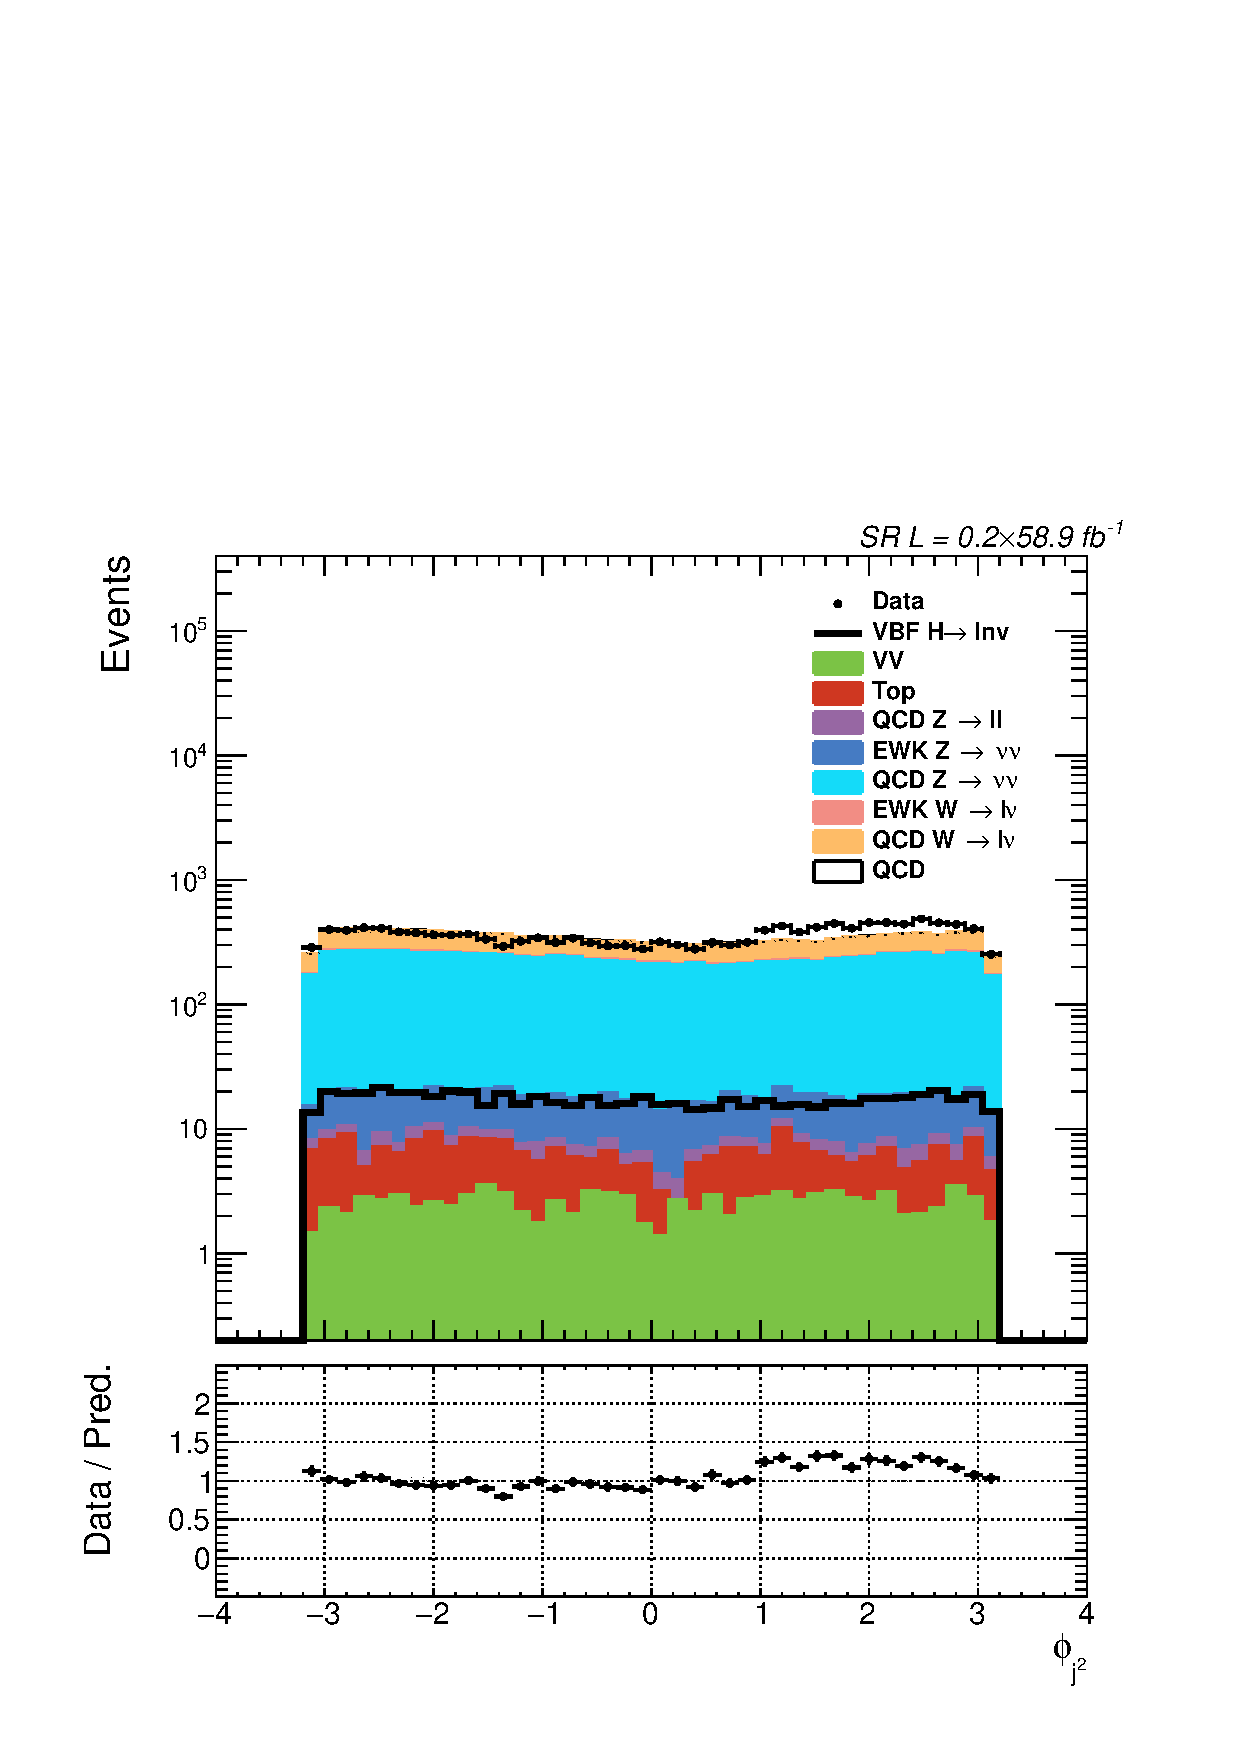
\includegraphics[width=0.49\textwidth]{Analysis_strategy/preHEMveto/Subleading_jet_phi_log.pdf}
    }\\
    \subfigure[$\phi_{j1}$ - VTR]{
    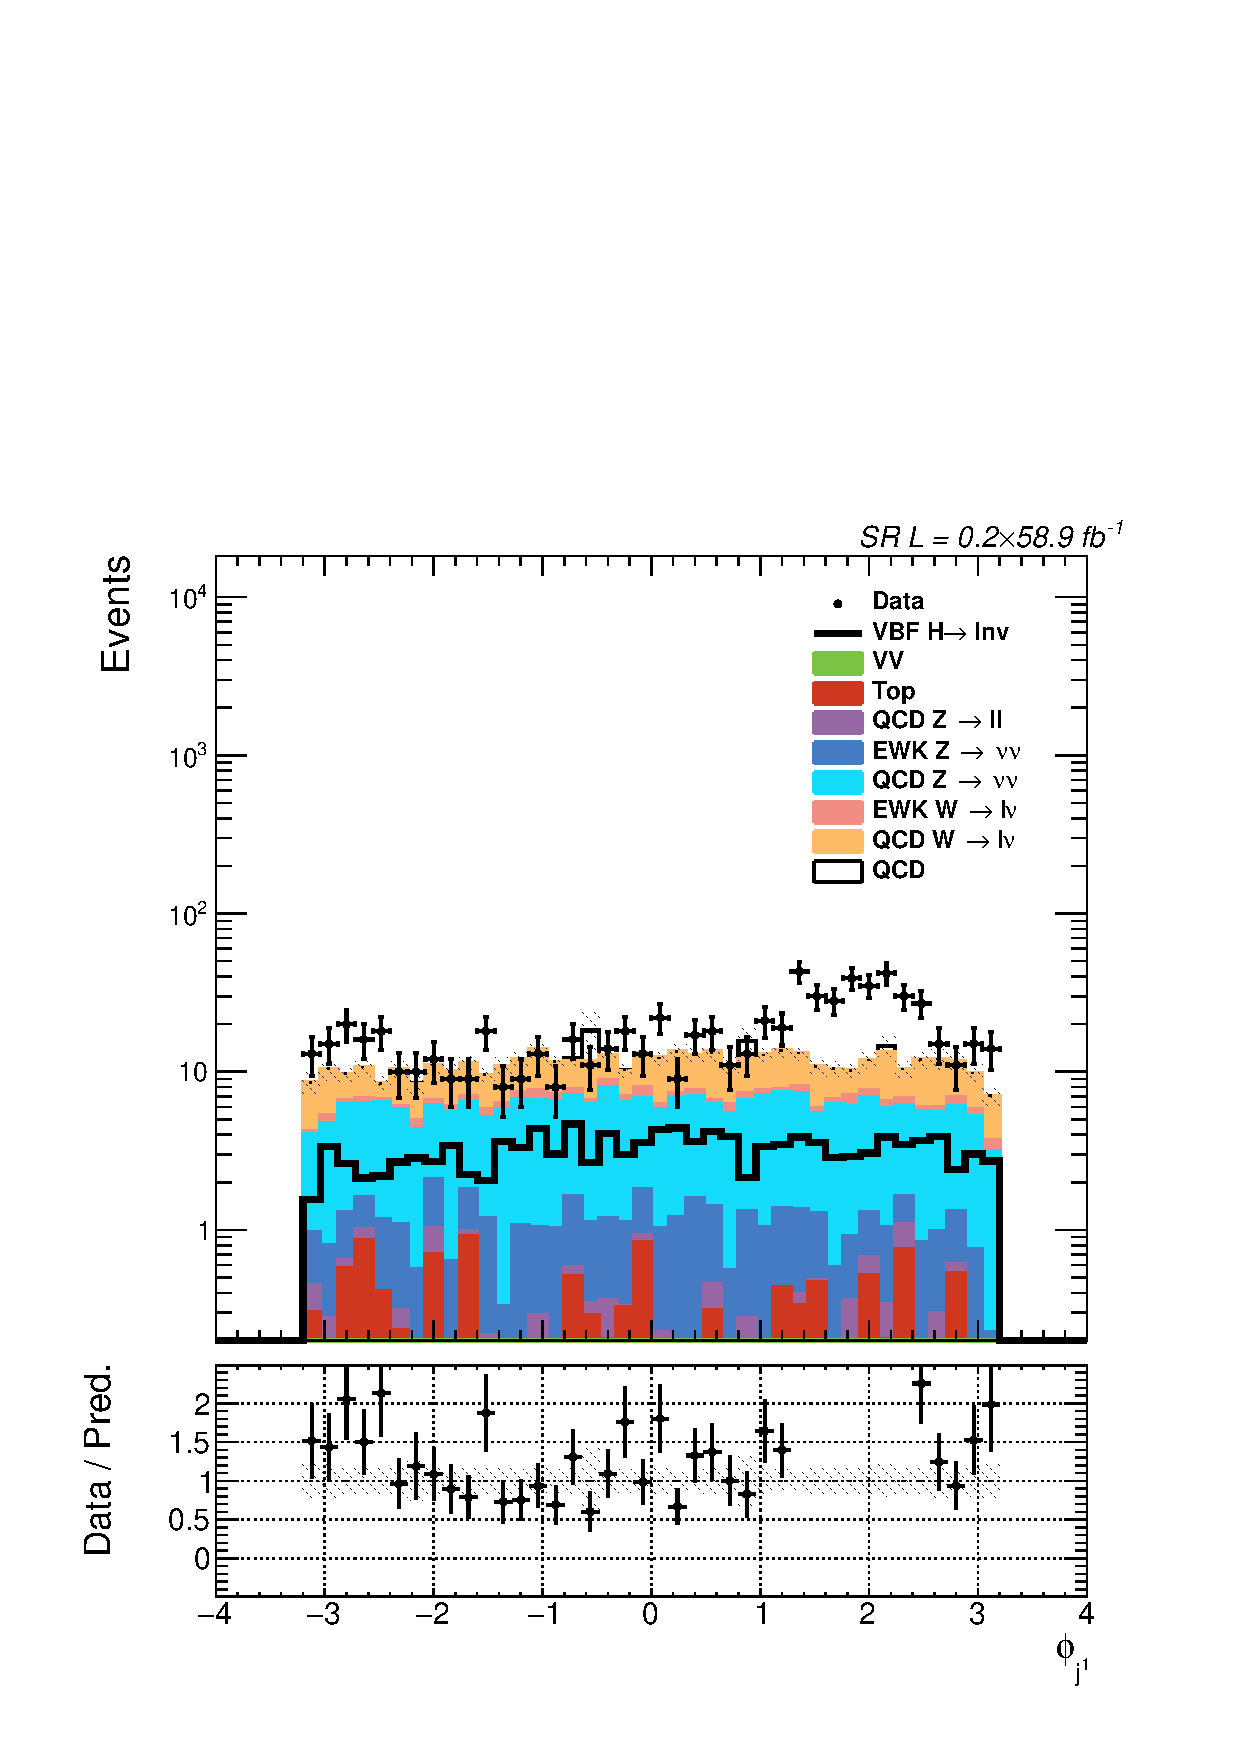
\includegraphics[width=0.49\textwidth]{Analysis_strategy/preHEMveto/VTRLeading_jet_phi_log.pdf}
    }
    \subfigure[$\phi_{j2}$ - VTR]{
    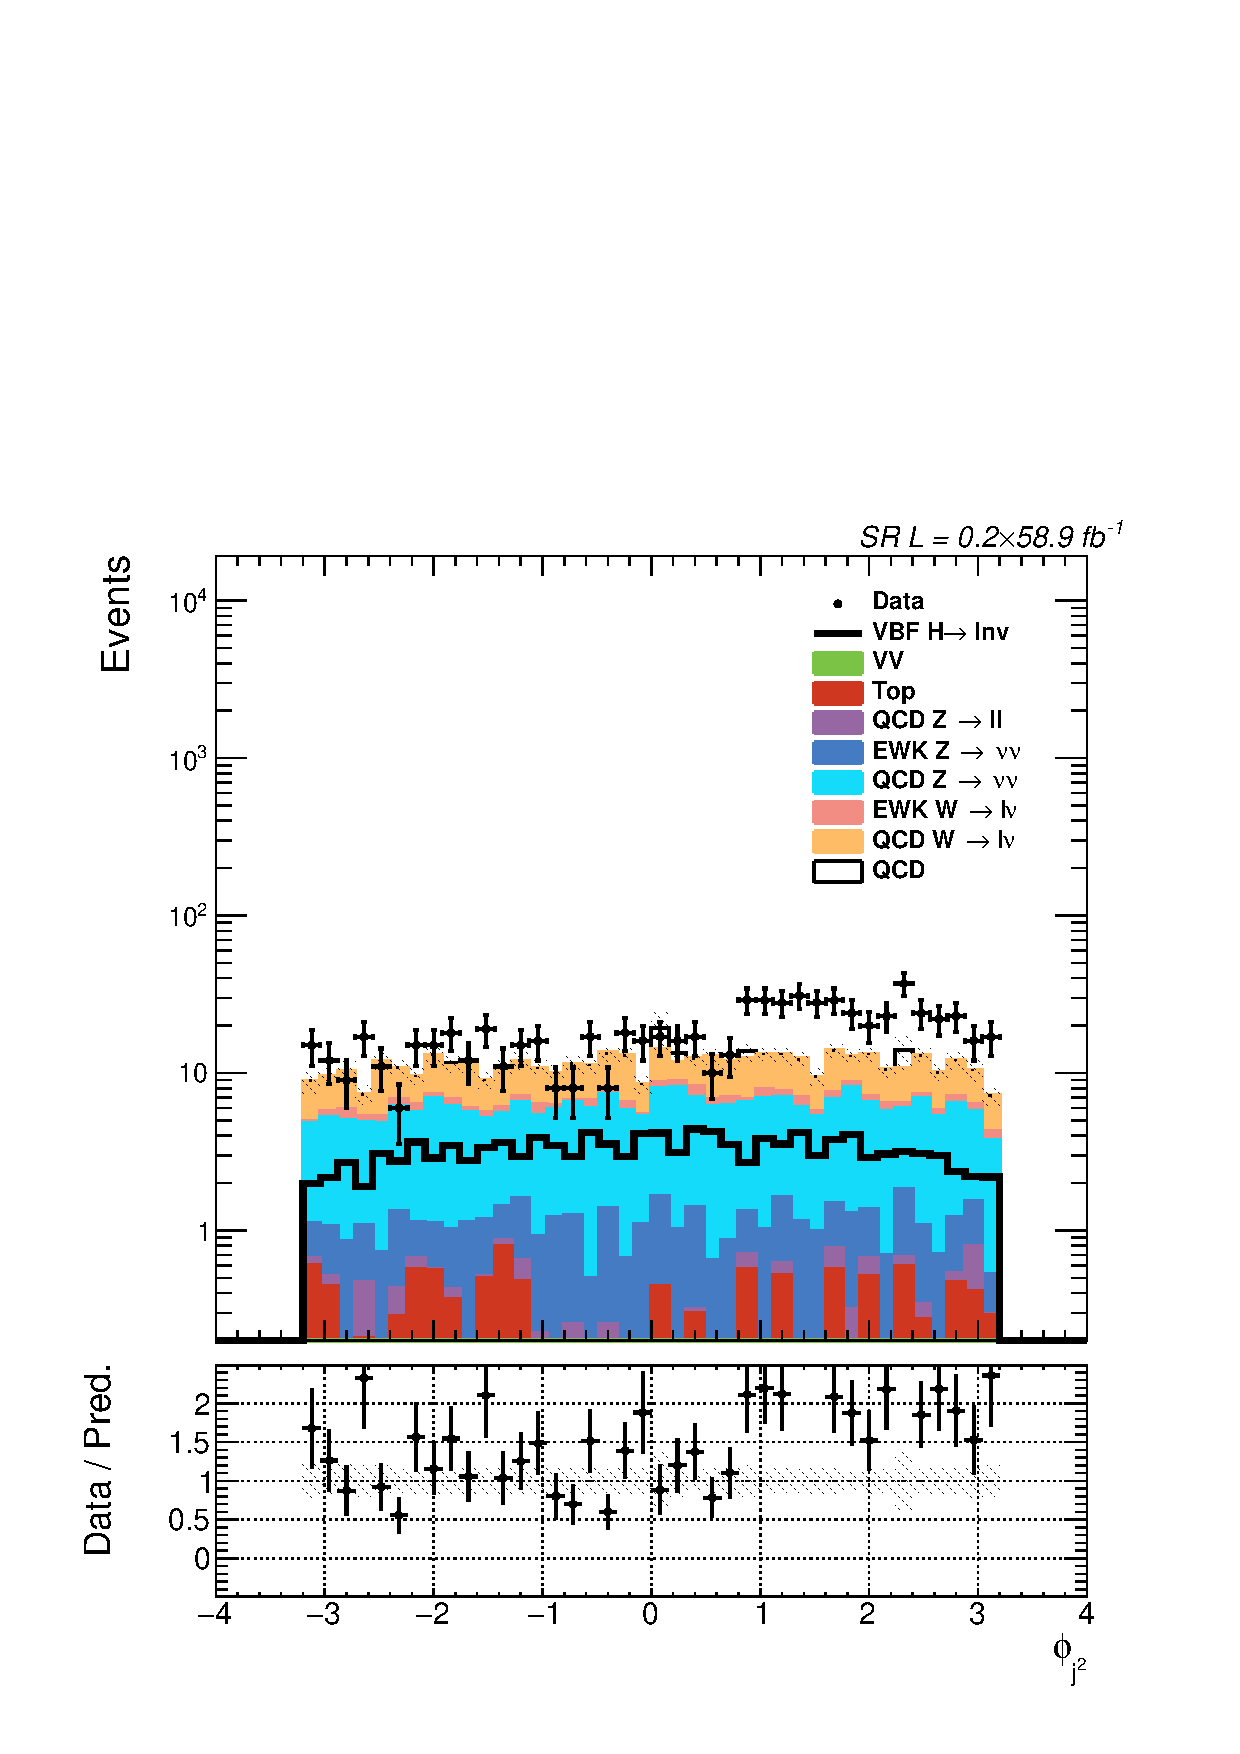
\includegraphics[width=0.49\textwidth]{Analysis_strategy/preHEMveto/VTRSubleading_jet_phi_log.pdf}
    }
  \caption{Distributions of $\phi_{j1}$ (left) and $\phi_{j2}$ (right) variables in the signal region, after the unbinding of 1/5th of the 2018 data, showing the effect of the HEM problem. Both MTR (top) and VTR (bottom) categories are presented.}
  \label{fig:jet_phi_preHEM}
\end{figure}


\begin{figure}[htbp]
  \centering
    \subfigure[$\phi_{j1}$ - MTR]{
    \includegraphics[width=0.49\textwidth]{Analysis_strategy/postHEMveto/Leading_jet_phi_log.pdf}
    }
    \subfigure[$\phi_{j2}$ - MTR]{
    \includegraphics[width=0.49\textwidth]{Analysis_strategy/postHEMveto/Subleading_jet_phi_log.pdf}
    }\\
    \subfigure[$\phi_{j1}$ - VTR]{
    \includegraphics[width=0.49\textwidth]{Analysis_strategy/postHEMveto/VTRLeading_jet_phi_log.pdf}
    }
    \subfigure[$\phi_{j2}$ - VTR]{
    \includegraphics[width=0.49\textwidth]{Analysis_strategy/postHEMveto/VTRSubleading_jet_phi_log.pdf}
    }
  \caption{Distributions of $\phi_{j1}$ (left) and $\phi_{j2}$ (right) variables in the signal region, after the unbinding of 1/5th of the 2018 data and following the mitigation of the HEM problem. Both MTR (top) and VTR (bottom) categories are presented.}
  \label{fig:jet_phi_postHEM}
\end{figure}